\usepackage[utf8]{inputenc}

\usepackage[printonlyused,withpage]{acronym}
\usepackage{amsmath,amssymb,amsthm}
\usepackage{algorithm}
\usepackage{algpseudocode}
\usepackage[USenglish]{babel}
\usepackage[
    style=ieee,
    backend=biber,
    url=false,
    doi=true,
    eprint=false,
    sorting=none
]{biblatex}
\usepackage{booktabs}
\usepackage{color}
\usepackage{epigraph}
\usepackage{enumitem}
\usepackage{float}
\usepackage{graphicx}
\usepackage[hidelinks]{hyperref}
\usepackage{listings}
\usepackage{listings-rust/listings-rust}
\usepackage{makecell}
\usepackage{mathtools}
\usepackage{mathrsfs}
% No indent after paragraphs
\usepackage{parskip}
\usepackage{siunitx}
\usepackage{tabularx}
\usepackage{tikz}
\usepackage{onimage}

% /--- See https://www.tug.org/FontCatalogue/ ------------------------------------------------------
% \-------------------------------------------------------------------------------------------------

% /--- Everything about fancyhdr -------------------------------------------------------------------
\usepackage{fancyhdr}
% \fancyhead{} % clear all header fields
\fancyfoot{} % clear all footer fields
\fancyhead[L]{\rightmark}
\fancyhead[R]{Jonas Pleyer}
\fancyfoot[RO,LE]{\thepage}

\fancypagestyle{plain}{% % <-- this is new
    \fancyfoot{} % clear all footer fields
    \fancyhead{} % clear all header fields
    \fancyfoot[RO,LE]{\thepage}
\renewcommand{\headrulewidth}{0pt}}% remove rule

\setlength{\headheight}{13.6pt}
% \-------------------------------------------------------------------------------------------------

% Configure lstlistings
\definecolor{beige}{RGB}{255, 245, 240}
\lstset{
    backgroundcolor=\color{beige},
    frame=single,
    keepspaces=true,
    captionpos=b,
    breaklines=true,
}

\addbibresource{references.bib}

\DeclareSIUnit\pixel{pixel}

\newcommand{\subtitle}{On Theory, Implementation and Application}

\makeatletter
\title{Agent-Based Models in Cellular Systems}\let\Title\@title
\author{Jonas Pleyer}\let\Author\@author
\date{01.04.2026}\let\Date\@date
\makeatother

\numberwithin{equation}{chapter}

\setlist{noitemsep}

\usepackage{setspace}
\onehalfspacing

% Define epigraph (quotations at beginning of every section)
\setlength\epigraphwidth{0.7\textwidth}
% \renewcommand{\epigraphflush}{flush}
\renewcommand{\beforeepigraphskip}{0.0cm}
\renewcommand{\afterepigraphskip}{2.0cm}

% Define style for chapter heading
\usepackage{titlesec}
\titleformat
{\chapter}% command
[display]% shape
{\bfseries\huge}% format
{\Large Chapter \thechapter}% label
{0.5ex}% sep
{}% before code
[\vspace{-0.5ex}\rule{\textwidth}{0.3pt}] % after-code

\titlespacing{\chapter}{0cm}{0cm}{0.5cm}

\newcommand{\R}{\mathbb{R}}
\newcommand{\CS}{\mathscr{C}}
\newcommand{\EV}{\mathscr{E}}

% Define definition, example, lemma, proof and theorem.
\newtheorem{definition}{Definition}[section]
\newtheorem{example}[definition]{Example}
\newtheorem{lemma}[definition]{Lemma}
\newtheorem{corollary}[definition]{Corollary}
\newtheorem{theorem}[definition]{Theorem}

% \renewcommand*{\chapterheadstartvskip}{\vspace*{0cm}}
% \renewcommand*{\chapterheadendvskip}{\vspace{0cm}}

\raggedbottom

% Add todonotes package
\usepackage{todonotes}
\setuptodonotes{color=blue!30}

\includeonly{%
    01-introduction,%
    02-elongated-bacteria,%
    03-cellular-raza,%
    04-abm-theory,%
    05-bacterial-rods,%
    06-further-applications,%
    07-discussion,%
    08-conclusion,%
    20-supplement,%
    declaration,%
}


\begin{document}
% TITLEPAGE

\pagestyle{fancy}
\renewcommand{\sectionmark}[1]{\markright{\thesection~ ~#1}}
% \renewcommand{\chaptermark}[1]{\markboth{\chaptername~\thechapter~-~ #1}{}}

\pdfbookmark[1]{Titlepage}{titlepage}
\begin{titlepage}
    % Turns off page numbering
    \pagenumbering{Alph}
    \thispagestyle{empty}
    \begin{center}

        \Large\textbf{ALBERT-LUDWIGS-UNIVERSITÄT\\ FREIBURG IM BREISGAU\\}
        \vspace{0.5cm}
        \Large\textbf{Institute of Physics}

        \rule{\textwidth}{1pt}
        \vspace{1.5cm}

        \huge\textbf{\Title}
        \Large\textbf{\subtitle}

        \vspace{1.5cm}

        \includegraphics[width=0.6\textwidth]{logos/uni-fr-sigil-black.png}

        %\vspace{18cm}
        \vfill

        \Large{Dissertation}\\
        \normalsize
        zur Erlangung des Doktorgrades\\
        % Doctoral Thesis in Physics\\
        \vspace{0.5cm}
        submitted \Date\hspace{0pt} by\\
        \vspace{0.5cm}
        \Large\textbf{Jonas Pleyer}\\
        \normalsize
        \vspace{0.5cm}
        % born in Heidelberg (Germany)\\
        \large Supervisor: Dr. Christian Fleck\\
        \large Supervisor: Prof. Dr. Jens Timmer\\
        \normalsize

        \newpage\null\thispagestyle{empty}
        % Here but anything like ISBN or whatever credentials of the final binding might be
        % required.
        \newpage
        \thispagestyle{empty}
        \newpage
        I thank my wife Anja for her unweary support and love.

    \end{center}
\end{titlepage}
\thispagestyle{empty}


\newpage
\pagenumbering{Roman}
\pdfbookmark[0]{Contents}{contents}
\tableofcontents
\newpage

\pdfbookmark[1]{\listfigurename}{listoffigures}
\listoffigures

\pdfbookmark[1]{\listtablename}{listoftables}
\listoftables

\pdfbookmark[1]{Listings}{listoflistings}
\lstlistoflistings

\chapter*{Acronyms}
\pdfbookmark[1]{Acronyms}{listofacronyms}
\begin{acronym}
    % Modeling related acronyms
    \acro{abm}[ABM]{Agent-Based Model}
    \acro{cabm}[CABM]{Cellular Agent-Based Model}
    \acro{cabmf}[CABMF]{cell-agent-based model framework}
    \acro{ode}[ODE]{Ordinary Differential Equation}
    \acro{sde}[SDE]{Stochastic Differential Equation}
    \acro{pde}[PDE]{Partial Differential Equation}
    \acro{ca}[CA]{Cellular Automaton}
    \acroplural{ca}[CA]{Cellular Automata}
    \acro{cpm}[CPM]{Cellular Pottes Model}
    \acro{ib}[IB]{Individual-Based}
    \acro{dfba}[DFBA]{Diffusion Flux Balance Analysis}

    % Biology-specific Modeling
    \acro{ir}[IR]{Intracellular Reaction}
    \acro{er}[ER]{extracellular reaction}
    \acro{rd}[RD]{reaction-diffusion}
    \acro{ggh}[GGH]{Glazier-Graner-Hogeweg}
    \acro{grn}[GRN]{Gene Regulatory Network}
    \acro{jkr}[JKR]{Johnson-Kendall-Roberts}
    % \acro{pbpk}[PBPK]{Physiologically Based Pharmacokinetic}
    \acro{sbml}[SBML]{Systems Biology Markup Language}
    \acro{tp}[TP]{Turing-pattern}

    % Technical words
    \acro{msd}[MSD]{Mean Squared Displacement}
    \acro{ls}[LS]{Least Squares}
    \acro{gpu}[GPU]{Graphics Processing Unit}
    \acro{gui}[GUI]{Graphical User Interface}
    \acro{os}[OS]{open source}
    \acro{lcd}[LCD]{Liquid Crystal Display}

    % Bacterial Species
    \acro{ecoli}[\textit{E.coli}]{\textit{Escherichia coli}}
    \acro{bsubtilis}[\textit{B.subtilis}]{\textit{Bacillus subtilis}}
    \acro{paeruginosa}[\textit{P.aeruginosa}]{\textit{Pseudomonas aeruginosa}}
    \acro{flavo}[\textit{F. johnsoniae}]{\textit{Flavobacterium johnsoniae}}
    \acro{serratia}[\textit{S. marcescens}]{\textit{Serratia marcescens}}
    % Other
    \acro{pg}[PG]{Peptidoglycan}
    \acro{a22}[A22]{S-(3,4-Dichlorobenzyl)isothiourea}
    \acro{mre}[\textit{Mre}]{Murein formation gene cluster E}
    \acro{tirf}[TIRF-M]{Total internal reflection Fluorescence Microscopy}
    \acro{ecm}[ECM]{Extracellular Matrix}
    \acro{qs}[QS]{Quorum Sensing}
    \acro{crispr}[CRISPR]{Clustered Regularly Interspaced Short Palindromic Repeats}
\end{acronym}


\chapter*{Preface \& Readers Guide}
\pdfbookmark[1]{Preface \& Readers Guide}{preface}
\begin{itemize}
    \item section 1: gives overview of everything and aims to build bridge between the topics
    \item section 2+3: conceptual, generalizable for many systems
    \item section 4+5: specific for elongated bacteria
    \item section 6: collection of many distinct applications
\end{itemize}

%###################################################################################################
\pagebreak

Kapitel 1 soll eine Einführung in ABMs geben. Dabei möchte ich vor Allem das Mini-Review
von uns verwenden und auf Gemeinsamkeiten, Unterschiede, und ein wenig Geschichte
eingehen. Hier möchte ich schon einige Ideen aufbringen, die später wieder aufgegriffen
werden. Diese habe ich erstmal als eigene Subsections gelistet.

%---------------------------------------------------------------------------------------------------
\section{Scales in Physics and Biology}
\begin{itemize}
    \item smallest proteins:
        \begin{itemize}
            \item \textit{spoVM} \cite{Levin1993} (sporulation in Bacillus subtilis)
            \item \textit{TAL peptide} (smallest naturally ocurring, discovered in
                Drosophila melanogaster in 2007) \cite{Galindo2007}
        \end{itemize}
    \item largest scales: population dynamics across continents (earth $\approx
        40'000\text{km}$ circumference)
\end{itemize}

%---------------------------------------------------------------------------------------------------
\section{Cellular Building Blocks}
\begin{itemize}
    \item complex organisms from collection of cells
    \item self-organization/pattern formation
    \item single-cell vs bulk
\end{itemize}

%---------------------------------------------------------------------------------------------------
\section{Comparison of Simulation Frameworks}
\begin{itemize}
    \item use mainly mini-review for this subsection \cite{Pleyer2023}
    \item many frameworks
    \item some similar approaches
    \item purpose-built solutions
    \item missing flexibility in model design or ability to apply to various systems
    \item large number of parameters which need to be supplied
\end{itemize}

%---------------------------------------------------------------------------------------------------
\section{Mathematical Treatment}
\begin{itemize}
    \item no "unfiying theory"
    \item with theoretical framework, we would be able to systematically discuss any of
        the following:
        \begin{itemize}
            \item coarse-graining
            \item uncertainty analysis
            \item dimensionality reduction
        \end{itemize}
\end{itemize}

%---------------------------------------------------------------------------------------------------
\section{Are we flexible yet?}
\begin{itemize}
    \item flexibility matters (why)
    \item show some examples: rust pear fungus (differing cell types interacting), budding yeast
        elongated bacteria (non-trivial geometry)
    \item we are not there yet
\end{itemize}

%---------------------------------------------------------------------------------------------------
\section{Are we calibrated yet?}
\begin{itemize}
    \item many \acp{abm} do not do proper parameter estimation
    \item what are we actually modeling here?
\end{itemize}

%---------------------------------------------------------------------------------------------------
\section{The mesoscopic approach}
\begin{itemize}
    \item physicists: natural tendency to go big (many particles, large scale), or go small
        (fine-grained look at things, sub-microscopig)
    \item no real natural tendency to go mesoscopic
    \item we operate on the scale of 1-100 cells making it sometimes feasible to employ statistics
        and sometimes feasible to account for natural cell-cell variability
    \item depends on specific cases all the time
\end{itemize}

\section{Introduction}
\label{sec:self-organization}
% Self-organization~\cite{camazineSelfOrganizationBiologicalSystems2020} is an energy
% consuming dynamic process in which the collective behavior of individual agents
% exhibits emergent phenomena by forming spontaneous order through interaction between
% the agents, i.e., exchange of information, without the need of an external controlling agent.
% The emerging patterns cannot directly be inferred by the properties of the individual
% agents and are typically robust with respect to perturbations.
% Self-organization needs to be distinguished from self-assembly, which \nt{results from
% minimization of the free energy of a thermodynamic}
% system~\cite{johnAlternativeMechanismsStructuring2005,dambricourtmalasseSelfOrganizationNewParadigm2022},
% e.g., the self-assembly of a lipid bilayer or the spontaneous folding of
% proteins~\cite{kuhlmanAdvancesProteinStructure2019,albertsLipidBilayer2002,wedlich-soldnerSelforganizationFundamentCell2018}.
% \nt{In contrast,} self-organization happens in non-equilibrium conditions and are
% conceptually far more difficult to comprehend than equilibrium phenomena like
% self-assembly
% ~\cite{hakenScienceStructureSynergetics1984,ebelingPhysicsSelfOrganizationEvolution2011}.
% Examples for self-organization in
% biology~\cite{karsentiSelforganizationCellBiology2008} are social structures of
% insects~\cite{bonabeauSelforganizationSocialInsects1997}, developmental pattern
% formation~\cite{meinhardtModelsBiologicalPattern2008} and
% morphogenesis~\cite{collinetProgrammedSelforganizedFlow2021}.
% Self-organizing systems share common
% principles~\cite{bonabeauSwarmIntelligenceNatural1999}: the process of organization
% requires non-linear underlying dynamics, agents need to be able to communicate and
% interact, and a supply of energy to the system needs to be guaranteed
% \cite{karsentiSelforganizationCellBiology2008}.
% Interactions between cells can occur in a multitude of different ways and on different
% length scales: (short range) mechanical forces~\cite{viningMechanicalForcesDirect2017}
% and cellular junctions~\cite{bloemendalCelltocellCommunicationPlants2013}, (medium
% range) diffusing chemicals~\cite{duesterRetinoicAcidSynthesis2008}, and (long range)
% hormones~\cite{greenwoodGrowthHormoneSecretion1966}.
% Besides the exchange of information it is necessary that the cells (agents) process the
% signals and respond in a sufficiently non-linear manner, including feedback loops
% ~\cite{mitrophanovPositiveFeedbackCellular2008,deriteiFeedbackLoopConditionally2019},
% which can also provide robustness of the self-organizing
% structure~\cite{gerardEffectPositiveFeedback2012}.
% Self-organization expresses itself in the cellular reactions such as
% proliferation/apoptosis, migration, differentiation or in general change of behavior
% which are either modulated or activated as a response to signals transmitted by other
% cells~\cite{wolpertPrinciplesDevelopment2015}.
% In the context of cellular biology, self-organization is often synonymous with modeling
% spatial
% formation~\cite{deglincertiChapterSixSelfOrganization2016,karsentiSelforganizationCellBiology2008}.
% TODO talk about phenomena that we want to observe
Interacting cellular biological systems, such as bacterial communities, tissues,
organoids, exhibit a plethora of phenomena, which are often not easy to understand intuitively.
To explore and analyse cellular systems mathematical equations and/or computer
simulations can be powerful tools.
Because the fundamental building blocks or units of biological systems are cells,
agent-based models with cells as the individual agents are natural simulation tools to
study such systems.
Pattern formation in cellular systems requires interactions between cells, the exchange
of information, and, in case of self-organisation, that cells respond in a sufficiently
non-linear manner, including feedback loops
~\cite{Mitrophanov2008,Deritei2019}.
Exchange of information can occur in a multitude of different ways and on different
length scales: (short range) mechanical forces~\cite{viningMechanicalForcesDirect2017}
and cellular junctions~\cite{Bloemendal2013}, (medium range)
diffusing chemicals~\cite{Duester2008}, and (long range)
hormones~\cite{GREENWOOD1966}.
Due to the individual cell based perspective agent-based models make it easy to implement
these interactions and also the signal processing and response of the cells.
In this mini-review we consider agent-based software frameworks with individual cells as
agents, which are actively maintained and developed, provide documentation beyond a
minimum, and provide a model development workflow \footnote{An extended list of other
\acp{abm} can be found in the appendix.}.\\
Traditionally, pattern formation in biology is studied using \acp{pde} that model
continuous distribution of
cells~\cite{Kolmogorov1937,Turing1952,Koch1994,Gierer1972}.
There is a wealth of literature on how to solve coupled non-linear \acp{pde}, estimate
the parameters from data, and how to explore their behavior, e.g., sensitivity analysis,
bifurcation analysis, see, e.g.,
\cite{Browder1998,Muller2004,Stavroulakis2004,Baker2008,Saltelli2008,Kielhfer2012}.
\acp{pde} are powerful tools, however, in a \ac{pde} cells have no spatial extension,
ignoring the underlying cellular spatial structure.
Although it is possible in a \ac{pde} to distinguish between the inside of the cells and
their micro-environment, there is no unique or canonical way to handle, e.g., cell
proliferation, differentiation, internal cell structure and other properties of the
cells, which may be relevant for the questions at hand.
% BITTE FORMULIERE ES SO, DASS CA ZUERST GENANNT WERDEN (WAS WAR DENN DIE MOTIVATION?
% BIOLOGISCHE SYSTEME?) DANN ERKLÄRE WAS CA SIND.
% DANN KOMME AUF ABMS ZU SPRECHEN UND ZITIERE EIN FRÜHES PAPER UND NICHT NUR EIN PAPER VON 2019}\\
This problem can be solved by \ac{ca}~\cite{VonNeumann1966}
which consist of a regular grid with a finite number of states at each grid point and
rules, determining how to update them accordingly.
A further development of \ac{ca} introduced
\acp{abm}~\cite{Schelling1971,Reynolds1987,Glen2019}
where the modeling approach is to handle cells as individual agents with rules,
potentially with an internal structure and/or moving in space.
By using coarse-graining or homogenization techniques one could derive a system of
coupled \acp{pde} from an \ac{abm}; there is, however, no unique way to go from a
\ac{pde} to an \ac{abm} \cite{Nandakumaran2007}.

\section{Agent-Based Models}
\label{sec:abms}\noindent
%
% DEFINITIONS (C)ABM(F) AND CA + EXAMPLES
An \ac{abm} is a collection of autonomous agents with a predefined set of rules, which
depend on the existing state of the agent and external
factors~\cite{Bodine2020,Metzcar2019,Tomlin2007,Nagarajan2022}.
The rules can be discrete following logical if-else statements, continuous, i.e.,
\acp{ode} for intra-cellular reactions or a combination of both.
Also, graphs, neural networks and other intricate algorithms can be implemented~\cite{Haynes1996}.
Nevertheless, one usually strives to employ the most simple set of rules sufficient to
accurately describe the complexity of the desired system.
Compared to macroscopic \ac{pde} models, \acp{abm} are considered microscopic modeling,
since they deal with agents directly and are thus more common in a bottom-up
approach~\cite{Bonabeau2002}.
\acp{abm} should not be seen as a technologically distinct toolset but rather as a
mindset for researchers by modeling complex systems from the perspective of individual constituents.
\newline
%
Historically, precursors to \acp{abm} were \acl{ca}, which were developed
by~\cite{VonNeumann1966}.
They reached widespread recognition even in the general public with the introduction of
Conway's 'Game of Life'~\cite{Games1970,Berlekamp2001}.
Not long after, the first \acp{abm} were being envisioned to study a biological
system~\cite{Schelling1971}.
Up until the break of the century, \acp{abm} were used in many fields of research such as
modeling human crowd stampedes~\cite{Helbing2000}, bird
flocks~\cite{Reynolds1987} or the prediction of financial
markets~\cite{Kephart2000}.
With the rapidly growing accessibility and power of modern computer hardware, the
popularity of \acp{abm} kept on increasing, where tools such as
NanoHUB~\cite{Klimeck2008} or the
\ac{sbml}~\cite{Keating2020} further helped to share computational
models between researchers.
In order to study complex phenomena such as pattern formation \acp{abm} must be able to
capture cell-cell communication and cellular response
mechanisms~\cite{Bajpai2021,Nakamasu2009,Schnakenberg1979,Gierer1972,Wolpert2015}.
In the next section we will compare the available \ac{abm} frameworks and discuss how
they cover different cellular properties.
%
\subsection{Comparison of ABMs}\noindent
\label{subsec:abms-comparison-of-abms}\noindent
The effort of writing efficient solving algorithms and data structures in a usable
fashion is considerable.
Therefore, \acp{abmf} have emerged that define a certain workflow and implement a set of
features, so that users of the frameworks can focus on their research question instead of
having to spend a significant amount of time for design and implementation.
\newline
%
% WE PRESENT THE MODELS
The majority of \acp{cabmf} evolved as generalizations of solutions to specific problems.
% Biocellion~\cite{kangBiocellionAcceleratingComputer2014} simulates whole living-systems
% and is applied by companies in consumer research modeling
% cancer~\cite{aguilarGeneralizableDatadrivenMulticellular2020}.
BSim~\cite{Gorochowski2012} was specifically designed to model
bacterial populations and has been used to study gene regulatory
control~\cite{Martinelli2022} and bacterial biofilms~\cite{Jin2020}.
Chaste\footnote{We only consider here the cell-based part of the chaste software
environment.} was designed as a \textbf{C}ancer, \textbf{H}eart and \textbf{S}oft
\textbf{T}issue \textbf{E}nvironment~\cite{Cooper2020} and has been used
in studying growth of epithelial monolayers~\cite{Dunn2012}.
CompuCell3D~\cite{Swat2012} originated from
CompuCell~\cite{Izaguirre2004}, which was one of the first
frameworks created and originally used to model only simple \ac{rd} systems but was since
extended considerably to cover a wider range of topics such as
angiogenesis~\cite{Nivlouei2021},
cancer~\cite{Asadullah2021} and tissue engineering~\cite{Moldovan2021}.
EPISIM was used to understand how varying proportions of T-cells emerge in different
vertebrate taxa~\cite{Aghaallaei2021}.
% The authors of LBIBCell~\cite{tanakaLBIBCellCellbasedSimulation2015} aimed to
% investigate \ac{2d} morphogenetic cellular systems such as apical surface dynamics of
% epithelia~\cite{farhadifarInfluenceCellMechanics2007}.
% MecaGen~\cite{delileCellbasedComputationalModel2017} provided interesting case-studies
% about \ac{tp} formations in embryonic stages of zebrafish tissue formation.
Morpheus~\cite{Starruss2014} was applied to self-organization
in neural stem cell divisions in adult
zebrafish~\cite{Mulberry2020} and polarization of the
multiciliated planarian epidermis~\cite{Vu2019}.
MultiCellSim~\cite{Dang2020} resulted from the in-depth analysis
of cell-cell communication and was since applied to Immuno-Oncology~\cite{Karolak2021}.
PhysiCell~\cite{Ghaffarizadeh2018} is mainly used modeling cancer and
tumor dynamics~\cite{PoncedeLeon2022,Goncalves2021}.
TiSim/CellSys~\cite{Hoehme2010b} was applied to liver
regeneration processes~\cite{Hoehme2010c}.
VirtualLeaf~\cite{Merks2011} was specifically designed for modeling plants and emphasizes
intercellular connections and details of the mechanical properties of the cell wall.
%
% TALK ABOUT THE TABLE
Table~\ref{tab:abms-compare-abm-frameworks} displays general characteristics of these
modeling frameworks.
\begin{table}
    \centering
    \begin{tabular}{@{}lcccc@{}}
        \toprule
        Framework       &\makecell{Spatial Representation\\\& Dimension} &Intracellular
        &Extracellular &\makecell{Cell-Cell\\Forces}\\
        \cmidrule{1-5}
        % BioCellion      &\makecell{off-lattice\\\acs{2d} + \acs{3d}} &secretion \&
        % uptake &\makecell{\ac{rd} \acp{pde} with\\adaptive mesh resizing}
        % &\makecell{ellipsoidal/cylindrical\\ cell potentials}\\
        BSim            &\makecell{off-lattice,\\Arbitrary Meshes\\\acs{3d}}
        &\makecell{\acsp{ode}} &\makecell{\acsp{pde},\\Molecule-Agents}
        &\makecell{Micro-Scale Meshing and\\Collision Detection}\\
        Chaste          &\makecell{\acs{cpm}, off-lattice,\\\ac{ca},
        Vertex-Model\\\acs{2d} + \acs{3d}} &\acp{ode}, \ac{sbml} &\acs{rd} \acp{pde},
        \ac{sbml} &custom force laws\\
        CompuCell3D     &\makecell{\acs{cpm} on regular lattice\\\acs{2d} + \acs{3d}}
        &\makecell{\acp{ode}, \ac{sbml},\\\acsp{pbpk}} &\makecell{\ac{rd} \acp{pde},
        \acs{sbml},\\\acsp{pbpk}} &\makecell{force terms via\\\acs{cpm} hamiltonian}\\
        EPISIM          &\makecell{off-lattice, hexagonal\\\acs{2d} + \acs{3d}}
        &\makecell{\acsp{ode}, \acs{sbml}} &\makecell{\ac{sbml}} &spherical cell potentials\\
        % LBIBCell        &\makecell{off-lattice motion +\\\acs{cpm} on regular
        % lattice\\\acs{2d}} &\makecell{\ac{rd} \acp{pde}} &\makecell{\ac{rd} \acp{pde}}
        % &\makecell{Immersed Boundary\\method}\\
        % MecaGen         &\makecell{off-lattice\\\acs{3d}} &\acp{ode} &\ac{rd} \acp{pde}
        % &\makecell{Discrete Element method,\\ellipsoidal cell potentials}\\
        Morpheus        &\makecell{\acs{cpm} on regular lattice\\\acs{2d} + \acs{3d}}
        &\acsp{ode}, \acs{sbml} &\makecell{\ac{rd} \acsp{pde}, \ac{ca}
        lattice\\\acsp{ode}, finite state\\gradient-based} &\makecell{force terms
        via\\\acs{cpm} hamiltonian}\\
        MultiCellSim    &\makecell{\acs{ca} +\\Brownian motion} &secretion \& uptake
        &\acs{rd} \acsp{pde} &-\\
        PhysiCell       &\makecell{off-lattice\\\acs{2d} + \acs{3d}}
        &\makecell{\acs{sbml}, Boolean Networks,\\\acl{dfba}} &\makecell{BioFVM
        Reaction\\Kinetics} &Spheres with Potential\\
        TiSim/CellSys   &\makecell{off-lattice\\\acs{2d} + \acs{3d}} &\acsp{ode},
        \acs{sbml} &\makecell{diffusion +\\advection} &\makecell{frictional, elastic
        and\\stochastic force terms}\\
        VirtualLeaf     &\makecell{vertex model \acs{2d}} &\acsp{ode} &- &polygonal
        finite elements\\
        \bottomrule
    \end{tabular}
    \caption{
        Comparison of \acp{cabmf} in alphabetical order with respect to implementations
        of spatial representation, dimension, intra- and extracellular processes and
        cell-cell forces.
        For additional modeling tools (not necessarily \acp{abm}) see~\ref{appendix-a}.
    }
    \label{tab:abms-compare-abm-frameworks}
\end{table}

%
% SPATIAL REPRESENTATION
% - TRANSPORT
% - MIGRATION
% - ADHESION
% - CHEMOTAXIS
\subsubsection*{Spatial Representation}
\label{subsec:abms-spatial-representation}\noindent
A key distinction between \acp{abm} is given by the difference of the spatial
representation of cells and chemicals.
\acp{abm} can be separated into lattice-based and lattice-free, the former meaning that
cells can only migrate between predefined lattice nodes, while the later permits free
movement of cells in a given domain.
Frameworks such as Chaste, PhysiCell, TiSim/CellSys and VirtualLeaf utilize off-lattice motion.
Chaste\footnote{Cell-based Chaste supports off-lattice as well as on-lattice
representations.}, CompuCell3D and Morpheus utilize lattice-based methods for cell-migration.
This also means that no particular cellular shape is modeled explicitly, but rather cells
follow rules (often potentials) to determine their respective quantity on lattice points.
The disadvantage of the lattice-based approach is that it is limited in the spatial
resolution, but in turn as an advantage it can yield considerable performance improvements.
Off-lattice models often take a cell centre~\cite{Drasdo2007}
approach meaning, a cell is defined by a single location vector and a shape (such as
sphere, ellipsoid or cylinder) that governs interactions.
BSim additionally has the ability to represent microbes as meshed objects thus offering a
much higher resolution at micro-scale although at increased computational cost.
Another less common modeling choice is to use a vertex
model~\cite{Nagai2001,Smith2006} that represents
each cell by a polygon, determined by a number of vertices, which can be subject to
external forces, pressure, friction, adhesion, chemotaxis and other external and internal
contributing factors.
Lattice-bound models can utilize different discretizations such as regular Cartesian
meshes, hexagonal or triangulated ones.
Most of the presented frameworks in Table~\ref{tab:abms-compare-abm-frameworks} can be
used to simulate \ac{2d} as well as \ac{3d} scenarios.
%
%
The \acl{cpm}, also known as \ac{ggh}
model~\cite{Graner1992,Savill1997},
is a common choice for many frameworks.
Typically, in a Cellular Potts Model a Hamiltonian is formulated which describes the
phenomenological “energy” of a given configuration of the system on a Euclidean lattice.
Subsequently, the systems is evolved by minimizing the energy.
LBIBCell modifies the classical \ac{cpm} approach by representing cells as evolving
polygons with the immersed boundary method and thus obtains off-lattice cellular
representations~\cite{Drasdo2007,Peskin2002}.
%
% INTRA-/EXTRACELLULAR REACTIONS
\subsubsection*{External Microenvironment}
\label{subsec:abms-intra-extra-cellular-reactions-secretion}\noindent
Transport processes of chemicals typically involve numerically solving (convection-)
diffusion
equations~\cite{Alberts2002,Chandrasekhar1943}
with cell to extracellular matrix interaction nodes at the positions of the cellular
agents on a (often euclidean) mesh.
One exception is presented by VirtualLeaf where intracellular compartments are connected
via membranes to adjacent cells and model transport through membrane-potentials~\cite{Merks2011}.
Many \acp{abm} utilize \acp{pde} to model intracellular or extracellular transport
processes such as convection and diffusion and allow for custom forms of reactions either
via well-defined user-interfaces like
Morpheus~\cite{Starruss2014} or direct implementation into
the source code.

% Other models such as Biocellion~\cite{kangBiocellionAcceleratingComputer2014} and
% MecaGen~\cite{delileCellbasedComputationalModel2017} provide predefined formats for
% specifying reaction \acp{ode}.
% This limits possibilities but is a middle ground between writing source code and
% interacting only via a graphical user interface.
%
%
% CELL-SPECIFIC PROCESSES
\subsubsection*{Cellular Processes}
\label{subsec:abms-cellular-processes}\noindent
In an agent-based approach the processes occuring inside a cell can naturally be
described by giving the agents the required set of functions.
%
% - CYCLES
%   - PROLIFERATION
%   - DEATH
Each framework mentioned in Table~\ref{tab:abms-compare-abm-frameworks} implements
proliferation and cell-death mechanisms as key components.
However, predefined and detailed cell-cycle routines such as utilized in
PhysiCell~\cite{Ghaffarizadeh2018} are less common, but are important
to consider if, e.g., external factors such as growth hormones affect the
cell-cycle~\cite{Kassem1993}.
In addition, internal chemicals may be released upon cell death.
%
% - DIFFERENTIATION
In order to model developmental processes such as embryogenesis, the framework needs to
support cell-differentiation with dynamic modifications of the phenotype.
%
% - POLARITY
Cell polarity can play an important role in many phenomena such as in ciliary rootlets in
planarian epidermis~\cite{Vu2019}.
Many frameworks like CompuCell3D, Chaste, Morpheus, VirtualLeaf support this feature.
%
% - GEOMETRY/VOLUME
The geometry of the cell includes its spatial representation together with mechanical
features such as adhesion and repulsion.
PhysiCell utilize spheroid/ellipsoid cellular geometries, meaning each cell is
represented by a sphere or ellipsoid and a corresponding potential.
% Biocellion is also able to map other shapes such as cylinders to individual cells while
% Chaste and LBIBCell resolve cell-agents with multiple polygons subject to forces and
% internal pressure.
Further, adhesion plays an important role in cell-cell interactions and communication.
Lattice-free frameworks often model it by choosing a particular form of interaction potential.
One sophisticated example is the experimental \ac{jkr}
potential~\cite{Johnson1971}, which was derived from the Hertz
contact model~\cite{Hertz1882}.
It also models cell separation and is implemented by CellSys.
Other frameworks that implement a \ac{cpm} treat adhesion via interaction terms in its
Hamiltonian Formulation~\cite{Maree2007}.
In the context of vertex models, force potentials can also be utilized although the
implementation is often more complex.
% - MECHANICS
%
All of the above \acp{abm} are able to model stochastic cell migration, excluding
VirtualLeaf since almost all plant cells are non-motile.
Collectively arising forces and friction which can play an important role in early
embryonic development~\cite{Smutny2017} may be harder to simulate
if the geometry of the cells is solely implemented as spheroid/ellipsoid.
For frameworks such as PhysiCell and TiSim/CellSys who additionally do not support
polarity, modeling of force-mitigated spatial effects is difficult.
Chemotaxis is a key concept in cell-sorting~\cite{Vasiev1999} and
can be implemented by any framework that supports migration and can calculate reactant gradients.
% - INTRACELLULAR REACTIONS
All of the presented frameworks can capture intracellular reactions by using ODEs
ignoring the internal spatial structure of the cells; different reaction compartments can
be easily introduced by coupling of ODEs.
Some (e.g., Chaste, EPISIM) can also handle intracellular stochastic reactions, using the
Gillespie algorithm \cite{Gillespie2007}.
%
%
% TECHNICAL DETAILS
\subsection{Implementational Details}
\label{subsec:abms-technical-details}\noindent
\subsubsection*{Development, Standards and Features}
\label{subsubsec:abms-development}\noindent
Development and design of efficient algorithms and their implementation require knowledge
in software engineering and in writing maintainable code, as these frameworks are usually
developed by teams rather than by individuals and consist of many thousands of lines of code.
The Chaste framework was one of the first projects to follow agile coding principles and
other best-practice workflows such as rigorous unit-testing~\cite{Pitt-francis2008}.
%
All presented \acp{cabmf} are written in C++ which together with the C and Fortran
language have historically served as the de-facto languages for high-performance software
development.
%
In addition to \acp{cabmf}, researchers have over the last two decades developed
internationally recognized formats to seamlessly share model details (e.g. SMBL).
This is utilized in Chaste, CompuCell3D, Morpheus and PhysiCell\footnote{Via an addon
libroadrunner and only for intracellular reactions.} and allows for rapid model
development, implementation and comparison to classical \ac{ode} and \ac{pde} solvers.
CompuCell3D is also able to model \acp{pbpk}.
%
Additionally, many frameworks come with dedicated (sometimes \acp{gui}) tools for
configuration, analysis, batch-processing, visualization and other workflow-aiding
features which are valuable additions.
%
In this regard, EPISIM is special as it utilizes the popular COPASI~\cite{Hoops2006} and
Mason~\cite{Luke2005} software and plugins for the eclipse code
editor~\cite{Burnette2005} to build the application.

\section{Studying Pattern Formation with Agent-Based Models}
\label{sec:analysis}
%
%
\subsubsection*{Applications}
\label{subsubsec:abms-comparison-to-pdes}\noindent
Pattern formation in cellular biological systems can occur via self-assembly or
self-organization and \acp{abm} have been applied to investigate both aspects.
%
% CHASTE
Chaste was used to study cell migration in the crypt~\cite{Dunn2013}.
% LBIBCell
% 1. This paves the way for the development of data-driven 3D simulation frameworks that
% will be invaluable in the simulation of epithelial dynamics in development and disease.
% 2. BMP-receptor interaction meets the conditions for a Schnakenberg-type Turing
% pattern. We propose that receptor-ligand-based mechanisms serve as a molecular basis
% for the emergence of Turing patterns in many developing tissues.
% LBIBCell was applied in epithelial cell organization~\cite{iber3DOrganisationCells2022}
% and modeling BMP-receptor interactions~\cite{baduguDigitPatterningLimb2012}.
% CompuCell3D:
% 1. Physical forces among cells and between cell and substrate, along with mobility of
% individual cells, affect the self-organization process of leader cell formation during
% collective cell migration.
% 2. Work on polarization in migrating cells
Furthermore, CompuCell3D provided examples for self-organization in work on
polarization~\cite{Thomas2022} and studies of physical forces~\cite{Pan2021} in migrating cells.
% Morpheus
% 1. Pattern formation in zebrafish telencephalon
% 2. growth of the Drosophila wing via cell recruitment
% PhysiCell:
% 1. Pattern formation in tumour spheroids
Morpheus was used to describe pattern formations in the telencephalon of adult
zebrafish~\cite{Lupperger2020} and was also used to study growth of the Drosophila wing
via cell recruitment~\cite{Munoz-nava2020}.
PhysiCell recently provided insights to formation of patterns in tumour
spheroids~\cite{Goncalves2021}.
% VirtualLeaf:
% 1. Secondary vein patterning in dicot leaves
Pattern formation in dicot leaves was modeled using VirtualLeaf~\cite{Holloway2021}.
% Biocellion
% Biocellion followed a data-driven approach to model adenocarcinoma
% cancer~\cite{aguilarGeneralizableDatadrivenMulticellular2020}.
%
\acp{abm} allow researchers to examine complicated models which would otherwise be hard
to study and interpret with classical \acp{pde}.\\
Figure~\ref{fig:abms-comparison-physicell-pde} shows results of a multi-scale model using
PhysiCell~\cite{Ghaffarizadeh2018}.
We can observe that the pattern changes as the number of patterning cells (type I) increases.
This simple example shows, how to readily formulate and explore models in an \ac{abm}
mindset - by increasing the cell number in this case.
Constructing a corresponding \ac{pde} model is much harder and not uniquely defined.
%
%
\begin{figure}[h!]
    \centering
    \includegraphics[width=0.9\textwidth]{figures/abm-review/turing-pattern.png}
    \caption[Comparison of \ac{pde} and \ac{abm} simulation results]{
        We implemented a \ac{rd} system (see also \nameref{appendix}) in an \ac{abm} to
        showcase results.
        The simulation contains two distinct cell types, which are both motile and
        initially randomly distributed.
        Cell type I (blue-shaded, white border) obey reaction equations given by a
        substrate-depletion system~\cite{Schnakenberg1979} and are colored by their
        internal concentration of the activator.
        Cell type II (orange) is smaller than cell type I and is chemotactically
        attracted by the activator which is secreted by cell type I.
        The background displays the density profile of the secreted activator molecule
        (yellow: high density, blue: low density).
        The number of cells I is increased from subfigure A-D (256, 484, 1024, 2025),
        while the number of cells II remains fixed to 3000.
        Cell death reduces the overall number of agents.
        The pictures show the final state of the simulation after reaching (up to
        statistical fluctuations) a steady-state.
        The variations in cell number alone lead to different emerging patterns.
        While these results may be obtainable by a modified purely \ac{pde}-based
        approach, they are much easier to interpret and develop in an \ac{abm}.
        The simulations were carried out using PhysiCell~\cite{Ghaffarizadeh2018}.
    }
    \label{fig:abms-comparison-physicell-pde}
\end{figure}
%
% WHAT ARE CURRENT LIMITATIONS/CHALLENGES
\subsubsection*{Techniques and Challenges}
\label{subsec:analysis-challenges}\noindent
\acp{cabmf} allow researchers to investigate biological systems on the cellular level
with the option to implement many details, with the downside of substantial computational
cost. To combat this issue, all presented frameworks are of multi-scale nature.\\
The relevant time- and length-scales are identified and the corresponding sub-processes
are modeled and updated according to their scales.
This can greatly improve performance as for example diffusion-driven processes tend to be
much faster than cell migrational or phenotypical processes~\cite{Keener2002}.
Other techniques to improve performance are efficient $\mathcal{O}(N_{\mathrm{cells}})$
implementations of algorithms~\cite{Meagher1982} to calculate direct cell-cell
interaction partners~\cite{}, spreading the computational load over multiple processes
via multiprocessing (for example via OpenMP~\cite{Chandra2001}) or on specialized devices
such as solving \acp{pde} on a \ac{gpu}~\cite{Steuwer2011}.
%
% FEATURE EXTRACTION
Due to the stochastic nature of the \ac{abm} simulations, appropriate statistical methods
need to be applied, which is often challenged by the fact that transient developmental
processes are studied not necessarily reaching a stationary state.
Analysis of the simulation and comparison with experimental data requires the definition
of precise features which are extracted from the simulation results.
It is important to define clear goals and questions upfront, as this will guide the
process of feature extraction and dimensional reduction.
To this end machine learning techniques are becoming more and more popular for analysis
of \ac{abm} results~\cite{Efimenko2020,Caicedo2017}.
Given current advancements in machine learning, researchers are hopeful that image
classification of patterns and self-organizing systems can get more automated in the
future~\cite{Ker2018,Efimenko2020}.
The authors of TiSim/CellSys have explicitly suggested an image-to-model workflow~\cite{Hoehme2016}.
Neural networks showed promise in partly replacing analysis procedures~\cite{Chen2021}.
Other machine learning techniques can also be used to determine rules for agents and
calibrate the model~\cite{Sivakumar2022}.
Auto encoders~\cite{Kramer1991} may provide a way to obtain a dimensionally reduced
representation of complex \ac{abm} simulation results.
%
% SENSITITIVY ANALYSIS
Due to the mechanistic and 'law-driven' nature of \acp{abm}, often multiple unknown
parameters need to be determined or estimated from data.
Parameters can be estimated by comparing features extracted from experimental data and
from simulation results, which is already a substantial effort.
However, this process will usually yield uncertainties, which need to be quantified, as
it is not sufficient to evaluate the model locally in parameter space using a sometimes
arbitrarily chosen parameter set.
In order to focus on the relevant parameters, sensitivity analysis is an important tool,
which can also be used for model reduction~\cite{Saltelli2008}.
Due to highly integrated nature of \acp{abm} sensitivity analysis is demanding and
incorporates substantial computational costs~\cite{Aguilar2020}.
Consequently, it is often only possible to arrive at qualitative statements for complex
\ac{abm} simulations.

\section{Discussion}
\label{sec:discussion}\noindent
This review introduced the concepts of \aclp{abm} in cellular systems.
We compared different frameworks with respect to their conceptual and implementational differences.
To date, a large number of different \aclp{abmf} with different strengths and weaknesses
exist and are openly available.
The multitude of options is a clear indication for the overall interest in the subject.
\acp{abm} provide a unique tool to integrate combinations of processes and study their
respective dynamics.
Even for the exploration of systems that lack sufficient data, \acp{abm} can be used as
they can be developed initially with rather simplified rule sets, by means of which
researchers can generate hypotheses, which can in turn guide the design of laboratory experiments.
By this cycle of experimental and computational methods, the model and the experiments
can be improved and finally increase the conceptual knowledge about the system.
Due to this, it is important to understand the challenges of \acp{abm} and their limitations.
\acp{abm} can be seen as a mapping of specific rules to spatial configurations.
This mapping is non-unique, and the question arises, how the results of the ABM depend on
the set of rules and the used parameters.
How are the values (or distributions) of the parameters estimated? How does the
uncertainty in the system parameters affect the predictions of the simulations? In
particular, when analyzing the (often stochastic) results of a simulation, one needs to
quantify the influence of the parameter uncertainty which is a considerable challenge.
Besides these questions and challenges it can be expected that \acp{abm} are quickly
becoming mainstream tools in biology.

\pagebreak
\chapter{Overarching Aspects at the Example of Elongated Bacteria}

\epigraph{Die Frage ist so gut, dass ich sie nicht durch meine Antwort verderben möchte.}
{\textit{Robert Koch}}

%---------------------------------------------------------------------------------------------------
\section{Introduction to Spatial Elongated Bacteria}
%---------------------------------------------------------------------------------------------------
\section{Mathematical Models}
%---------------------------------------------------------------------------------------------------
\section{Taxonomy}
%---------------------------------------------------------------------------------------------------
\section{Discussion}

\include{03-cellular-raza}
\chapter{A unified language of cellular ABMs}

\epigraph{Before I came here I was confused about this subject. Having listened to your lecture I am
still confused. But on a higher level.}
{\textit{Enrico Fermi}}

\begin{itemize}
    \item theoretical/mathematical treatment of \acp{abm}
    \item characterize overarching concepts between frameworks (simulation concepts)
    \item formulate mathematical notions to capture many (not necessarily all) \acp{abm}
    \item discuss parameter estimation, coarse-graining and pattern formation along these ideas
    \item "Language of \acp{abm}" (important: "A" language, not "the only one")
\end{itemize}

%---------------------------------------------------------------------------------------------------
\section{Theoretical Framework}
\begin{itemize}
    \item use to-be-released paper
\end{itemize}

%---------------------------------------------------------------------------------------------------
\section{Parameter Estimation \& Sensitivity Analysis}
%---------------------------------------------------------------------------------------------------
\section{Coarse-Graining}
\begin{itemize}
    \item bacterial branching
\end{itemize}

%---------------------------------------------------------------------------------------------------
\section{Pattern Formation}

%###################################################################################################
\section{Introduction}
\subsection{Cells as the Fundamental Building Blocks of Nature}
\subsection{Individual-Based Mathematical Treatment}
\subsection{Overarching Principles}

\begin{figure}[H]
    \centering
    \includegraphics[width=\textwidth]{figures/abm-theory/concept-figure.png}
    \caption[Modeling concept figure]{\todo[inline]{explain concept Figure}}
\end{figure}

%###################################################################################################
\newpage
\section{Theoretical Framework}

\begin{itemize}
    \item Start listing example aspects of cellular systems
    \item group aspects in table in (C) Cellular, (CC) Cell-Cell, (EC) Environment-Cell
    \item Concept figure to distinction of these aspect groups
    \item Discuss variations of these aspects on a conceptual level
    \item Discuss underlying assumptions: spatial locality, individual-based behaviour leads to
        collective effects
    \item Discuss how to "throw away" certain parts of this modeling approach (i.e. uniqueness)
\end{itemize}

\begin{table}[h]
    \centering
    \begin{tabular}{cll}
        & \textbf{Modeling Aspect} & \textbf{Examples}\\
        \toprule
        (C) & Mechanics & Spherical, Rod, Rectangular, Hexagonal, Puzlle-shaped\\
        (C) & Intracellular Reactions & Metabolism, Gene-Regulatory Networks\\
        (C) & Cycle & Phases, Division, Death\\
        \midrule
        (CC) & Physical Interaction & Adhesion, Friction, Collisions\\
        (CC) & Contact Reactions & Gap Junctions\\
        \midrule
        (EC) & External Forces & Gravity, Gel Pressure\\
        (EC) & Extracellular Reactions & Diffusion, Fluid Dynamics\\
        \bottomrule
    \end{tabular}
    \caption[Simulation Aspects]{TODO}
\end{table}

%---------------------------------------------------------------------------------------------------
\subsection{The Cellular Space $\CS$}
\label{subsec:cellular-space}
This section aims to construct a space in which individual cells can be represented.
We construct these notions purely from known biological behavioural principles.
By formulating these concepts in abstract mathematical terms, we allow ourselves to cover a wide
variety of \acp{abm}.
It is clear that this approach targets models on the mesoscopic scale such that not every
fundamental effect can be taken into account.

We assume that each individual cell lives in a set $C$ which describes all possible configurations
of this single cell.
We will therefore call this set the "cellular configuration space".
Cellular systems are characterized by the fact that cells are in principle (although in
practice sometimes more difficult) tracable through time and space.
Depending on the cellular representation we might encounter two cells with identical parameters and
properties (eg. position, intracellular concentrations) which are still distinct agents and can not
be interchanged arbitrarily.
This case could occur eg. when representing cellular positions by whole numbers as in a
\ac{ca}.
This point is further made clear when thinking about cellular proliferation as a tree.
Figure~\ref{fig:cell-lineage-break} shows a hypothetical change between two child-cells.
If we would interchange child $c_{12}$ with $c_{21}$, this would mean that two grandchild-cells
$gc_{212}$ and $gc_{221}$ would have different grandparent-cells.

\begin{figure}[h]
    \centering
    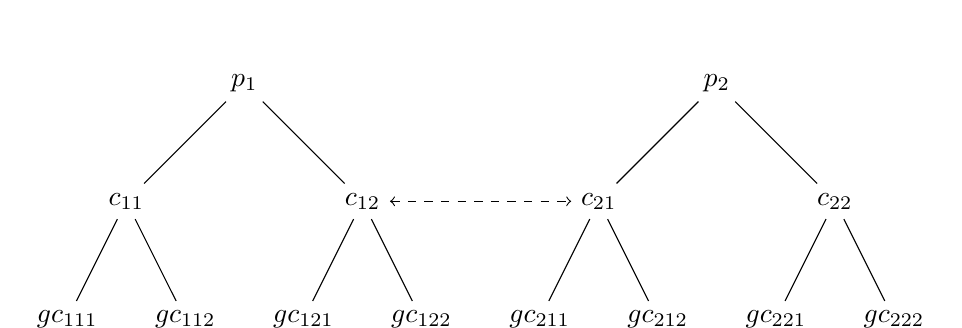
\begin{tikzpicture}[level distance=1.5cm,
            level 1/.style={sibling distance=3cm},
            level 2/.style={sibling distance=1.5cm}
        ]
        \node (p1) {$p_1$}
        child {node (c11) {$c_{11}$}
            child {node (gc111) {$gc_{111}$}}
            child {node (gc112) {$gc_{112}$}}
        }
        child {node (c12) {$c_{12}$}
            child {node (gc121) {$gc_{121}$}}
            child {node (gc122) {$gc_{122}$}}
        };
        \node[] at (6, 0) {$p_2$}
        child {node (c21) {$c_{21}$}
            child {node (gc211) {$gc_{211}$}}
            child {node (gc212) {$gc_{212}$}}
        }
        child {node {$c_{22}$}
            child {node (gc221) {$gc_{221}$}}
            child {node (gc222) {$gc_{222}$}}
        };
        \draw[dashed,<->] (c12) -- (c21);
    \end{tikzpicture}
    \caption[Cell lineage tree]{
        Arbitrary cells can not be interchanged freely since this might introduce incorrect
        configurations into the cell-lineage.
        For example, the two cousin-cells $gc_{212}$ and $gc_{221}$ would have different
        grandparent-cells if $c_{12}$ and $c_{21}$ would be interchanged.
    }
    \label{fig:cell-lineage-break}
\end{figure}

This exemplifies the need to assign unique identifiers for cells to correctly trace their lineage.
We call the set of all identifiers $J$ and only consider cells as a combination of an element
$c\in C$ with an identifier $\iota\in I$.
Thus a cell is an element of the product $J\times C$.
The explicit representation of $J$ can depend on the respective system in question.
To allow for processes such as cell-division and death we additionally must be able to treat a
variable number of cells throughout the evolution of the dynamical system.
The evolution function of our dynamical system will map cellular states onto each other, thus
acting on the cellular space $\CS$.
As can be seen from Figure~\ref{fig:cell-lineage-break}, division of cells introduces two new
identifiers for two new cells and consumes the previously existing cell.
Cell-death removes cells.
Newly inserted cells may not obtain previously used identifiers since this would again interfere
with cell lineage.
This means, we need to keep track of all identifiers $\iota\in I_p$ which have been used in the
past.

\begin{definition}[Cellular State]
    \label{def:cellular-state}
    Let $I$ be a set of identifiers and $C$ be the set describing cellular agents.
    We call a set of cells $(I_p,M)\in Pot(I)\times Pot(I\times C)$ a cellular state if
    \begin{enumerate}
        \item Every cell has a unique identifer $\#\pi_1(M)=\#M$.
        \item Identifiers have not been used previously $I_p\cap\pi_1(M)=\emptyset$
    \end{enumerate}
    where $\pi$ is the projection on the first component.
    The set $I_p$ contains identifiers which have been used previously.
\end{definition}

\begin{definition}[Cellular Space]
    \label{def:cellular-space}
    The cellular space $\CS(I, C)$ of an index set $I$ and cellular configuration space $C$
    is given by
    \begin{equation}
        \CS(I,C) = \{M\in Pot(I)\times Pot(I\times C) | M \text{ is cellular state }\}.
    \end{equation}
    We may choose the simplified notation $\CS = \CS(I, C)$ where the context is
    clear.
    We write $c_\iota:=(\iota,c)\in M$ where $(I_p,M)\in\CS$ despite the non-exhaustiveness
    of the index $\iota$ in a single cellular state.
\end{definition}

Cell division~\cite{bhlitem268752} is a process during which a cell transforms either via binary
(or multiple) fission~\cite{Biov2014} or mitosis~\cite{Ilowiecki1981,von1835resp} and
meiosis~\todo{CITATION} into separate
daughter cells.
To describe cell division, the dynamics behind this transition needs to be taken into account.
We will discuss this in the chapter~\ref{section:dynamics}.
In our agent-based approach, the end of this transition removes the old cell and inserts the new
daughter cells.

\begin{definition}[Single Cell Division]
    \label{definition:cell-division-single}
    We call a map $\gamma:C\rightarrow \cup_{n\geq 2}C^n$ a single division function and
    $\Upsilon:\{\gamma:C\rightarrow \cup_{n\geq 2}C^n\}\times I\times\CS\rightarrow\CS$ a
    single division operator if for any initial state $(I_p,M)\in\CS$ with $d_i\in M$ and
    final state $(J_p,N)=\Upsilon(\eta,i,(I_p,M))$
    \begin{enumerate}
        \item (Removal) Exactly one cell is removed $M\backslash N=\{d_i\}$
        \item (Insertion) At least two new cells are created:
            $N\backslash M=\{c_\iota,\tilde{c}_{\tilde{\iota},\dots}\}$
        \item (Tracking) We carry forward all old identifiers and the removed one:
            $J_p=I_p\cup\{i\}$
        \item (Uniqueness) New cells have new identifiers: $\iota,\tilde{\iota},\dots\notin J_p$.
    \end{enumerate}
    In the case when $i\notin\pi_1(M)$, we require $\Upsilon(\eta,i,(I_p,M))=(I_p,M)$.
    The last two conditions are to be thought of as one in order to guarantee uniqueness for each
    cell over the course of the total time of our system.
\end{definition}

\begin{definition}[Cell Division]
    \label{definition:cell-division-function}
    A division function $\gamma$ is the concatenation of single division functions
    $\{\gamma_i,i\in I\}$.
    We require that the overall effect is independent of the order of their individual applications,
    ie.
    \begin{equation}
        \prod\limits_{i_j\in I}\gamma_{i_j} = \prod\limits_{i\in I}\gamma_i
    \end{equation}
    where the product is with respect to the concatenation of maps.
\end{definition}

It is important to note that while this definition seems cumbersome in the first place, it is
essential in upkeeping a valid cellular state.
From an application standpoint, it is desirable to only specify the division map $\gamma$ and have
$\Upsilon$ be defined by the underlying modeling framework.

Any single-cell division function is only executed once the division process is completed and the
two new daughter cells can be identified.
To indicate the end of the division process a division criterion is used.

\begin{definition}[Cell Division Criterion]
    \label{definition:cell-division-criterion}
    A division criterion is a map $\bar{\gamma}:\mathscr{C} \rightarrow \{0,1\}$ which
    determines if the
    single division function~\ref{definition:cell-division-single} for the particular cell $c$ is
    realized.
\end{definition}

Another important process is that of cell death which is similarly as cell-division not instantanous
but occurs over a period of time.
Death schemes are categoritzed into programmed cell-death, also known as apoptosis~\cite{Kerr1965}
and necrosis~\cite{Gerschenson2001} which occurrs due to damage from external effects.
In principle, these processes take time in order to commence and the cell may interact with its
environment (ie. through secretion) during this stage.
Such transitions can be described by \todo{fill this} and will be discussed in
chapter~\ref{section:dynamics}.
Once the process of dying is over, the cell is removed.

\begin{definition}[Cell Removal]
    \label{definition:cell-death}
    % We call a map $\zeta:I_p\rightarrow \text{Pot}(I_p)$ a death-function
    Any cell-death removes a particular index $\iota\in I_p$.
    Thus the combination of many cell-daths is a mapping $\zeta:I_p\rightarrow \text{Pot}(I_p)$
    where $\text{Pot}(I_p)$ is the power set of $I_p$.

    \todo{
        - apoptosis
        - necrosis
        - removal
    }
\end{definition}

\begin{lemma}[Cell Lineage]
    \label{lemma:cell-lineage}
    Given an initial state $(I_p,M)\in\CS$, an arbitrary combination of applications of
    division and death functions creates a forest.
\end{lemma}
\begin{proof}
    We proof this statement via induction. For $n=0$ we are presented with a cellular state
    $M\in\CS$ which consists of cells $\{c_\iota\in M\}$.
    We interpret each cell as root of a new tree.
    In the induction step $n\rightarrow n+1$, we may assume that $G=(C,E)$ is a tree with
    cells as vertices.
    Any application of a division function $\Upsilon(\gamma, \dot)$ consumes a cell $c_{\iota_0}$
    and produces new cells $\{c_{\iota_1},\dots,c_{\iota_n}\}$.
    We thus insert the new cells as additional vertices with the edges
    $\{c_{\iota_0},c_{\iota_1}\},\dots,\{c_{\iota_0},c_{\iota_n}\}$.
    From the Uniqueness property of the cell-division
    definition~\ref{definition:cell-division-function},
    we know that the index of the removed cell $c_{\iota_0}$ will not occur for any further
    application of the division operator which means that the vertex of cell $c_{\iota_0}$ has $n$
    children.
    In the case of a death function, nothing happens.
    The associated cell $c_\iota$ will remain and endpoint for any further applications of death
    or division.
\end{proof}
\begin{corollary}[$k$-ary and Binary Cell Division]
    In the case where the single division function
    $\eta:C\rightarrow C^k\subset\cup_{n\in\mathbb{N}}C^n$
    is of k-ary nature, lemma~\ref{lemma:cell-lineage} retains a k-ary tree.
    The most common biological reality is the binary case.
\end{corollary}

%---------------------------------------------------------------------------------------------------
\subsection{Dynamics}
\label{section:dynamics}
\begin{definition}[Dynamical System]
    A dynamical system is a tuple $(T,M,\phi)$ where $T$ is a monoid (written additively) and
    $\phi$ is a mapping
    \begin{equation}
        \phi : U\subset(T\times M) \rightarrow M
    \end{equation}
    with $\pi_2(U) = M$ where $\pi_2$ is the projection on the second coordinate and $\phi$
    satisfies
    \begin{align}
        \phi(0,m) &= m\\
        \phi(t_2, \phi(t_1, m)) &= \phi(t_2+t_1,m).
    \end{align}
\end{definition}

We often write $\phi(t,m) = \phi_t(m)$.
The dynamics of \acp{abm} are governed by agents and their interactions with each other and the
simulation domain.
Thus we define our dynamical system to be of this shape.

\begin{definition}
    An \ac{abm} is a dynamical system which consists of a Cellular Space $\CS$ and a domain
    $\EV$.
    \begin{equation}
        M = \CS\times\EV
    \end{equation}
    Given an initial state $x_0$, we say that a cell $c$ with index $\iota$ is alive at point $t$ if
    $c_\iota\in\pi_1(\phi_t(x))$.
\end{definition}

It is of importance to consider the domain as an integral part of the dynamical system such that
interactions of the agents with it can permanently alter its constitution.
In this way, extracellular constituents can interact and change and even the overall spatial
configuration of the domain could be subject to dynamics.
Furthermore, we do not require that the monoid $T$ is a subset of the real numbers in order to allow
for discrete dynamical systems.
Furthermore, for simplicity we omit any Stochasticity from our system \todo{Can we fix this?}.
Practical applications which implement numerical routines should rely on pseudo-random number
generators which will produce deterministic results when given an initial seed.
By treating this initial seed as part of the initial values of our system, we are able to describe
pseudo-stochastic processes within a deterministic framework.

\todo{Define our dynamical system more precisely. What does it mean to be an index?
$\iota\in\phi_t$}

\begin{lemma}[Cellular Identity]
    \label{thm:cellular-uniqueness}
    Given an index $\iota\in I$ to an initial state $x$ of an \ac{abm}, we define the
    \textbf{Life-Span} of $\iota$ which is the set of all time-points for which the cell is alive
    \begin{equation}
        T_\iota=\{t\in T: c_\iota \text{ is alive}\}.
    \end{equation}
    If $T$ is an ordered and path-connected topological space, then $T_\iota$ is also
    path-connected.
    If $\mu$ is a measure on $T$, we also define the \textbf{Lifetime} with respect to this measure
    via
    \begin{equation}
        t_\iota:=\mu\left(T_\iota\right).
    \end{equation}
    In practial examples, $\mu$ will be given by the Lebesgue measure.
\end{lemma}
\begin{proof}
    Let $t<s\in T_\iota$ arbitrary.
    We pick a path $\gamma:[0,1]\rightarrow T$ from $t$ to $s$.
    Since $T$ is ordered, we can pick a path which satisfies $t\leq\gamma(h)\leq s$.
    By Definition~\ref{definition:cell-division-function}, properties 1 and 4, we see
    that every state
    between the points of insertion and removal are part of $T_\iota$ and thus
    $\gamma(h)\in T_\iota\forall h\in [0,1]$.
\end{proof}

%---------------------------------------------------------------------------------------------------
\subsection{Stochasticity}

%###################################################################################################
\newpage
\section{Applications}
%---------------------------------------------------------------------------------------------------
\subsection{Estimating Parameters of individual Rod-shaped bacteria}

\subsubsection{Motivation}
\textbf{List of problems}
\begin{itemize}
    \item varying number of vertices
    \item cell division leads to varying number of variables as well
    \item variable amount of datapoints is bad for optimization problems
    \item do both metrics provide the same optimal parameters (same minimum, maybe approximately)
    \item can we somehow reuse the position space metric for time-intervals of non-chaning topology?
        to reduce computational demand
    \item practical non-identifiability at division event in data; how can the position-space metric
        still provide relevant information?
\end{itemize}

\subsubsection{Computational Model}
\begin{itemize}
    \item only rely on discretization (at most); less assumptions is better
    \item
\end{itemize}

\subsubsection{Metrics: Position Space vs Image Space}
\begin{itemize}
    \item
\end{itemize}

\subsection*{Unsorted List of Ideas}
\begin{itemize}
    \item dynamical system factorizes through some subspace where we interchange the order and
        total number of vertices; this exchange is problematic for numerical
        implementations and only of theoretical nature
\end{itemize}

\subsubsection{Motivation}
\begin{itemize}
    \item mathematically motivate approach: compare simulation at points $\{t_i\}$ with data
    \item this requires us to compare all variables (positions, extracellular nutrients etc.)
    \item we need to be able to compare arbitrary states
    \item discuss strategies
        \begin{enumerate}
            \item compare positions in state1 with positions in state2; this does not work for
                celldivision
            \item if one state has more cells than other, assign arbitrary high cost
                function; this is
                poblematic since data for division is often incorrect/high uncertainty
            \item compare with cell masks and account for parental relationship; requires ancestor
                graph, this brings us back to the uniqueness in our previous section
        \end{enumerate}
    \item should account for parental relationship
    \item mathematically construct cost function
    \item take into account temporal component; at division event no cost for parents; then modify
        as difference to division event gets larger (this will yield a nice graph/figure)
    \item We should be able to further extend this approach into a metric which is
        measure-based instead of counting pixels.
        Even a probability measure could work. (probability of cell $\iota$ to be at this
        point, what about cell division?)
\end{itemize}

\subsubsection{Mathematical \& Computational Model}
\begin{itemize}
    \item Use contents from other paper
    \item show that this does not really depend on the underlying dynamics but rather only on the
        spatial representation
    \item perform all analysis with "generalized model for elongated bacteria"
    \item actually should also work for non-vertex approach (such as spline)
\end{itemize}

\subsubsection{Parameter Estimation: Defining a Cost Function}
\textbf{Formalize the notion of the comparison metric $d(x,y)$}
\begin{itemize}
    \item Consider the space $X$ which contains cell masks encoded by colors (maybe even
        3D possibly).
    \item we want to asses if the constructed mapping $d:X\times X\rightarrow X, d(x,y)$
        is a metric.
        \begin{enumerate}
            \item Distance to itself is zero: $d(x,x)=0$ \checkmark
            \item Positivity: $x\neq y$ then $d(x,y)$ will only be zero if the parent
                penalty $p$ is zero.
                If we introduce a time-dependent (monotonous) parent penalty $p(\Delta
                t)>0$ when $\Delta t>0$, we also retain this property.
            \item Symmetry: \checkmark
            \item Triangle inequality: This is true due to our individual treatment of
                cells and accounting for indices $\iota$.
                Suppose that we have $d(x,y) > d(x,z) + d(z,y)$ for a combination of $x,y,z$.
                Then this means that there is at least one pixel where the color value
                for $x,y$ are not matching but they are matching both for $x,z$ and $y,z$.
                This is equivalent to the fact that the associated color value of $z$ is
                the parent cell of $x$ and $y$ and can not be true since the parent index
                was removed.
        \end{enumerate}
    \item Therefore this is a true metric considering the restructions to $p(t)$ above.
\end{itemize}

\subsubsection{Relation to Identifiability Analysis}
Parameter estimation usually uses weighted sum of residuals
\begin{equation}
    \chi^2_\text{res}(p) = \sum\limits_{k=1}^m\sum\limits_{l=1}^{d_k}\left(\frac{y_{kl}^D
    - g_k(p,t_l)}{\sigma^D_{kl}}\right)
\end{equation}
where $\sigma_{kl}^D$ is the measurement error for datapoint $y_{kl}^D$ and time point $t_l$.
The most common estimator is the maximum likelihood estimator
\begin{equation}
    \tilde{p} = \text{arg min}\left[\chi^2_\text{res}(p)\right].
\end{equation}

\begin{definition}[Structural Identifiability]
    A model is \textit{structurally identifiable} if a unique parametrization exists for
    any given model output.
    A parameter $p_i$ is called \textit{globally structurally identifiable} if for every
    parameter vector $\textbf{p}$, it holds
    \begin{equation}
        y(p)=y(p') \Rightarrow p_i=p_i'.
    \end{equation}
\end{definition}

%---------------------------------------------------------------------------------------------------
\subsection{TODO find one more example for parameter estimation here}
\begin{itemize}
    \item \cite{Jin2022} 2 approaches: bottom-up and top-down, ("Studies of self-assembling systems
        have also benefited from top-down approaches.")
    \item \cite{Guenza2025} performance because of: less degrees of freedom; coarse-grained
        potentials are less steep
\end{itemize}

\subsection{Coarse-graining Ideas}

\begin{itemize}
    \item "The asymptotic coarse-graining formulation of slender-rods, bio-filaments and
        flagella Free"
        \url{https://doi.org/10.1098/rsif.2018.0235}
\end{itemize}

%---------------------------------------------------------------------------------------------------
\newpage
\subsection{Coarse-graining of an off-lattice center-based model}
This section formulates a generalized model for cellular dynamics, covering growth, division,
intracellular \& extracellular reactions and mechanical properties.
We assume that each cell is represented by a center-based, off-lattice point
$\textbf{x}_c\in\R^d$ and interacts in a
point-wise manner with the external environment.
This approach is general enough to cover a wide range of cellular systems while also providing the
necessary assumptions to derive meaningful results.
We model the system over the course of a time interval $I\subset\R$.
Within the model every alive cell $c\in\CS$ is described by an individual set of
equations for volume $V_c$, intracellular reactions $\textbf{v}_c$ and mechanics $\textbf{x}_c$.
These equations can be subject to heterogeneity and are thus not assumed to be identical in their
most generalized version.
Quantities which are specific to a particular cell $c\in\CS$ are indexed with said cell accordingly.
We will assume that all functions are sufficiently differentiable and that a solution to
the differential equations exists on $I$.
The system of equations is given by
\begin{alignat}{5}
    \partial_t{V_c} &= &&&&h_{g,c}(\textbf{v}_c, V_c)
    \label{eq:volumetric-growth}\\
    \partial_t{\textbf{v}_c} &=  &-&
    \textbf{T}_i\textbf{h}_x(\textbf{v}_c,\textbf{w}|_{\textbf{x}_c}) &+&
    \textbf{h}_{i,c}(\textbf{v}_c, V_c)
    \label{eq:intracellular-reactions}\\
    \partial_t{\textbf{w}} &= &\sum\limits_c \frac{V_c}{V_\EV}
    &\textbf{T}_e\textbf{h}_x(\textbf{v}_c,\textbf{w})\delta(\textbf{x}-\textbf{x}_c) &+&
    \textbf{h}_e(\textbf{w}) &+& \textbf{S}(\textbf{w})
    \label{eq:extracellular-reactions}\\
    % \partial_t \textbf{x}_c &= &\sum\limits_{s\neq c}&\textbf{G}(c,s) + \textbf{G}_\EV(c)
    % \label{eq:equations-of-motion-1}\\
    \partial^2_t\textbf{x}_c &= &\sum\limits_{s\neq c}& \textbf{F}_\CS(c,s) + \textbf{F}_\EV(c)
    \label{eq:equations-of-motion-2}\\
    &\gamma:&\CS&\rightarrow\CS\times\CS\\
    &\bar{\gamma}:&\CS&\rightarrow\{0,1\}.
\end{alignat}
\todo{Explain division functions}
Equation~\eqref{eq:volumetric-growth} defines the term $h_{g,c}(\textbf{v}_c, V_c)$ which
describes the rate of change of the volume of a single cell.
This growth term is coupled to the presence of intracellular concentrations
$\textbf{v}:I\rightarrow\R^n$.
Intracellular processes are expressed in equation~\eqref{eq:intracellular-reactions} via
$\textbf{h}_i(\textbf{v}_c, V_c)$ which also encompasses any growth-related changes.
We also model the dynamics of extracellular concentrations
(equation~\eqref{eq:extracellular-reactions})
$\textbf{w}:I\times\mathcal{D}\rightarrow\R^m$ which are distributed over the domain
$\mathcal{D}\subset\R^d$.
The integers $n,m$ refer to the number of intracellular/extracellular components
respectively while $d$ is the dimension of the physical environment (usually $d=2,3$).
The extracellular concentrations are coupled to the individual agents via an exchange
term $\textbf{h}_x(\textbf{v}_c,\textbf{w})$.
We have introduced two auxiliary diagonal matrices $T_i\in\R^{n\times l}$ and
$T_e\in\R^{m\times l}$ which enables us to utilize the same notion
$\textbf{h}_x(\textbf{v}_c,\textbf{w})$ for the intracellular $\textbf{v}_c$ and
extracellular $\textbf{w}$ derivative.
This choice ensures that extracellular and intracellular concentrations remain comparable
and tractable.
Since we have chosen to model concentrations, the exchange term
$\textbf{h}_x(\textbf{v}_c, \textbf{w})$ needs to be scaled with the ratio of cellular
volume $V_c$ to domain volume $V_\EV$ to correctly describe the total amount of exchanged resources.
The term $\textbf{S}(\textbf{w})$ is supposed to model transport of the extracellular compounds and
does not alter the total amount, i.e. $\int\textbf{S}(\textbf{w})\text{dV}=0$.
Table~\ref{table:overview-model-aspects} shows a summary of the model aspects that are treated with
this framework.
\begin{table}[h]
    \centering
    \renewcommand{\arraystretch}{1.2}
    \begin{tabular}{lclll}
        \toprule
        Model Aspect & Equation & Input && Output\\
        \midrule
        Growth Model            & $h_{g,c}(\textbf{v}_c,V_c)$               &
        $\R^n\times\R$    & $\rightarrow$ & $\R$\\
        Intracellular Reactions & $\textbf{h}_i(\textbf{v}_c,V_c)$          &
        $\R^n\times\R$    & $\rightarrow$ & $\R^n$\\
        Exchange                & $\textbf{h}_x(\textbf{v}_c, \textbf{w})$  &
        $\R^n\times\R^m$  & $\rightarrow$ & $\R^l$\\
        Extracellular Reactions & $\textbf{h}_e(\textbf{w})$                & $\R^m$
        & $\rightarrow$ & $\R^m$\\
        Fluid Motion            & $\textbf{S}(\textbf{w})$                  & $\R^m$
        & $\rightarrow$ & $\R^m$\\
        Mechanics               & $\partial_t^2\textbf{x}_c$                & $\R$
        & $\rightarrow$ & $\R^d$\\
        Division                & $\bar{\gamma},\gamma(c)$                  & $\CS$
        & $\rightarrow$ & $\CS\times\CS$\\
        \bottomrule
    \end{tabular}
    \caption[Dynamical Components of the center-based system]{Overview of terms
    contributing to the dynamics of the system.}
    \label{table:overview-model-aspects}
\end{table}

\subsubsection{Case 1: Full Reduction}
We consider the case with no cellular growth $h_{g,c}=0$, and aim to exclude any spatial
dependence by integrating over the domain $\EV$.
Furthermore, we assume that the dimensionality of intra- and extracellular reactions is
identical $n=m$ and that the exchange term is given by a fast linear term
$\textbf{h}_x~(\textbf{v}_c - \textbf{w})$.
These choices reduce the auxiliary matrices to $\textbf{T}_i=\textbf{T}_e=\mathbb{1}$.
Under the assumption that the exchange is fast compared the remaining processes, we can
assume that $\textbf{v}_c=\textbf{w}|_{\textbf{x}_c}$.
This considerably simplifies our system of equations leaving us with
\begin{equation}
    \partial_t\textbf{w} = \sum\limits_c
    h_{i,c}(\textbf{w}|_{\textbf{x}_c})\frac{V_c}{V_\EV}\delta(\textbf{x}-\textbf{x}_c) +
    \textbf{h}_e(\textbf{w}) + \textbf{S}(\textbf{w}).
\end{equation}
We integrate over the domain $\EV$ and obtain use the total amount of extracellular
compounds $\bar{\textbf{w}}:I\rightarrow\R^n$ instead of the previously used
concentrations $\textbf{w}$ to reformulate the resulting equation.
Carrying out these steps leads to
\begin{alignat}{7}
    \partial_t\bar{\textbf{w}} &=
    &\int\limits_\EV\sum\limits_c&
    \textbf{h}_{i,c}(\textbf{w})\frac{V_c}{V_\EV}\delta(\textbf{x} - \textbf{x}_c)\text{dV}
    &+& \bar{\textbf{h}}_e(\bar{\textbf{w}})
    &+& \int\limits_\EV\textbf{S}(\textbf{w})\text{dV}\\
    &= &\sum\limits_c& V_c\textbf{h}_{i,c}(\bar{\textbf{w}}) &+&
    \bar{\textbf{h}}_e(\bar{\textbf{w}})
    \label{eq:pool-model-case1-coarse-grained-result}
\end{alignat}
which is the direct combination of intra- and extracellular reactions.
Note that the final integral vanishes due to our assumptions that
$\textbf{S}(\textbf{w})$ only describes transport terms, leaving the total amount invariant.
The first term can be understood in terms of an expectation value $\text{E}(X_c)=\sum_c
X_c / N_\CS$ of a product of two distributions over living cells $c\in\CS$ which we will
use to rewrite equation~\eqref{eq:pool-model-case1-coarse-grained-result}.
In the general case where the distributions $V_c/V_\EV$ and
$\bar{\textbf{h}}_{i,c}(\bar{\textbf{w}})$ are not independent, we obtain
\begin{equation}
    \partial_t\bar{\textbf{w}} =
    N_\CS\text{E}\left(V_c\right)\text{E}(\textbf{h}_{i,c}({\bar{\textbf{w}}}))
    + N_\CS\text{Cov}\left(V_c,\textbf{h}_{i,c}({\bar{\textbf{w}}})\right)
    + \bar{\textbf{h}}_e(\bar{\textbf{w}})
\end{equation}

which can be further reduced, assuming that the distribution of volumes $V_c$ and
intracellular reactions is stochastically independent:
\begin{alignat}{5}
    \partial_t\bar{\textbf{w}} &=
    &N_\CS\text{E}\left(V_c\right)&\text{E}(\textbf{h}_{i,c}({\bar{\textbf{w}}}))
    &+& \bar{\textbf{h}}_e(\bar{\textbf{w}})\\
    &= &q& \textbf{h}_i(\textbf{w}) &+& \bar{\textbf{h}}_e(\bar{\textbf{w}})
\end{alignat}
We have used the expectation value to factorize the first term and $q=N_\CS\text{E}(V_c)$
with $\textbf{h}_i=\text{E}(\textbf{h}_{i,c})$ to simplify notation.
Using this concise notation, the final step shows that our equations reduce to a set of \acp{ode}.
The value $q$ is the fraction of total bacterial volume compared to the volume of the
domain $V_\EV$.

We can also reinterpret the sum in
equation~\eqref{eq:pool-model-case1-coarse-grained-result} via a continuous measure using
the probability to encounter a certain number of cells in the state $c\in C$.
For this reason it is desirable to omit the cellular identity at this point, thus
introducing the cellular density as a function $\rho:C\rightarrow\R$.
In the continuum limit, the sum transitions into an integral over the cellular
configuration space $C$ (see Section~\ref{subsec:cellular-space})
\begin{equation}
    \partial_t\bar{\textbf{w}}
    = \int\limits_C N_\CS\rho(c)\textbf{h}_{i,c}(\bar{\textbf{w}})\text{d}c
    + \bar{\textbf{h}}_e(\bar{\textbf{w}}).
\end{equation}

We can therefore interpret $\textbf{h}_{i,c}$ as a distribution of reaction functions and
the integral

\begin{equation}
    F[h_c] = \int\limits_C N_\CS\rho(c)h_c\text{d}c
\end{equation}

as an operator acting on this space.

\subsubsection{Case 2: With Exchange}
\textbf{TODO from here on the text has to adapted to the new expectation value formalism!}
We follow all steps identically to the previous case, but do not assume that the exchange
between intra- and extracellular compounds is fast resulting in
\begin{alignat}{3}
    \partial_t\bar{\textbf{v}}_c &= &- &\textbf{A}\left(\bar{\textbf{v}}_c -
    \frac{V_c}{V_\EV}\bar{\textbf{w}}\right) + \bar{\textbf{h}}_{i,c}(\bar{\textbf{v}}_c)\\
    \partial_t\bar{\textbf{w}} &= &\sum\limits_c&\textbf{A}\left(\bar{\textbf{v}}_c -
    \frac{V_c}{V_\EV}\bar{\textbf{w}}\right) + \bar{\textbf{h}}_e(\bar{\textbf{w}}).
\end{alignat}
We can see that in the case where nothing is exchanged $A=0$, the equations decouple.
Again utilizing the expectation value $\text{E}$, we can reformulate the equations and obtain
\begin{alignat}{5}
    \partial_t\text{E}(\bar{\textbf{v}}_c) &=
    &-& \textbf{A}\left(\text{E}(\bar{\textbf{v}}_c) -
    \text{E}\left(\frac{V_c}{V_\EV}\right)\bar{\textbf{w}}\right)
    &+& \text{E}\left(\bar{\textbf{h}}_{i,c}(\bar{\textbf{v}}_c)\right)\\
    \partial_t\bar{\textbf{w}} &=
    &&\textbf{A}\left(\text{E}(\bar{\textbf{v}}_c) -
    \text{E}\left(\frac{V_c}{V_\EV}\right)\bar{\textbf{w}}\right)
    &+& \bar{\textbf{h}}_e(\bar{\textbf{w}}).
\end{alignat}
With the transformations
\begin{align}
    \bar{\textbf{u}}_0 &= \text{E}(\bar{\textbf{v}}_c) - q\bar{\textbf{w}}\\
    \bar{\textbf{u}}_1 &= \text{E}(\bar{\textbf{v}}_c) + \bar{\textbf{w}}
\end{align}
and the substitutions
$\bar{\textbf{h}}_i=\text{E}(\bar{\textbf{h}}_{i,c}(\bar{\textbf{w}}))$ and
$q=N_\CS\text{E}(V_c/V_\EV)$, we obtain the system
\begin{alignat}{3}
    \partial_t\bar{\textbf{u}}_0 &= \bar{\textbf{h}}_i &-q& \bar{\textbf{h}}_e
    -(1+q)\textbf{A}\bar{\textbf{u}}_0 \\
    \partial_t\bar{\textbf{u}}_1 &= \bar{\textbf{h}}_i &+& \bar{\textbf{h}}_e
\end{alignat}
where the two equations are implicitly coupled due to the dependence of
$\bar{\textbf{h}}_{i/e}$ on $\textbf{u}_{0/1}$.

\subsubsection{Case 3: With Growth}
Now we will additionally consider the case where growth is introduced into the system via
equation~\eqref{eq:volumetric-growth}.
Growth of individual cells will lead to their division which can be defined by a division
function $\gamma:\CS\rightarrow\CS\times\CS$ and is executed when the division criterion
(see definition~\ref{definition:cell-division-criterion}) is satisfied $\bar{\gamma}(c)=1$.
This means that the sum over all cells $\sum_c$ depends on the current number of living
cells which is now a variable quantity.
Therefore, we introduce a new variable $V=\text{E}(V_c)=\sum_cV_c$.
We assume that any division event $\gamma(c)=(c_1,c_2)$ will lead to no loss or gain in
total volume $V_c=V_{c_1}+V_{c_2}$.
Therefore the dynamics of $N$ do not depend on $\gamma$ and $\bar{\gamma}$ but only on $h_{g,c}$.
We denote $\sum_c h_{g,c}=H_g$ and again do not consider any spatial distribution effects
or movement by the cells.
In addition we again assume fast exchange and obtain the equations
\begin{align}
    \partial_tV &= H_g(\textbf{w},V)\\
    \partial_t{\textbf{v}_c} &=  -
    \textbf{T}_i\textbf{h}_x(\textbf{v}_c,\textbf{w}|_{\textbf{x}_c}) +
    \textbf{h}_{i,c}(\textbf{v}_c, V_c)\\
    \partial_t{\textbf{w}} &= \sum\limits_c \frac{V_c}{V_\EV}
    \textbf{T}_e\textbf{h}_x(\textbf{v}_c,\textbf{w})\delta(\textbf{x}-\textbf{x}_c) +
    \textbf{h}_e(\textbf{w})\\
    \partial^2_t\textbf{x}_c &= \sum\limits_{s\neq c} \textbf{F}_\CS(c,s) + \textbf{F}_\EV(c)
\end{align}
%
%
\subsubsection{Case 4: Something Else}
Although the equations governing the \ac{abm} can not be derived directly from a higher
conceptual viewpoint, we are still able to motivate them and explain their individual components.
To this end, we consider the total energy stored in the system to be constant.
It is made up of the environment's energy and the energy stored within the cells, either
in the form of intracellular nutrients or converted into biomass.
This means that no additional nutrients are added and the existing energy is only
converted internally (i.e. from diffusive nutrients into cellular mass).
We denote the density of extracellular nutrients with $R_e$ and the intracellular
nutrients of species $A/B$ with $R_{i,c_{A/B}}$ respectively.
By integrating over the respective volumes and summing over all cellular agents, we
obtain the total amount of energy.
\begin{alignat}{5}
    \text{const}
    &=\int\limits_{V_D} R_e(x) \text{dVol} &+ \sum\limits_c\int\limits_{V_c}&R_{i,c}\text{dVol}\\
    &=\int\limits_{V_D} R_e(x) \text{dVol} &+ \sum\limits_c&R_{i,c}V_c
    \label{eq:supplement-abm-derivation-enthalpy-const}
\end{alignat}
We treat intracellular concentrations of nutrients $R_{i,c}$ as spatially homogenous
within each cell.
The resulting quantity can also be interpreted as the thermodynamic Enthalpy of the system.
It is usually defined as the product of pressure and volume but can expressed in terms of
the density when employing a linear equation of state relating pressure and density.
We postulate that this quantity stays constant.
From equation~\ref{eq:supplement-abm-derivation-enthalpy-const}, we can take the
derivative with respect to time and obtain
\begin{equation}
    0 =
    \int\limits_{V_D}\dot{R}_e(x)\text{dVol}
    + \sum\limits_c \left(\dot{R}_{i,c}V_c + R_{i,c}\dot{V}_c\right).
    \label{eq:supplement-abm-derivation-enthalpy-derivative}
\end{equation}
In order to link the extracellular nutrients $R_e$ to the intracellular ones $R_{i,c}$,
we add osmotic exchange terms of the forms
\begin{equation}
    \pm a
    \sum\limits_c\int\limits_{V_c}\frac{V_c}{V_D}\delta(x-x_c)(R_e(x)-R_{i,c})\text{dVol}
    = \pm a\sum\limits_c V_c (R_e(x_c)-R_{i,c})
    \label{eq:supplement-abm-derivation-osmotic-exchange-2}
\end{equation}
which are proportional to the difference of intra- to extracellular nutrient density.
In total we can now rewrite equation~\ref{eq:supplement-abm-derivation-enthalpy-derivative} to be
\begin{alignat}{7}
    0 &=
    \int\limits_{V_D}\dot{R}_e(x)\text{dVol}
    &-a\sum\limits_{c}&\int\limits_{V_{c}}&\frac{V_{c}}{V_D}&(R_e(x)-R_{i,c})\delta(x-x_{c})\text{dVol}&&
    \label{eq:supplement-abm-derivation-reactions-1}\\
    &&+ \sum\limits_{c}\Big[& &a&(R_e(x_{c})-R_{i,c}) V_{c} &+& \dot{R}_{i,c}V_{c} +
    R_{i,c}\dot{V}_{c}\Big]
    \label{eq:supplement-abm-derivation-reactions-2}
\end{alignat}
Upon closer inspection, we can now appreciate that the individual components of this
equation can be understood as spatially distributed processes (equation
\ref{eq:supplement-abm-derivation-reactions-1}) and intracellular processes respective to
individual cells \ref{eq:supplement-abm-derivation-reactions-2}.
We can ensure the conservation of energy be setting all of these components to zero
individually and requiring equality under the integral.
Additionally dividing by the volume $V_c$ of the cells for terms
\ref{eq:supplement-abm-derivation-reactions-2} and introducing diffusion for the
extracellular nutrients $R_e$ leads to
\begin{alignat}{3}
    \dot{R}_e(x) &=&-a\sum\limits_{c}\frac{V_{c}}{V_D}&(R_e(x)-R_{i,c})\delta(x-x_{c}) +
    D\Delta R_e(x)\\
    \dot{R}_{i,c} &= &+ a &(R_e(x_{c}) - R_{i,c_B}) -R_{i,c}\frac{\dot{V}_{c}}{V_{c}}
    \label{eq:supplement-abm-derivation-reactions-fin-2}
\end{alignat}
For the diffusive term $D\Delta R_e$, we assume Neumann boundary conditions such that no
extracellular nutrients $R_e$ are lost or gained via this process.
\begin{equation}
    \int\limits_D \Delta R_e(x) \text{dVol} = \int\limits_{\partial D} \nabla
    R_e(x)\text{d\textbf{A}}= 0
\end{equation}
It should be noted in particular that the terms
\ref{eq:supplement-abm-derivation-reactions-fin-2} are maintained within each individual
cell, not just on a global level.
Thus the system now consists of $1+N_A+N_B$ equations in total where $N_{A/B}$ are the
number of cells of species $A/B$ which changes (i.e. increases) over the course of the simulation.
We denote this fact and in general cell-specific properties with indices $c$ or $c_{A/B}$
if species-specific properties are at play.
In addition, we pick a growth model depending on the species $A/B$ of our cell
\begin{alignat}{3}
    \dot{V}_{c_A} &= &u \sigma &R_{i,c_A} V_{c_A}
    \label{eq:supplement-abm-derivation-growth-model-1}\\
    \dot{V}_{c_B} &= &\frac{u}{1+\nu_I I(x_{c_B})} \sigma &R_{i,c_B} V_{c_B}
    \label{eq:supplement-abm-derivation-growth-model-2}
\end{alignat}
which is proportional to the total cellular nutrients given by the product of the
intracellular nutrient density $R_{i,c}$ and its volume $V_c$.
Equation \ref{eq:supplement-abm-derivation-growth-model-2} is modulated by the abundance
of an extracellular inhibitor resource $I(x)$ whose dynamics are not yet specified.
However, these dynamics do not play any role for our the conservation law as it only
controls the rate of the growth.
The two factors $a,\sigma$ represent the rate with which the intracellular nutrients are
depleted and the conversion factor which turns nutrients into cellular volume respectively.
%
%
\vfill
\pagebreak
\subsubsection{Case 5: Pool Model Considerations}
\label{sec:supplement-abm-derivation}
The equations governing the dynamics of the \ac{abm} can not be directly derived from
higher principles but can still aim to motivate them as best as possible.
Our model consists of individual cells with volume $V_c$ and extracellular nutrients
$R_e(x)$ which are spatially distributed.
We set up a balancing equation that aims to relate these concepts.
To this end, we assume that any loss in extracellular nutrients is directly converted
into cellular volume.
To compare any changes in $R_e$ with changes of volume, we introduce a conversion factor $\sigma$.
The balancing equation then reads
\begin{equation}
    \text{const} = \sigma \int\limits_D R_e(x)\text{dVol} + \sum\limits_c V_c.
\end{equation}
We now assume that there are two species $A,B$ present and split the sum and since we are
interested in the dynamics of the system, we also take the temporal derivative.
By adding a zero in the form of
\begin{equation}
    \pm u_c\sigma \sum\limits_c\int\limits_D\frac{V_c}{V_D}R_e(x)\delta(x-x_c)\text{dVol}
\end{equation}
we can introduce an exchange term between extracellular nutrients and cellular volume.
In total we obtain
\begin{alignat}{3}
    0 &= \sigma\int\limits_D\dot{R}_e(x)\text{dVol} &+ \sigma\sum\limits_c
    u_c&\int\limits_D\frac{V_c}{V_D}R_e(x)\delta(x-x_c)\text{dVol}\\
    &&- \sigma\sum\limits_c
    u_c&\int\limits_D\frac{V_c}{V_D}R_e(x)\delta(x-x_c)\text{dVol} + \sum\limits_c \dot{V}_c\\
    &= \sigma\int\limits_D\Big[\dot{R}_e(x) &+ \sum\limits_c
    u_c&\frac{V_c}{V_D}R_e(x)\delta(x-x_c)\Big]\text{dVol}
    \label{eq:supplement-abm-derivation-intermediate-3}\\
    &&- \sum\limits_c\Big[\sigma u_c&V_cR_e(x_c) + \dot{V}_c\Big].
    \label{eq:supplement-abm-derivation-intermediate-4}
\end{alignat}
In order to satisfy this balancing equation, we can enforce equality of the dynamics for
the subsystems given by \ref{eq:supplement-abm-derivation-intermediate-3} and
\ref{eq:supplement-abm-derivation-intermediate-4}.
These can be viewed as the extracellular dynamics surrounding the nutrient resource $R_e$
and intracellular dynamics increasing the volume $V_c$.
We assume that the spatial distribution of $R_e$ is governed by a diffusion process with
Neumann boundary conditions such that no additional nutrients are introduced and no nutrients lost.
In particular, any diffusion effects vanishe in the integral
\begin{equation}
    \int\limits_D\Delta R_e(x)\text{dVol} = \int\limits_{\partial D}\nabla
    R_e(x)\text{d\textbf{A}} = 0
\end{equation}
due to the Neumann boundary conditions.
We separate the preceding equations and enforce equality of the dynamics under the integral.
We therefore obtain
\begin{align}
    \dot{R}_e(x) &= -\sigma\sum\limits_c u_c\frac{V_c}{V_D}R_e(x)\delta(x-x_c) + D_R\Delta R_e(x)\\
    \dot{V}_c &= \sigma u_c R_e(x_c)V_c
\end{align}
where $D_R$ is the diffusion constant of the nutrients $R_e$.
So far, we have treated all cells equally but the system which we aim to describe
consists of two distinct species $A/B$ which behave differently.
We can express this variation by introducing differing growth terms $u_c$ depending on the species.
This splits apart the sum, raning over cells $c_A$ and $c_B$.
Another mechanism of this system is the inhibition of growth mediated by an external
inhibitor $I$ which is produced by species $A$.
We assume that the release of inhibitor molecules can be neglected for the assumptions
governing the initial balancing of the system.
In addition to the production of the inhibitor, we also introduce diffusion with constant
$D_I$ which results in
\begin{equation}
    \dot{I}(x) = b\sum\limits_{c_A}\frac{V_{c_A}}{V_D}\delta(x-x_{c_A}) + D_I \Delta I(x).
\end{equation}
By splitting up all terms with respect to species, we arrive at our final equations
\begin{alignat}{5}
    \dot{V}_{c_A} &= &\sigma u& R_e(x_c)V_c\\
    \dot{V}_{c_B} &= &\sigma \frac{u}{1+\nu I(x_{c_B})}&R_e(x_{c_B})V_c\\
    \dot{R}_e(x) &=
    &-\sigma u&\sum\limits_{c_B}\frac{V_{c_B}}{V_D}R_e(x)\delta(x-x_{c_B})\\
    &&-\sigma\frac{u}{1+\nu I(x_{c_B})}&\sum\limits_{c_B}
    \frac{V_{c_A}}{V_D}R_e(x)\delta(x-x_{c_B}) &+& D_R\Delta R_e(x)\\
    \dot{I}(x) &= &b&\sum\limits_{c_A}\frac{V_{c_A}}{V_D}\delta(x-x_{c_A}) &+& D_I \Delta I(x).
\end{alignat}

\subsubsection{Case 6: Constant Enthalpy}
\begin{itemize}
    \item postulate that enthalpy should be constant
    \item show how the coupling of intracellular with extracellular components leads to the
        equations which we provided above
    \item the dimensions of the equations below do not match. Either make assumption on matrices $T$
        or somehow resolve this.
    \item what is enthalpy? what does this mean for biological systems?
        biological systems are basically always out of equilibrium. How does this compare?
\end{itemize}

Energy conservation
\begin{equation}
    \text{const} = \int\limits_\EV \textbf{w} \text{dVol} + \sum\limits_c V_c \textbf{v}_c
\end{equation}
Take derivative
\begin{equation}
    0 = \int\limits_\EV \partial_t\textbf{w} \text{dVol} + \sum\limits_c \partial_t V_c
    \textbf{v}_c + V_c \partial_t\textbf{v}_c
\end{equation}

% With these assumptions, we again
% \begin{alignat}{5}
%     \dot{R}_e(x) &=
%         &-u\sum\limits_{c_A}\frac{V_{c_A}}{V_D}&R_e(x)\delta(x-x_{c_A}) &+& D_R\Delta R_e(x)\\
%     \dot{R}_{i,c_A} &= -u\sigma R_{i,c_A}^2 &+ u &R_e(x_{c_A})V_{c_A}\\
%     \dot{R}_{i,c_B} &= -u\sigma R_{i,c_B}^2 &+ \frac{u}{1+\nu_I I(x_{c_B})} &R_e(x_{c_B})V_{c_B}\\
%     \dot{V}_c &= u \sigma R_{i,c} V_c\\
%     \dot{I}(x) &=&b\sum\limits_{c_A}\frac{V_{c_A}}{V_D}&\delta(x-x_{c_A}) &+& D_I\Delta I(x)
% \end{alignat}
%
%

%---------------------------------------------------------------------------------------------------
\newpage
\subsection{The Fractal Structure in Branching Patterns of \textit{Bacillus Subtilis}}
We set out to derive a set of equations to describe a simple bacterial system which grows
spatially by taking up nutrients.

\begin{itemize}
    \item PDE models of bacterial branching \cite{Kawasaki1997,Matsushita1998}
\end{itemize}

\begin{alignat}{5}
    \dot{n} &= &&\nabla^2n &- &f(n, b)\\
    \dot{b} &= d&&\nabla^2b &+ \theta &f(n, b)
\end{alignat}
The function $f(n,b)$ describes the nutrient consumption by the bacterial metabolism and $d$ is the
ratio of diffusion constants.

\begin{table}[h]
    \centering
    \def\arraystretch{1.5}
    \begin{tabularx}{\textwidth}{cllX}
        & \textbf{Modeling Aspect} & \textbf{Description} & \\
        \midrule
        (C) & Mechanics & Damped Newtonian &
        $m \ddot{\textbf{x}}_c = \textbf{F} - \lambda \dot{\textbf{x}}_c$\\
        (C) & Intracellular Reactions & Volumetric Growth & $\dot{V}_c = \alpha u n_e(x_c)$\\
        (C) & Cycle & Division & Division when radius exceeds threshold $r\geq r_\text{thresh}$\\
        (CC) & Physical Interaction & Morse Potential &
        $U(r) = U_0 \left(1- e^{-\beta (r-R)} \right)^2$\\
        (EC) & Extracellular Reactions & Diffusion, Uptake &
        $\dot{n}_e(x) = D\Delta n_e - u \sum_c n_e(x)\delta(x-x_c)$\\
        \bottomrule
    \end{tabularx}
    \caption[Simulation Aspects of Bacterial Branching]{\todo[inline]{add caption}}
\end{table}

\paragraph{Coarse-Graining}
Combine multiple cells into one circle \cite{Graham1998}

\begin{figure}[h]
    \centering
    \begin{tikzonimage}[width=0.158\textwidth]
        {figures/abm-theory/sim-branching/diffusion-80/discretization-nvoxels-000666.png}
        \node at (0.025, 0.975)[anchor=north west, rectangle, draw, white, minimum
        width=14pt, minimum height=14pt]{\textbf{A}};
    \end{tikzonimage}%
    \hspace{0.01\textwidth}%
    \begin{tikzonimage}[width=0.158\textwidth]
        {figures/abm-theory/sim-branching/diffusion-80/discretization-nvoxels-000080.png}
        \node at (0.025, 0.975)[anchor=north west, rectangle, draw, white, minimum
        width=14pt, minimum height=14pt]{\textbf{B}};
    \end{tikzonimage}%
    \hspace{0.01\textwidth}%
    \begin{tikzonimage}[width=0.158\textwidth]
        {figures/abm-theory/sim-branching/diffusion-80/discretization-nvoxels-000042.png}%
        \node at (0.025, 0.975)[anchor=north west, rectangle, draw, white, minimum
        width=14pt, minimum height=14pt]{\textbf{C}};
    \end{tikzonimage}%
    \hspace{0.01\textwidth}%
    \begin{tikzonimage}[width=0.158\textwidth]
        {figures/abm-theory/sim-branching/diffusion-80/discretization-nvoxels-000029.png}%
        \node at (0.025, 0.975)[anchor=north west, rectangle, draw, white, minimum
        width=14pt, minimum height=14pt]{\textbf{D}};
    \end{tikzonimage}%
    \hspace{0.01\textwidth}%
    \begin{tikzonimage}[width=0.158\textwidth]
        {figures/abm-theory/sim-branching/diffusion-80/discretization-nvoxels-000022.png}%
        \node at (0.025, 0.975)[anchor=north west, rectangle, draw, white, minimum
        width=14pt, minimum height=14pt]{\textbf{E}};
    \end{tikzonimage}%
    \hspace{0.01\textwidth}%
    \begin{tikzonimage}[width=0.158\textwidth]
        {figures/abm-theory/sim-branching/diffusion-80/discretization-nvoxels-000017.png}
        \node at (0.025, 0.975)[anchor=north west, rectangle, draw, white, minimum
        width=14pt, minimum height=14pt]{\textbf{F}};
    \end{tikzonimage}\\
    \begin{tikzonimage}[width=0.33\textwidth]
        {figures/abm-theory/fractal-dim-box-size-scaling.pdf}
        \node at (0.025, 0.975)[anchor=north west, rectangle, draw, minimum width=14pt,
        minimum height=14pt]{\textbf{G}};
    \end{tikzonimage}%
    \begin{tikzonimage}[width=0.33\textwidth]
        {figures/abm-theory/fractal-dim-vs-diffusion-constant.pdf}
        \node at (0.025, 0.975)[anchor=north west, rectangle, draw, minimum width=14pt,
        minimum height=14pt]{\textbf{H}};
    \end{tikzonimage}%
    \begin{tikzonimage}[width=0.33\textwidth]
        {figures/abm-theory/fractal-dim-over-time.pdf}
        \node at (0.025, 0.975)[anchor=north west, rectangle, draw, minimum width=14pt,
        minimum height=14pt]{\textbf{I}};
    \end{tikzonimage}
    \caption[Evaluations of the fractal dimension for a bacterial branching system]{
        (A-F) Calculation steps for determining the fractal dimension for varying number of voxels
        $N_v\in\{666,80,42,29,22,17\}$ for $D=80\SI{80}{\second^2\per\micro\metre^2}$.
        (G) Double-logarithmic plot of number of occupied voxels againts their size.
        The linear slope determines the fractal dimension of the structure.
        (H) Fractal dimension as a function of the diffusion constant of the nutrients.
        (I) Temporal evolution of fractal dimension.
    }
\end{figure}

\begin{itemize}
    \item combine multiple circles $k$
    \item volume $V_k = k V_0$ and $\dot{V}_k = k V_0$
    \item mass $m_k = k m_0$
    \item radius $R_k$
    \item interaction $U(r)= \sum U_0 (1-e^{-\beta(r-R)})^2$
    \item extracellular $\dot{n}_e(x) = D\Delta n_e - uk\sum_c n_e(x)\delta(x-x_c)$
\end{itemize}

\begin{itemize}
    \item show that we again obtain a branching simulation
    \item some parameters are scaled with $k$ determine their functional dependence
\end{itemize}

\begin{figure}
    \centering
    \begin{tikzonimage}[width=0.33\textwidth]
        {figures/abm-theory/morse-potential.pdf}
        \node at (0, 1)[anchor=north west, rectangle, draw, minimum width=14pt, minimum
        height=14pt]{\textbf{A}};
    \end{tikzonimage}%
    \begin{tikzonimage}[width=0.66\textwidth]
        {figures/abm-theory/circle-packing.pdf}
        \node at (0, 1)[anchor=north west, rectangle, draw, minimum width=14pt, minimum
        height=14pt]{\textbf{B}};
    \end{tikzonimage}
    \caption[Coarse-graining of the interaction potential]{
        (B) Coarse-graining approach of combining multiple cells into one larger one.
        It was shown that these packings are optimal by maximizing the density.
        The last three configurations have only been conjectured so far.
    }
\end{figure}

\paragraph{Research Steps}
\begin{enumerate}
    \item is it possible to construct a \ac{ode} which describes the relation:
        \begin{align}
            \frac{\partial \textbf{p}_k}{\partial k} &= \textbf{f}(\textbf{p}_k)\\
            \textbf{p}_{k=1} &= \textbf{p}_0
        \end{align}
    \item possibly we need to modify the approach from above and formulate it in terms of the
        objective function $\Omega$
        \begin{equation}
            \frac{\partial\Omega}{\partial k} = F(k)
        \end{equation}
    \item Maybe it is also more interesting to describe a relation with a different methodology, not
        as a differential equation, explore this
\end{enumerate}

%---------------------------------------------------------------------------------------------------
\newpage
\subsection{Cell Sorting}

\begin{itemize}
    \item \cite{Volfson2008} TODO; continuum model, equations of nematodynamics \cite{Doi1988-ad}
    \item \cite{Joshi2019} "The interplay between activity and filament flexibility determines the
        emergent properties of active nematics"
    \item \cite{Jin2020} "Influence of cell interaction forces on growth of bacterial biofilms"
    \item \cite{Ingham2008} "Swarming and complex pattern formation in Paenibacillus vortex studied
        by imaging and tracking cells"
\end{itemize}

%---------------------------------------------------------------------------------------------------
\subsection{Elementary CA}

\chapter{Parameter Estimation, Model Validation \& Reduction for Mechanical Models of
Elongated Bacteria}

\epigraph{No life is worth living if we cannot be true to our nature.}
{\textit{Baine Bloodhoof}}

\section*{Abstract}
Elongated bacteria such as \acl{ecoli} and \acl{bsubtilis} possess distinct mechanical
and physiological properties that shape their growth, division, and collective behaviors.
Despite the importance of these organisms, existing computational frameworks rarely capture their
flexible filamentous morphology, limiting the ability to study their mechanics in a systematic and
quantitatively grounded way.
Agent-based models are well suited for representing individual cells and their interactions, yet
their application to flexible rod-shaped bacteria has been hindered by the absence of appropriate
mechanical formulations and by the lack of practical methods for estimating model parameters from
experimental data.
In this work, we introduce a computational model that represents elongated bacteria as deformable
rods capable of growth, elastic bending, and mechanical interactions.
We develop a novel set of imaging- and geometry-based methods that extract cell shape and positional
information from segmented microscopy data and quantitatively compare it with model simulations at
the single-cell level.
These methods allow for a detailed analysis of the underlying dynamics of the model.
They allow us to apply maximum-likelihood and profile-likelihood estimation techniques to determine
the parameters of the underlying model.
We apply them across multiple experimental scenarios of increasing complexity, including cases that
exhibit substantial cell-cell variability and show how these methods can be used to perform model
validation and reduction.
Our results demonstrate that direct parameter estimation with cellular heterogeneity for complex
agent-based models of bacteria is feasible and can yield biologically interpretable constraints on
cellular parameters.
The developed are readiliy available as a modular Python package backed by a high-performing backend
written in Rust and integrate into our previously devleped agent-based simulation framework
\texttt{cellular\_raza}.

\section*{Author summary}

% \pagebreak
% \renewcommand{\contentsname}{Table of Contents (remove before submission)}
% \tableofcontents
% \vfill
\pagebreak

% \begin{itemize}
%     \item Adapt introduction; \acp{abm} not focus of paper, but rather tool to do the job
%     \begin{itemize}
%         \item model division, growth of bacteria
%         \item \acp{abm} are good for this tool
%     \end{itemize}
%     \item Exchange $\sigma \rightarrow R_1+R_2$
%     \item Equation 8 make double norm $||\vec{F}||$
%     \item Remove auxiliary variable $\vec{F}$ only use $\vec{\nabla}V$
%     \item Table 2 in supplement? (probably not)
%     \item numerical implementation verschieben?
%     \item numerical implementation: waht do we need to simulate this?
%     \begin{itemize}
%         \item \acp{abm} are common tools to realize this
%         \item cellular\_raza is THE tool to do it
%     \end{itemize}
%     \item Methodology: single-cell parameter estimation as motivation for techniques
%     \item Which parameters are global which are individual? Discuss this in general; not in detail
%     \item depends on data, number of parameters (computational efficiency)
%     \item page 12; yes this is Discussion
%     \item page 12: maybe extend the paragraph wrt comparison in intervals
% \end{itemize}

%###################################################################################################
\section{Introduction}

% \begin{itemize}
%     \item Problem 1: How to model flexibel rods and validate these models?
%     \begin{itemize}
%         \item Flexible rods so far only covered in soft-matter studies; rarely applied in direct
%             biological contexts
%         \item \acp{abm} are \textit{the} tool to use for individual-based modeling (combine with
%             reactions, cell cycle, division, differentiation, etc.)
%     \end{itemize}
%     \item Problem 2: How to estimate parameters for individual-based models of cells/bacteria
%     \item Problem 3: How to incorporate division and heterogeneity in parameter estimation?
%
%     \item Literature Gap 1: No \acp{abm} support flexible elongated bacteria
%     \item Literature Gap 2: Noone really does parameter estimations
%     \item Literature Gap 3: Cellular heterogeneity sometimes accounted for in simulation but not
%         in parameter estimation
%
%     \item Why matter 1: No explainability without parameters
%     \item Why matter 2: How can we be sure to actually model biological reality?
%     \item Why matter 3: Bacteria especially elongated are fundamental. Understanding them is
%         important.
%
%     \item What we do 1: Construct new mechanical model for rod-shaped bacteria
%     \item What we do 2: Develop methods to compare numerical results with data
%     \item What we do 3: Apply these methods in 3 scenarios covering different aspects
%
%     \item Why contribution significant 1: Show that parameter estimation can be done
%     \item Why contribution significant 2: Show how to treat heterogeneity and that we can map 1:1
%         of model to cells
%     \item Why contribution significant 3: New model for flexible rods which integrates in
%         \texttt{cellular\_raza} and can thus be readily reused by researchers
% \end{itemize}

Bacteria come in various shapes~\cite{Young2006,Young2007}, ranging from simple spheres to complex
spirals and helices.
Elongated bacteria form an important subclass that includes some of the most studied model
organisms such as \ac{ecoli} or \ac{bsubtilis}.
Their filamentous structure underlies distinct mechanical~\cite{Daniel2003} and physiological
constraints~\cite{Jones2001}, thus influencing other cellular aspects such as
growth~\cite{Chang2014} and division~\cite{Li2007}.
It also facilitates processes such as swarming~\cite{Harshey1994} or biofilm
formation~\cite{Duvernoy2018}.

Computational methods can allow for a systematic analysis of the underlying biological reality.
To this end, \acp{abm} provide a natural way of mapping cellular processes to computational
routines.
By treating cells as individual entities with their own state, these tools enable researchers to
think in terms of cellular properties and processes, thereby allowing for a mechanistic
understanding of the system.
This bottom-up perspective has transformed the analysis of complex cellular
systems~\cite{Pleyer2023} over a wide range of
topics~\cite{Ghaffarizadeh2018,Cooper2020,Karolak2021,DeRybel2014}.
\acp{abm} are generally capable of incorporating gene regulatory networks, cell cycle, division,
differentiation, transport of extracellular compounds and many other processes which makes them the
ideal tool to study the individual behavior of cells.

We develop a new agent-based computational model for flexible, elongated bacteria which
is a mechanical feature that is absent in most \acp{abm}.
So far, only a few computational studies have considered flexible rods~\cite{Duman2018,Joshi2019},
but their models cannot be transferred directly to more complex biological systems which might
involve intracellular reactions, extracellular compounds, growth and division.
Only a few \acp{abm} support even the less complex cylindrical
shapes~\cite{Kang2014,Breitwieser2021,Gorochowski2012} but none are able to capture
flexible filamentous bacteria.
This poses a problem in the computational study of these systems.

Although \acp{abm} seem destined to be applied to the modeling of individual elongated bacteria,
this potential has not been fully realized yet.
Another major problem is how to perform parameter estimations for \acp{abm}.
Classical approaches in systems biology include techniques such as maximum
likelihood~\cite{Kreutz2013,Raue2014} or maximum a posteriori estimation, identifiability analysis
and model reduction~\cite{Simpson2025,Gbor2015,Banga2008,Ashyraliyev2009}.
While some attempts have been made to properly calibrate the \ac{abm} at hand and estimate its
parameters~\cite{An2016,Lima2021,Dancik2010,Thiele2014} these methods are not widely applied and are
generally not used to explicitly capture any possible heterogeneity within the cellular population.
However, this can leave important questions unanswered:
Which combination of parameters drive the observed phenomena?
Can these parameters be identified given a set of datapoints?
Is there a simpler, i.e. reduced model that can describe the same phenomena?
If \acp{abm} are not able to answer these questions, their results will significantly lack in
explanatory power and their ability to link to the specific problem at hand.

The aforementioned problems present significant gaps in the scientific literature.
First, no model can be explained or interpreted without knowing the roles and values of its
parameters or how they are constrained.
Furthermore, models which are not properly calibrated, i.e. by a data-based approach or via
domain-specific knowledge, cannot guarantee to accurately represent the underlying
biological reality.
Finally, elongated bacteria are fundamental organisms which can be seen as a precursor to
more complex shapes such as spiral bacteria.
Obtaining a mechanistic understanding of their mechanical properties is essential to understand
emergent phenomena such as the formation of biofilms~\cite{Li2025} or bacterial
swarming~\cite{Starru2007}.

In this work, we address these challenges with the aim to further close the previously identified
gaps.
We provide a framework that links mechanistic modeling of elongated bacteria with quantitative
analysis methods (Figure~\ref{fig:flowchart-project-structure}).
First, we construct a novel mechanical model for flexible, elongated bacteria that captures growth,
division, elastic deformations of the rod and mechanical interactions between cells.
Second, we develop computational methods which utilize segmented microscopic images to
quantitatively
compare numerical results with biological data on the single-cell level.
With these methods we can estimate the parameters of our model in three scenarios, each probing
different aspects of our model with increasing levels of complexity.

A key feature of this framework is its modularity.
While most subcomponents (see Figure~\ref{fig:flowchart-project-structure}) rely on the spatial
representation of bacteria as discretized vertices, others i.e. the
\nameref{subsec:image-space-metric} operate purely on segmentation masks, making them fully
model-agnostic.
This enables researchers to freely reuse our developed methods across a wide range of models for
elongated organisms.

Our approach demonstrates that parameter estimation of \acp{abm} is indeed feasible, even in
the case of complex models such as single-cell modeling of flexible elongated bacteria and when
incorporating cellular heterogeneity.
The developed methods fill a methodological gap and present a novel way of fitting individual-based
models to data which can be readily adapted to various other scenarios.
Our novel mechanical model for flexible elongated bacteria integrates seamlessly into our previously
developed agent-based modeling framework \texttt{cellular\_raza}~\cite{Pleyer2025}.
It is purposefully designed to provide a flexible platform without any particular assumptions on the
cellular representation or the nature of their processes.
This allows researchers to freely adapt the underlying cellular model to their needs and enables
further usage of the presented approach in future studies.
In total, these contributions push for a more rigorous, interpretable and biologically grounded
development process for \acp{abm} which provide deeper mechanistic insights into the nature of
cellular behaviors.

%###################################################################################################
% \section{Overview}
% This work consists of many subcomponents which can be combined in order to achieve various tasks.
% Figure~\ref{fig:flowchart-project-structure} shows a high-level overview of all components.
% We assume that bacterial rods can be represented by a colleciton of vertices (see
% section~\ref{subsec:spatial-representation}).
% This assumption alone is enough to enable a cascade of other components.
% Using the spatial representation, we provide visualization methods that employ a 3D rendering
% engine and can produce cell masks or rendered images from a given configuration.
% The data extraction component determines the vertices from given segmented microscopic images.
% This allows us in particular to turn any sequence of images (movie) into a sequence of bacterial
% positions and is a key feature of the parameter estimation methods.
% The dynamics of the vertices are determined by a computational model which is specific
% to the respective use-case and should be defined by the researcher.
% It merely requires the aforementioned assumption of representing bacterial rods as a
% collection of vertices.
% This work will provide one example of how such a model can be defined.
% Notably, the visualization and data extraction components do not require any knowledge about the
% computational model, thus allowing us to reuse their functionality across differing models.
%
% By utilizing the provided data extraction methods, we can infer properties of the
% bacteria that aid
% us in constructing a suitable computational model.
% However, the construction of any mechanistic model also requires prior konwledge which can be used
% to inform our analysis methods.
% For example, by extracing the positions of bacteria across a time-series of microscopic images, we
% can also calculate their lengths at these time-points and thus determine their rate of growth and
% type of growth (see \nameref{paragraph:parameter-estimation-individual-treatment}), thus
% effectively guiding our modeling steps.
% As we will show later, extracted data in the form of cellular positions or segmentation masks can
% also be used for comparing computational results with biological ground truth.
%
% Visualization methods are an integral part of any modeling endevaour.
% They allow researchers to obtain feedback quickly and improve iteration times when
% constructing new
% models.
% Furthermore, we utilize them in our image-space metric (see
% section~\ref{subsec:image-space-metric}) where they enable us to effectively compare
% two bacterial configurations while accounting for division events.
% In the future, we are planning to extend the the rendering capabilities of our approach and
% generate realistic microscopic images and time-series.
% Together with the parameter estimation methods, they can then be used to provide large amounts of
% mechanistic data for the training of cell-segmentation and cell-tracking machine-learning
% algorithms.

\begin{figure}[H]
    \centering
    % \includestandalone[width=0.8\textwidth]{figures/cr_mech_coli/concept/overview}
    \caption{
        Modular framework for parameter estimation of elongated bacteria.
        The framework relies on a unified spatial representation (left) which discretizes
        bacteria into vertices.
        Building on top are visualization methods (top), a novel computational model for flexible
        elongated bacteria (middle) and data extraction routines (bottom).
        Analysis methods (bottom right) utilize extraction methods and can be informed by the model
        or used to guide modeling choices.
        The parameter estimation module integrates the preceding ones and allows us to calibrate the
        model which can then be used in generating synthetic data (top right).
        Colors indicate the component type; core scientific drivers (red), auxiliary
        methods (yellow)
        and extensions (blue).
    }
    \label{fig:flowchart-project-structure}
\end{figure}

%###################################################################################################
\section{A Computational Model for Rod-Shaped Bacteria}
\label{sec:computational-model}

The mechanical behavior of rod-shaped bacteria is governed by a plethora of effects.
In this work, we aim to establish a model which is general enough such that it can be reused as the
basis for many variants of rod-shaped bacteria but also explicit enough such that we can quantify
its parameters.
We thus utilize only a minimal set of assumptions.
When describing the bacterial system, we distinguish between intra-cellular processes and cell-cell
interactions.
We restrict ourselves to the features discussed below and summarize them in
Table~\ref{table:simulation-aspects}.

While some rod-shaped bacteria grow by inserting new material at the ends, \ac{ecoli} and
\ac{bsubtilis} utilize a method where new material is inserted along the cylindrical part of
the rod. The details of the division event (i.e. Z-Ring formation) are very intricate and
are heavily
studied as a subject on their own~\cite{Harry2001}.
On a higher level view, the rod is split apart at a point close to the center of the cell, thus
creating two new daughter cells.
It was shown that the best predictor for when the division event occurs, is the length of the rod as
opposed to the age of bacterium~\cite{Robert2014}.
Furthermore, not only the growth of the whole colony but also the growth of individual bacteria is
exponential~\cite{Amir2014,Takeuchi2005}.
The growth rates of individual bacteria and other process parameters can be heterogeneous which
should be accounted for as well \cite{Koutsoumanis2013}.

Many bacteria organize into biofilms~\cite{Dunne2002,Ong1999} which play a key role in the survival
of the collective.
Their formation is only possible due to the attractive nature of bacterial interactions between
each other~\cite{Berne2018}.
This interaction is characterized by a long-range attraction and short-ranged
adherance~\cite{Verwey1947,Trejo2013}.
We therefore need account for this phenomenon as well.

\begin{table}[H]
    \centering
    \def\arraystretch{1.3}
    \begin{tabularx}{\textwidth}{c l X}
        &\textbf{Aspect} & \textbf{Description}\\
        \toprule
        &\multicolumn{2}{l}{\textbf{(C) Cellular}}\\
        \midrule
        (1) & Rod-Shaped Mechanics &
        Rod-shaped bacteria are flexible rods which are able to freely move around (off-lattice
        approach) \cite{Takeuchi2005,Ursell2014,Amir2014_2}.\\
        (2) & Growth &
        Cells grow exponentially by inserting new material either along the circular part of the
        rod or at the tip~\cite{Robert2014,Takeuchi2005}.\\
        (3) & Division &
        Rod-Shaped bacteria divide in the middle of the rod into two new agents.\\
        &\multicolumn{2}{l}{\textbf{(CC) Cell-Cell Interactions}}\\
        \midrule
        (4) & Adhesion &
        Bacteria attract at longer distances and adhere to each other at shorter
        distances~\cite{Verwey1947,Trejo2013}.\\
        \bottomrule
    \end{tabularx}
    \caption{
        This table lists aspects of cellular behavior which we consider in our computational model.
        It is split into cellular aspects (C) which concern only an individual bacterium and
        interactions between cells (CC).
        These aspects are generalized in order to fit to as many types of rod-shaped bacteria as
        possible.
        These are the assumptions for the basic model that we are presenting here.
        In order for our methods to work, we are really only required to satisfy the assumption of
        our spatial representation (see \nameref{subsec:spatial-representation}) and thus, these
        assumptions can also be loosened if required.
    }
    \label{table:simulation-aspects}
\end{table}

% --------------------------------------------------------------------------------------------------
\subsection{Spatial Representation}
\label{subsec:spatial-representation}
This work makes use of a one powerful assumption concerning the mathematical representation of the
cells.
To model the spatial mechanics of elongated bacteria \cite{Billaudeau2017}, we represent them as a
collection of auxiliary vertices $\{\vec{x}_i\}$.
We treat this collection of vertices as a discretization of the rod where the individual segments
between the vertices carry no explicit physical or biological meaning.
This assumption alone is enough to be able to build visualization and data-extraction pipelines (see
\ref{fig:flowchart-project-structure}).
Our computational model builds on top of this assumption and utilizes this representation to
define the dynamics of the vertices $\{\vec{x}_i\}$.
For this study, we will choose a particular type of model incorporating a chosen set effects.
But researchers are in general free to adapt the model for the specific problem at hand.
By building on our discretization scheme, future modeling approaches will be able to directly reuse
our established theoretical methods and computational functionalities.

\begin{figure}[H]
    \centering
    \begin{tikzonimage}[width=0.5\textwidth]
        {figures/cr_mech_coli/docs/mechanics.pdf}
        \node at (0, 1)[anchor=north west]{\textbf{A}};
    \end{tikzonimage}%
    \begin{tikzonimage}[width=0.5\textwidth]
        {figures/cr_mech_coli/docs/interaction.pdf}
        \node at (0, 1)[anchor=north west]{\textbf{B}};
    \end{tikzonimage}\\
    \begin{tikzonimage}[width=0.5\textwidth]
        {figures/cr_mech_coli/docs/mie-potential-shapes.pdf}
        \node at (0, 1)[anchor=north west]{\textbf{C}};
    \end{tikzonimage}%
    \begin{tikzonimage}[width=0.5\textwidth]
        {figures/cr_mech_coli/docs/morse-potential-shapes.pdf}
        \node at (0, 1)[anchor=north west]{\textbf{D}};
    \end{tikzonimage}%
    \caption{
        (A) Example of an elonged bacterial rod represented by a collection of vertices which are
        connected by springs.
        The angles $\alpha_i$ will be used to model the rigidity of the rod.
        A bacterial agent which is not interacting with any external objects will tend to the
        equilibrium state of a straight rod with no curvature.
        (B) Schematic of calculating the physical interaction between two bacteria.
        Vertices on the upper agent are interacting with nearest points on the polygon by the lower
        agent.
        (C) Potential curves of the Mie potential for various combinations of exponents $n,m$ with
        upper bound $\beta=2.5U_0$ and cutoff $\zeta=3.5(R_1+R_2)$.
        (D) Potential curves of the Morse potential with various stiffnesses $\omega$ and cutoff
        $\zeta=3.5(R_1+R_2)$.
    }
    \label{fig:model-bacterium}
\end{figure}

% --------------------------------------------------------------------------------------------------
\subsection{Mechanics}
\label{subsection:mechanical-model-mechanics}
In rod-shaped bacteria, the MreB protein plays a key role for the maintenance of the cellular shape.
It forms an actin-like cytoskeleton~\cite{Erickson2001,Dersch2020} and localizes specifically at
regions of negative curvature thus introducing heterogeneous cell growth~\cite{Ursell2014} which
results in a bending force during growth.
This feedback mechanism will result in straight rod-shaped bacteria if not interfered from the
external environment~\cite{Wang2010}.

We use principles from discrete differential geometry~\cite{bobenko2008discrete} to describe the
stiffness of the bacterial rod~\cite{Amir2014_2}.
As explained above, MReB will counteract the bending of the rod, resulting in a stiffening force.
We model the bacterium as a bending beam.
% In principle, this stress will be dependent on the position inside the cell~\cite{Chatterjee1988},
% but for sake of simplicity we chose to model the bacterium as a bending beam.
Using our discretization $\vec{x}_i$, we connect the vertices by springs of length $l$.
% which can be represented by a collection of vertices $\vec{x}_i$ which are connected by a
% springs of lengths $l$.
We use the notation $\vec{w}_i:=\vec{x}_i-\vec{x}_{i-1}$ with which the resulting force acting
between two vertices if given by
\begin{equation}
    \vec{F}_{i,\text{springs}} =
    -\gamma\left(1 - \frac{l}{\left|\vec{w}_i\right|}\right) \vec{w}_i
    + \gamma\left(1 - \frac{l}{\left|\vec{w}_{i+1}\right|}\right) \vec{w}_{i+1}.
\end{equation}
The value of the spring constants determines the elasticity with respect to elongation of the cell.
In situations where this aspect is not relevant, they merely serve as a auxiliary parameters to
maintain the length of the rod.
In addition to springs between individual vertices $\vec{x}_i$, we assume that each angle at a
vertex between edges is subject to a force indiced by curvature.
% We assume that we can model the mechanical properties of the bacterium as an elastic rod.
Given the angle $\alpha_i = \sphericalangle(\vec{w}_{i-1},\vec{w}_i)$ between adjacent edges,
the bending force is proportional to the curvature $\kappa_i$ at each vertex
$\kappa_i = 2\tan(\alpha_i/2)$.
The resulting force acts along the angle bisector which can be calculated from the edge vectors.
Figure~\ref{fig:model-bacterium} (A) shows an elongated rod represented by $6$ vertices.
The force acting on vertex $\vec{x}_i$ is given by
\begin{equation}
    \vec{F}_{i,\text{curvature}} = \eta\kappa_i
    \frac{\vec{w}_i - \vec{w}_{i+1}}{|\vec{w}_i-\vec{w}_{i+1}|}
\end{equation}
where $\eta_i$ is the rigidity at vertex $\vec{x}_i$ (see Figure~\ref{fig:model-bacterium}).
The adjoining vertices $\vec{x}_{i-1},\vec{x}_{i+1}$ are subject to half of the same force in the
opposite direction $\vec{F}_{i\pm 1,\text{curvature}} = -0.5\vec{F}_{i,\text{curvature}}$.
We can see that the curvature force does not move the overall center of the rod in space.
The total force is the sum of interal and external forces.
\begin{equation}
    \vec{F}_{i,\text{total}} = \vec{F}_{i,\text{springs}}+ \vec{F}_{i,\text{curvature}}
    + \vec{F}_{i,\text{external}}
\end{equation}
and are integrated via damped newtonian dynamics
\begin{equation}
    \partial_t^2 \vec{x}_i = \vec{F}_{i,\text{total}} - \lambda \partial_t\vec{x}_i
\end{equation}
where $\lambda$ a damping constant.
The equations have been rescaled by dividing with the mass, thus effectively eliminating this
parameter and simplifying the model.
All involved parameters and their units can be viewed in Table~\ref{table:list-of-parameters}.

% --------------------------------------------------------------------------------------------------
\subsection{Physical Interactions}

The physical interaction between the bacteria plays a crucial role for the overall dynamics of the
system.
We follow a phenomenological approach thus aiming to fit our model to given datapoints and determine
the type of interaction in this way.
In order to accurately depict the physical size of the rod, our interactions will be repulsive for
short ranges $r<R_1+R_2$ and attractive at longer ranges.
The Mie potential~\cite{Mie1903} is capable of describing a wide range of interaction
types from softer ones that permit some level of overlap to rigid ones with steep ascends for
distance valuels corresponding to overlaps.
In contrast, an alternative which has been used by other \acp{abm} is the Morse
potential~\cite{Morse1929,Kang2014,Breitwieser2021}, which is less
customizable due to the lower number of parameters and more restrictive mathematical formulation
but may therefore be advantagous in situations of sparse data.
These potentials are a good choice for a simple, interpretable interaction potential with
low number of parameters that can be estimated.

\subsubsection{Mie Potential}

Calculating the force between cells requires performing a double integral over the two polygonal
paths of the cells.
To reduce the computational costs we use an approximative, simplified model.
Given a vertex $\vec{x}_i$ on one cell, we determine the closest point $\vec{p}$ on the polygonal
line given by the vertices $\{\vec{y}_j\}$ of the interacting cell.
Furthermore we determine the value $q\in[0,1]$ such that $\vec{p} = (1-q)\vec{y}_j + q\vec{y}_{j+1}$
for some specific $j$.
This approach is especially justified for short-ranged interactions.
The force is then calculated between the points $\vec{x}_i$ and $\vec{p}$ and acts on
the vertex $\vec{y}_j,\vec{y}_{j+1}$ with relative strength $(1-q)$ and $q$.

\begin{equation}
    \vec{F}_{i,\text{External}} = \vec{F}(\vec{x}_i,\vec{p})
\end{equation}

We utilize the Mie potential~\cite{Mie1903} to describe the attraction between two cells.
It is the generalization of the well-known Lennard-Jones~\cite{Jones1924} potential and was designed
to describe the interactions between molecules.
The Mie potential is given by:

\begin{align}
    V(r) &= V_0C\left[ \left(\frac{\sigma}{r}\right)^n -
    \left(\frac{\sigma}{r}\right)^m\right]\\
    C &= \frac{n}{n-m}\left(\frac{n}{m}\right)^{\frac{n}{n-m}}
\end{align}

The strength of the potential is given by $V_0$ and the thickness of our rods
is encoded in $\sigma = (m/n)^{1/(n-m)}(R_1+R_2)$ where $R_1,R_2$ are the thicknesses (radii) of the
two interacting rod-like bacteria.
We utilize the shorthand notation $r=|\vec{x}_i - \vec{p}|$ for the distance between the two points
in question.
We numerically regularize the potential by imposing an upper bound $\beta$ on the norm of the
resulting force $\vec{F} = -\vec{\nabla} V$.
Furthermore, we impose a cutoff parameter $\zeta$ which sets sets the force to zero when the
distance $r$ between the interacting points exceeds this threshold.
The resulting force is given by

\begin{equation}
    \vec{F}_{i,\text{external}} = \left\{
    \begin{array}{ll}
        \beta\vec{F}/|\vec{F}| & |\vec{F}| >= \beta\\
        \vec{0} & r > \zeta\\
        \vec{F} & \text{else}
    \end{array}\right.
    % \vec{F} \theta(r-\zeta) \min\left(1, \beta / |\vec{F}|\right)
\end{equation}

where the first case ensures that the norm is bound and the second case ensures the cutoff.
A collection of configurations are displayed in figure~\ref{fig:model-bacterium} (B).

%###################################################################################################
\subsubsection{Morse Potential}
\label{subsec:morse-potential}
The morse potential~\cite{Morse1929} is a common example of numerically inexpensive interaction
potential.
It was originally brought up to describe the interaction of diatomic molecules but
has since found
use in other areas~\cite{Breitwieser2021}.
It contains a repulsive and attractive part and is bound from above which makes it particularly
suitable for numerical simulations since unbound potentials can lead to large
numerical deviations
thus compromising the prediction of the model.
The potential is of the form
\begin{equation}
    V(r) = V_0\left(1-e^{-\omega(r-(R_1+R_2))}\right)^2
\end{equation}
and has 3 parameters.
The overall potential strength $V_0$, the radii of the particles $R_1,R_2$ and the potential
stiffness $\omega$ which controls the rate of change as one travels along the radial axis.
We also assign a spatial cutoff $\xi$ to the range of the interaction potential.
Figure~\ref{fig:model-bacterium} (D) shows various configurations of a morse potential.

% --------------------------------------------------------------------------------------------------
\subsection{Cell-Cycle}

To simulate cellular growth, we introduce an exponential growth term for the spring lengths $l$
\cite{Takeuchi2005}.

\begin{equation}
    \partial_t l = \mu l
\end{equation}

This process will increase the length of the cell indefinitely unless we impose a
condition for the
division event.
The cell divides when the spring length $l$ has reached a fixed length
threshold~\cite{Robert2014}
$l_\text{thresh}$.
To construct a new cell, we cannot simply copy the existing one twice, but we also
need to adjust
internal parameters in the process.
The following actions need to be taken for the old and new agent.
We first calculate the new spring lengths of the two resulting rods via

\begin{equation}
    \tilde{l} = l\left(\frac{1}{2} - \frac{R}{n_v l}\right)
\end{equation}

where $n_v$ is the number of vertices and $R$ the previously introduced thickness of the rod.
This relation ensures that that the tips of the two new rods are touching right after
the division
event.
We subdivide the polygon given by the vertices of the mother cell in $n$ segments of length
$\tilde{l}$, one segment of length $2R$ and again $n$ segments of length $\tilde{l}$.
The first and latter groups determine the new vertices of the two daughter cells.
This approach assumes cells where the total length of the polygon is greater than its diameter
$n_vl>2R$.
We set the growth rates of the daughter cells explicitly during the division event.
This approach allows us to treat the growth rates of the daughter cells as full individual
parameters within our model.
Every other intracellular parameter is copied identically to the daughter cells.
Table~\ref{table:list-of-parameters} shows a list of all parameters used within our model.

\begin{table}[H]
    \centering
    \def\arraystretch{1.3}
    \begin{tabular}{l c c l c c}
        \textbf{Parameters} && \textbf{Units} & \textbf{Variables} && \textbf{Units}\\
        \toprule
        \multicolumn{4}{l}{\textbf{Mechanics}}\\
        \midrule
        Spring tension & $\gamma$ & $\unit{\per\minute}$ & Position (vertices) &
        $\vec{x}_i$ & $\unit{\micro\metre}$\\
        Rigidity & $\eta$ & $\unit{\micro\metre\per\minute^2}$ & Velocity &
        $\partial_t\vec{x}_i$ & $\unit{\micro\metre\per\minute}$\\
        Damping & $\lambda$ & $\unit{\per\minute}$ & Spring length & $l$ &
        $\unit{\micro\metre}$\\
        \multicolumn{4}{l}{\textbf{Interaction}}\\
        \midrule
        Thickness & $R$ & $\unit{\micro\metre}$\\
        Strength & $V_0$ & $\unit{\micro\metre^2\per\minute^2}$\\
        Exponent 1 & $n$ & $1$\\
        Exponent 2 & $m$ & $1$\\
        Potential Stiffness & $\omega$ & $\unit{\per\micro\metre}$\\
        Bound & $\beta$ & $\unit{\micro\metre^2\per\minute^2}$\\
        Cutoff & $\zeta$ & $\unit{\micro\metre}$\\
        \multicolumn{4}{l}{\textbf{Growth \& Division}}\\
        \midrule
        Growth rate & $\mu$ &$\unit{\per\minute}$\\
        Spring length threshold & $l_\text{thresh}$ &$\unit{\micro\metre}$\\
        \bottomrule
    \end{tabular}
    \caption{
        List of all parameters and variables.
    }
    \label{table:list-of-parameters}
\end{table}

% --------------------------------------------------------------------------------------------------
\subsection{Numerical Implementation}
We implemented the described model in our recently developed \ac{abm} framework
\texttt{cellular\_raza}~\cite{Pleyer2025}.
By design \texttt{cellular\_raza} does not assume any particular cellular representation, which
makes it flexible and easy to adapt the simulation to particular needs.
Its design allows us to experiment with different model implementations and facilitates the
explorative capabilities of researchers.
It is furthermore able to seamlessly integrate into Python code-bases thus allowing
us to utilize
methods from other popular software libraries such as \texttt{numpy} and \texttt{scipy}.
Furthermore, it is an \ac{abm} which is able to natively track mother-daughter
relations of cells
over the course of a numerical simulation which is an integral component of our
image-space metric
comparison algorithm (see \nameref{subsec:image-space-metric}).
Further details can be found in the supplement (see \nameref{section:supplement-performance})

%###################################################################################################
\section{Methodology}
\label{sec:methodology}
These sections introduce methods which can be combined in order to estimate the
parameters of our
computational model.
It is split into 3 parts, each covering distinct purposes.
We begin by explaining the visualization process which will later be used within our image-space
metric (see \nameref{subsec:image-space-metric}) and for testing purposes.
Afterwards, we introduce a position extraction algorithm which extracts cellular
information in the
form of polygons from segmented microscopic images.
Finally, we will provide two distinct comparison algorithms which can be used to
compare numerically
obtained results with experimental data.
We will test and benchmark the constructed algorithms within the respective sections.
As highlighted before, the developed methods only depend on the spatial
representation described in
section~\ref{subsec:spatial-representation}.
Consequently, these methods can be applied to a broader class of mechanical models
that can exhibit
varied cellular behaviors.
They are also publicly available as a well-documented open-source python package
(\href{https://github.com/jonaspleyer/cr_mech_coli}{cr\_mech\_coli}).

% --------------------------------------------------------------------------------------------------
\subsection{Visualization}
\label{subsection:visualization}
Our visualization routine relies on just the spatial representation in the form of
vertices and the
thickness of the rod which is assumed to be uniform along the rod.
To visualize the spatial configuration of the results we employ
\texttt{pyvista}~\cite{sullivan2019pyvista}, which provides
high-level wrappers around the popular VTK library~\cite{vtkBook,Sullivan2019}.
The initial phase of the visualization process entails the generation of
three-dimensional meshes
for each bacterium as an intermediate representation (see
Figure~\ref{fig:progression-image-generation}).
We insert spheres matching the thickness of the rod $R$ at each vertex $\vec{x}_i$ and connect
adjacent vertices $\vec{x}_i,\vec{x}_{i+1}$ with a cylinder, of radius $r$ which is positioned
such that its core is identical to the connecting line segment between the two vertices.
Finally, we combine the meshes of all of these objects to obtain a single mesh of one bacterium.
A render including smoothened meshes and external light sources of this configuration
can be seen in
Figure~\ref{fig:progression-image-generation} (B).

Since we use a 3D rendering engine for our visualization, the resulting image can display
overlaps of bacteria which are placed at higher or lower values along the z-direction.
To generate masks, we use a pixel-based (in-image) encoding scheme~\cite{JianboShi2000}, thus
assigning unique colours to every mesh of the respective cellular agent, ensuring no two agents
will use identical colours and colors are unique across the duration of the simulation.
We then use a parallel projection and remove any existing lighting effects in order to obtain an
image solely comprised of solid colors.
The resulting image is shown in Figure~\ref{fig:progression-image-generation} (C).

\begin{figure}[H]
    \centering
    \begin{tikzonimage}[width=0.32\textwidth]
        {figures/cr_mech_coli/docs/imaging-mesh.pdf}
        \node at (0.025, 0.975)[anchor=north west]{\textbf{A}};
    \end{tikzonimage}%
    \hspace{0.01\textwidth}%
    \begin{tikzonimage}[width=0.32\textwidth]
        {figures/cr_mech_coli/docs/11571737453049821261/raw_pv/000000400.png}
        \node at (0.025, 0.975)[anchor=north west, white]{\textbf{B}};
    \end{tikzonimage}%
    \hspace{0.01\textwidth}%
    \begin{tikzonimage}[width=0.32\textwidth]
        {figures/cr_mech_coli/docs/11571737453049821261/masks/000000400.png}
        \node at (0.025, 0.975)[anchor=north west, white]{\textbf{C}};
    \end{tikzonimage}
    \caption{
        (A) Cells are rendered by combining spheres and cylinders into a single mesh.
        Spheres are highlighted in blue and cylinders in gray.
        (B) A result from combining sphere and cylinder meshes to obtain the shape of
        a bacterium.
        (C) Unique color values are assigned to each agent and additional lighting effects are
        removed which ensures that the final image only contains one singular color per cell and
        black background.
        Finally, the image is rendered by projecting along the z-axis.
    }
    \label{fig:progression-image-generation}
\end{figure}

% --------------------------------------------------------------------------------------------------
\subsection{Position Extraction}
\label{subsec:position-extraction-algorithm}

This section explains how we can transform a segmented microscopic image such that we obtain a
collection of vertices (see \nameref{subsection:mechanical-model-mechanics}) that can be used
to initialize our agents and to perform parameter estimation.
There exists a plethora of tools to perform segmentation of
images~\cite{Stringer2020,Cutler2022,Hardo2022}
Figure~\ref{fig:position-extraction-algorithm} (A) shows a typical microscopic image.
Our algorithm requires that images are prepared using a pixel-based (in-image)
encoding scheme, as
we explained in section~\ref{subsection:visualization}.

% Having defined the input type of our algorithm, we proceed with the following 5 steps:

\begin{algorithm}
    \caption{Position Extraction Algorithm}
    \label{algo:extraction-algorithm}
    \begin{algorithmic}[1]
        \Function{Extraction}{\texttt{mask}, \texttt{n\_vertices}}
        \State $\texttt{positions} \gets [\hspace{6pt}]$
        \Comment{Initialzie empty array}
        \For{\texttt{color $\in$ colors(mask)}}
        \State $\texttt{submask} \gets \texttt{mask}$% \Comment{Obtain submask for each cell}
        \For{$\texttt{pixel}\in\texttt{submask}$
            \Comment{Only retain \texttt{background} and \texttt{color}}
        \If{$\texttt{pixel}\neq\texttt{color}$}}
        \State $\texttt{pixel}\gets\texttt{background}$
        \Comment{Background is $(0,0,0)$ in \texttt{RGB}}
        \EndIf
        \EndFor
        \State $\mathrlap{\texttt{skeleton}}\hphantom{\texttt{verticess}} \gets
        \texttt{skeletonization}_\text{Lee}(\texttt{submask})$
        \Comment{Method by Lee~\cite{Lee1994}}
        \State $\mathrlap{\texttt{ends}}\hphantom{\texttt{verticess}} \gets
        \texttt{endpoints}(\texttt{skeleton})$
        \If{$\#\texttt{ends}\neq2$}
        \State \textit{Routine Fails}
        \EndIf
        \State $\mathrlap{\texttt{polygon}}\hphantom{\texttt{verticess}} \gets
        \texttt{sort\_points}(\texttt{skeleton},\texttt{ends})$
        \Comment{Between endpoints}
        \State $\mathrlap{\texttt{vertices}}\hphantom{\texttt{verticess}} \gets
        \texttt{interpolate\_}(\texttt{polygon}, \texttt{n\_vertices})$
        \State $\texttt{append}(\texttt{positions}, \texttt{vertices})$
        \EndFor
        \State \Return \texttt{positions}
        \EndFunction
    \end{algorithmic}
\end{algorithm}

Algorithm~\ref{algo:extraction-algorithm} shows the performed steps which allow us to obtain
vertices for individual bacteria.
It requires a segmented image and a desired number of vertices to obtain as inputs.
In the first step, the image will be split into a collection of subimages that only contain
information for one single cell.
From there, we apply a skeletonization algorithm~\cite{Lee1994}
(Figure~\ref{fig:position-extraction-algorithm} (C)).
It has to be noted that there are multiple variants of skeletonization and in
general, these classes
of algorithms can produce results which have intersection points and multiple
endpoints, which is
undesirable in our case.
We have found that for most practical examples, the algorithm devised
by~\cite{Lee1994} works well.\\

The skeletonization algorithm supplies us with a collection of unordered lattice
points $\vec{p}_i$
(pixel coordinates) where the skeleton lives.
We identify the endpoints $\vec{q}_0,\vec{q}_1$ by counting the number of neighbors in the von
Neumann neighborhood for each lattice point.
Any point with exactly one neighboring point must be and endpoint.
If we encounter more or less than two points which fit this criterion, the routine
cannot commence
and is aborted.
Next, we start with one of the endpoints and determine the next neighbor which was
not yet picked.
We list the points in this order, thus forming a sorted polygon of pixel coordinates.\\
In the last step, we take the sorted, extracted points $\vec{p}_i$ and interpolate
$n$ values for
the desired number of vertices $\vec{x}_i$.

% --------------------------------------------------------------------------------------------------
\paragraph{Benchmarking the Extraction Algorithm}

To validate the reliability of the extraction algorithm
(Algorithm~\ref{algo:extraction-algorithm}), we benchmarked it using synthetic data with known
ground truth.
This reference data in the form of vertices can be obtained directly from our
computational model.
Furthermore as we have explained in section~\ref{subsection:visualization}, we
generate cell masks
from a given set of vertices and thickness of the rod which will serve as inputs for
our extraction
algorithm.
By comparing the extracted positions with known ground truth, we will obtain
quantitative measures
of the extraction accuracy.

Figure~\ref{fig:benchmarking-extraction-algorithm} (D-H) shows snapshots of the synthetically
generated cell masks.
The initial configuration consists of four bacteria which grow and divide thus expanding the
occupied area.
Meanwhile figure~\ref{fig:benchmarking-extraction-algorithm} (I) shows a zoomed-in version of
snapshot (G), highlighting the direct comparison of the exact (white cross) and
extracted vertices.
Visual comparison of this time series indicates strong alignment between exact and extracted
results.
Upon closer inspection with figure~\ref{fig:benchmarking-extraction-algorithm} (I), we can see
that small differences start to manifest, especially at the tip of the rods in more
crowded regions.

In order to quantitatively analyze this disparity we use both data to calculate the average rod
length of the bacteria (Figure~\ref{fig:benchmarking-extraction-algorithm} (J)) over
the course of
the simulated time interval.
The results show good agreement with larger discrepancies directly after division events.
In addition figure~\ref{fig:benchmarking-extraction-algorithm} (K) displays
individual displacements
of exact and extracted vertices which have been reoriented with respect to the
direction of the rod.
Values closer to the center represent better agreement.
The distribution of these displacements can be well described by a multivariate normal
distribution with mean $\mu$ and variances $\sigma_{ij}$.
These parameters can be obtained by fitting the distribution to the displacements at every time
point.
The parameters resulting from this fit are displayed in
Figure~\ref{fig:benchmarking-extraction-algorithm} (L), where the overall variance
(filled area) in
the displacements significantly increases directly after division events.
However, the centers of the distributions (solid curves) remain concentrated near zero without
significant outliers which demonstrates the robustness of our method in these densely packed
scenarios.
These observations provide us with enough information to construct an error model for
the extraction
algorithm.
Further details such as information about the covariances are given in the
supplementary materials
(see \nameref{sec:supplement-extraction-algorithm}).

\begin{figure}[H]
    \centering
    \begin{tikzonimage}[width=0.36\textwidth]
        {figures/cr_mech_coli/docs/fitting-methods/algorithm/image001042.png}
        \node at (0.025, 0.975)[anchor=north west, white]{\textbf{A}};
    \end{tikzonimage}%
    \hspace{0.01\textwidth}%
    \begin{tikzonimage}[width=0.36\textwidth]
        {figures/cr_mech_coli/docs/fitting-methods/algorithm/mask-zoom.pdf}
        \node at (0.025, 0.975)[anchor=north west, white]{\textbf{B}};
    \end{tikzonimage}%
    \hspace{0.01\textwidth}%
    \begin{tikzonimage}[width=0.255\textwidth]
        {figures/cr_mech_coli/docs/fitting-methods/algorithm/interpolate-positions.pdf}
        \node at (0.025, 0.975)[anchor=north west, white]{\textbf{C}};
    \end{tikzonimage}\\
    \vspace{0.004\textwidth}%
    \begin{tikzonimage}[width=0.1625\textwidth]
        {figures/cr_mech_coli/docs/fitting-methods/extract_positions-001800.pdf}
        \node at (0.03, 0.99)[anchor=north west, white]{\textbf{D}};
    \end{tikzonimage}%
    \hspace{0.004\textwidth}%
    \begin{tikzonimage}[width=0.1625\textwidth]
        {figures/cr_mech_coli/docs/fitting-methods/extract_positions-003800.pdf}
        \node at (0.03, 0.99)[anchor=north west, white]{\textbf{E}};
    \end{tikzonimage}%
    \hspace{0.004\textwidth}%
    \begin{tikzonimage}[width=0.1625\textwidth]
        {figures/cr_mech_coli/docs/fitting-methods/extract_positions-005800.pdf}
        \node at (0.03, 0.99)[anchor=north west, white]{\textbf{F}};
    \end{tikzonimage}%
    \hspace{0.004\textwidth}%
    \begin{tikzonimage}[width=0.1625\textwidth]
        {figures/cr_mech_coli/docs/fitting-methods/extract_positions-007800.pdf}
        \node at (0.03, 0.99)[anchor=north west, white]{\textbf{G}};
    \end{tikzonimage}%
    \hspace{0.004\textwidth}%
    \begin{tikzonimage}[width=0.1625\textwidth]
        {figures/cr_mech_coli/docs/fitting-methods/extract_positions-009800.pdf}
        \node at (0.03, 0.99)[anchor=north west, white]{\textbf{H}};
    \end{tikzonimage}%
    \hspace{0.004\textwidth}%
    \begin{tikzonimage}[width=0.1625\textwidth]
        {figures/cr_mech_coli/docs/fitting-methods/extract_positions-009800-cropped.pdf}%
        \node at (0, 1)[anchor=north west, white]{\textbf{I}};
    \end{tikzonimage}\\
    \begin{tikzonimage}[width=0.33\textwidth]
        {figures/cr_mech_coli/docs/fitting-methods/displacement-calculations.pdf}%
        \node at (0, 1)[anchor=north west, black]{\textbf{J}};
    \end{tikzonimage}%
    \begin{tikzonimage}[width=0.33\textwidth]
        {figures/cr_mech_coli/docs/fitting-methods/displacement-distribution.pdf}
        \node at (0, 1)[anchor=north west, black]{\textbf{K}};
    \end{tikzonimage}%
    \begin{tikzonimage}[width=0.33\textwidth]
        {figures/cr_mech_coli/docs/fitting-methods/displacement-fit-over-time.pdf}
        \node at (0, 1)[anchor=north west, black]{\textbf{L}};
    \end{tikzonimage}%
    \caption{
        (A) Microscopic image used as input for the extraction algorithm.
        (B) Result of the skeletonization algorithm for a single cell.
        (C) Vertices $\vec{x}_i$ which have been interpolated from the skeletonized cell.
        They can be directly used as the position of our cell-agents.
        (D-H) Snapshots of simulated data used for benchmarking.
        (I) Zoomed-in version of (H).
        (J) Average rod length of the exact and extracted data.
        The light blue region is the mean distance between vertices of extracted and exact
        positions which captures the inherent uncertainty of our method.
        (K) Displacement of individual vertices parallel and orthogonal to the rod.
        The exact value of the vertex is always in the center.
        Brighter colors indicate higher densities.
        The range of the plot is restricted to a $3\sigma$ interval, to enhance
        visualization and
        exclude outliers.
        (L) Mean $\mu_{p,o}$ (curve) and variance $\sigma_{p,o}$ (filled space) of fitted normal
        distribution for displacements parallel and orthogonal to the rod displayed over the
        duration of the simulation.
    }
    \label{fig:benchmarking-extraction-algorithm}
    \label{fig:position-extraction-algorithm}
\end{figure}

% --------------------------------------------------------------------------------------------------
\subsection{Parameter Estimation Methods}
\label{section:parameter-estimation}
In order to effectively estimate the parameters of our model, we need to set up a cost function
which can be minimized.
In doing so, we hope to identify all parameters, given relevant experimental data.
As we have explained in the preceding section~\ref{sec:methodology}, parameters may
be specified as
global ones, which are identical across all cells or individual per cell which allows
us to capture
cell-cell variability.
We utilize the preceding algorithms to extract data from cell-masks, simulate from an
initial state
and then compare both results.
The cell-masks are easily obtainable by either using existing segmentation
tools~\cite{Cutler2022,Stringer2020,Hardo2022} or manually annotating microscopic image series.

\subsubsection{Direct Position-Space Metric}
\label{subsec:direct-metric}
In the scenario where no cells divide during the observed interval, we can use our extraction
algorithm to obtain the position of the cells and then compare them directly to the cellular
skeletons obtained from the computational results.
Given $N_c$ cells with $N_v$ vertices in $d$ dimensions at $N_t$ time points, the
total information
can be stored in an array $\nu_{i,j,k,l}$ of shape $(N_c,N_v,d,N_t)$.
Comparing the results of a simulation $\nu$ with parameters $\theta$ with experimental values
$\tilde{\nu}$ is thus only a matter of comparing two of these arrays via a suitable cost
function~\cite{Wang2020}.
In our approach we utilize a \ac{ls} approach given by
\begin{equation}
    L_{\text{LS}}(\theta|\vec{x}, \vec{y})
    = \sum\limits_{ijkl}|\nu_{i,j,k,l} - \tilde{\nu}_{ijkl}|^2
\end{equation}
which minimizes the distance between the corresponding vertices at each time point.
One important detail is that the ordering of vertices must be identical in the numerical and
experimental values.

% This metric can be used to compare the model output to datapoints obtained from
% microscopic images.
A common technique to investigate identifiability questions and provide insights into confidence
levels of the obtained results is the
\textit{profile-likelihood}~\cite{Murphy2000,Kreutz2013,Tnsing2023}.
It is able to provide confidence intervals which are invariant under parameter
transformations~\cite{Meeker1995}.
It builds on the so-called \textit{log-likelihood} which propagates uncertainties
$\sigma_{ijkl}$ in
the datapoints.
Under the assumption of a constant, known uncertainty, i.e. $\sigma_{ijkl}=\sigma$,
we can rewrite
the log-likelihood in terms of $L_\text{LS}$ via
\begin{align}
    L(\theta) &=
    \sum\limits_{ijkl}\left(\left(\frac{\nu_{ijkl}-\tilde{\nu}_{ijkl}}{\sigma_{ijkl}}\right)^2
        + 2 \log(\sigma_{ijkl})
    +\text{const}\right)\\
    &= \frac{L_\text{LS}(\theta)}{\sigma^2} + \text{const}
\end{align}
where we absorbed the terms $2\log(\sigma_{ijkl})$ in the sum into the constant term.
With this simplification, it is important to pick a value for $\sigma$ such that the real
uncertainty is overestimated.
Furthermore, the preceding section (\nameref{subsec:position-extraction-algorithm})
has shown that
the error distribution of the underlying data follows a normal distribution which
justifies the core
assumption of this framework.
We conclude that minimizing, the least squares value $L_\text{LS}$ under constant $\sigma$ is
equivalent to minimizing the \textit{log-likelihood} $L$ which is again equivalent to
maximizing the
likelihood that the chosen parameters represent our model.

The \textit{profile likelihood} $PL(\theta_i)$ makes use of these formalisms and scans a single
parameter $\theta_i$ along its axis while reoptimizing the remaining ones.
We can obtain confidence intervals via
\begin{equation}
    PL(\theta_i) - L(\theta) \leq \Delta_\alpha
    \label{eq:profile-likelihood-confidence-interval}
\end{equation}
where the value $\Delta_\alpha$ is calculated from the $(1-\alpha)$ quantile of a $\chi^2$
distribution with one degree of freedom~\cite{Tnsing2023}.
This means that every parameter $\theta_i$ which satisfies
relation~\eqref{eq:profile-likelihood-confidence-interval} has confidence level $(1-\alpha)$.
In this work we will use confidence intervals $1-\alpha=68\%,90\%,95\%$.

\subsubsection{Lineage-aware Image-Space Metric}
\label{subsec:image-space-metric}
\paragraph{Motivation}
The preceding algorithm is performant and effective but cannot be applied in the case when a
division event splits apart the bacterium since this would require comparing sets of unequal
cardinality.
This situation is displayed in figure~\ref{fig:mask-difference-metric} (E) where two distinct
bacterial configurations originate from the same initial state but contain varying numbers of
bacteria at the next time step.
Such a mismatch can happen, e.g. due to non-matching division times of model and data.
Thus a cell which is present in the simulation might not yet have a corresponding cell in the
experimental data at this time point yet (or vice-versa).

In addition to these technical challenges come practical ones.
Within a short time period after the division event, the two resulting daughter cells will cover
the space that the mother had taken up.
However, the exact time point for the fission event cannot be determined accurately in practice,
thus leading to natural uncertainties with respect to the question when the lives of
the daughter
cells begin and the one of the mother ends.
Such uncertainties which are also common problems for segmentation methods, further
highlight the
importance of a purely imaging-based comparison scheme.

Consequently the direct metric cannot be simply reused on confined intervals which
do not include division events:
It does not account for the inaccuracy of the division timing.
Furthermore, finding such confined intervals becomes increasingly difficult for
larger numbers of
bacteria where division events occur much more frequently.
Our proposed imaging-based method circumvents this fundamental limitation.

\paragraph{The Metric}
We develop an approach which can be understood as a metric in image space where we quantify
differences in the segmentation masks of two bacterial configurations.
Within the realm of image segmentation many metrics such as the Jaccard Index~\cite{Murphy1996},
Dice-Sørensen Coefficient~\cite{Dice1945}, Precision and Recall~\cite{Takaya2015} or F1
Score~\cite{Taha2015} are actively used to deal with similar questions.
However, these statistical methods are all based upon the notion of identifying matching and
non-matching regions.
It is therefore first necessary to define a criterion for this.

We can use the previously introduced \nameref{subsection:visualization} methods to
obtain cell-masks
from the numerical results of the \ac{abm} simulation.
Since we utilize an in-image encoding scheme, each pixel has a unique color value
which is directly
related to one particular cell or background (black).
However, in the strictly 2D case, where cells should not be able to hide behind each
other, it is
also important to determine possible overlaps of segmentation regions for individual cells.
These overlaps stem from parameter combinations which exhibit a low repulsive interaction force.
Since such overlaps are unrealistic, we need to assign an additional penalty
$p_o\geq0$ in this case.
They can by definition not be found in the provided data segmentation masks.
We can now compare the two masks pixel by pixel.
Whenever two colors are not matching, a penalty of $p=1$ is assigned for each point in the
pixel-grid.
With this approach it is important to take into account the parental relationship
between the cells,
by checking if either one of the colors corresponding to the compared cells is a daughter of the
other cell.
Figure~\ref{fig:mask-difference-metric} (A,B) shows two states of a numerical simulation
with varying numbers of cells.
We can see that some cells have divided while others have only extended in the same
time interval.
The resulting penalties without accounting for the parental relationships are displayed in
Figure~\ref{fig:mask-difference-metric} (C).
% Black indicates that the pixels are matching and no penalty is assigned while white
% indicates that the original pixels are not matching, thus adding to the overall cost.
In contrast, Figure~\ref{fig:mask-difference-metric} (D) takes the parental relationship into
account and highlights regions where compared pixels belong to mother-daughter cells in gray.
We assign a specific parent penalty $0\leq p_p\leq 1$ value for these points which
should be seen as
an additional hyperparameter for this optimization algorithm.
% It is possible to assign a custom value for the parental cost value.
Setting its value to $0$ results in a continuous cost function in time.
% In the future, more complex choices for this parent penalty might be feasible such as
% time-dependence $p(t-t_\text{division})$.
The total cost between two images $I^1$ and $I^2$ is the sum of all individual penalties
\begin{align*}
    L_I(I^1,I^2) &= \sum\limits_{i,j} p(I^1_{ij}, I^2_{ij})\\
    p(i^1,i^2) &=
    \begin{cases*}
        p_o & \text{if $i^1$ or $i^2$ is in overlap}\\
        p_p & \text{if $i^1$ is daughter/mother of $i^2$}\\
        1 & \text{if } $i^1\neq i^2$\\
        0 & \text{else}
    \end{cases*}
\end{align*}
where the sum is over all grid points $i,j$ of the two compared images and a penalty of $p=1$ is
assigned for non-matching pixel values whose corresponding cells are not related by a parental
relationship.

While our primary concern is to compare numerically obtained results with experimental data,
this approach allows us to compare all spatial configurations which can be represented
by segmented microscopic images irrespective of how these are obtained.
On a higher level, this means that our method is agnostic to the underlying cellular
representation.
This means that other models who potentially utilize very distinct cellular
representations but are
able to render segmented images can reuse our method.

\subsubsection{Benchmarking the Image-Space Metric under Division Events}
To benchmark the stability and robustness of the developed metric under division
events, we compute
the cost between successive simulation steps $t_n$ and $t_{n+1}$ and compare the
obtained values to
expected behavior.
We utilize our previously defined computational model (see
\nameref{sec:computational-model}), to
generate data which includes division events.
Since the total bacterial area $A_{t_n}$ grows exponentially in time, the differences
between total
area of successive time steps $A_{t_{n+1}}-A_{t_n}$, which can be viewed as the
area's derivative in
time, is expected to follow this trend.

Figure~\ref{fig:mask-difference-metric} (F) confirms this behavior, showcasing
exponential scaling
of the difference with larger deviations initially and better overall goodness of fit
in the later
stages of the simulation.
In the beginning, division events introduced by individual bacteria introduce larger
deviations in
relation to the total area compared to later time points.
Every division event introduces a spike in the cost function which is stabilized when accounting
for parental relationships as explained earlier.
This shows that the metric is able to interpret growth and division as a continuous biological
process rather than an instantaneous topological break.

Although this metric allows us to investigate previously unaccessible cellular dynamics, the
algorithm is computationally expensive.
Unlike the direct approach, it requires the rendering of segmentation masks for each
time point in
question which is currently handled by a full 3D visualization pipeline.
Consequently, this method should be reserved for cases where the direct method is not
applicable,
e.g. when dealing with division events.

\begin{figure}[H]
    \centering
    \begin{tikzonimage}[width=0.24\textwidth]
        {figures/cr_mech_coli/docs/fitting-methods/progressions-1.pdf}
        \node at (0.025, 0.975)[anchor=north west, white]{\textbf{A}};
    \end{tikzonimage}%
    \hspace{0.01\textwidth}%
    \begin{tikzonimage}[width=0.24\textwidth]
        {figures/cr_mech_coli/docs/fitting-methods/progressions-2.pdf}
        \node at (0.025, 0.975)[anchor=north west, white]{\textbf{B}};
    \end{tikzonimage}%
    \hspace{0.01\textwidth}%
    \begin{tikzonimage}[width=0.24\textwidth]
        {figures/cr_mech_coli/docs/fitting-methods/progressions-3.pdf}
        \node at (0.025, 0.975)[anchor=north west, white]{\textbf{C}};
    \end{tikzonimage}%
    \hspace{0.01\textwidth}%
    \begin{tikzonimage}[width=0.24\textwidth]
        {figures/cr_mech_coli/docs/fitting-methods/progressions-4.pdf}
        \node at (0.025, 0.975)[anchor=north west, white]{\textbf{D}};
    \end{tikzonimage}\\
    \begin{minipage}{\textwidth}
        \begin{tikzonimage}[width=0.48\textwidth]
            {figures/cr_mech_coli/docs/fitting-methods/extract_positionsdivision-comparison.pdf}
            \node at (0, 1)[anchor=north west]{\textbf{E}};
        \end{tikzonimage}%
        \hspace{0.01\textwidth}%
        \begin{tikzonimage}[width=0.48\textwidth]
            {figures/cr_mech_coli/docs/fitting-methods/penalty-time-flow.pdf}
            \node at (0, 0.975)[anchor=north west]{\textbf{F}};
        \end{tikzonimage}%
    \end{minipage}
    \caption{
        (A,B) Sequential simulatin masks before and after division event.
        (C) Naive pixel-wise comparison, not accounting for parental relationships.
        White regions indicate mismatches, black indicates matches.
        (D) Lineage-aware comparison. Parental relationships have been marked in
        gray, resulting in
        a modified penalty.
        (E) Schematic of topological difference between model and data due to division.
        (F) Evolution of cost functions applied to successive time steps $t_n$ and $t_{n+1}$,
        exponential regression (ER) and total number of cells.
        The naive metric (solid line) spikes at division events while the lineage-aware metric
        (dashed line) eliminates discontinuities, following the expected exponential
        scaling (ER).
        The exponential regression is fitted to the lineage-aware data.
    }
    \label{fig:mask-difference-metric}
\end{figure}

% --------------------------------------------------------------------------------------------------
\subsection{The challenge of Cellular Heterogeneity}
\label{sec:role-of-heterogeneity}
To capture cell-cell heterogeneity, the parameter estimation framework needs to
support both global
(population-wide) and local (cell-specific) parameters.
In practice it is often desirable to utilize a mixed approach in which parameters
corresponding to
shared behavior are treated globally and others are specific per cell.

Let $N_p$ be the total number of parameters of a single cell.
We identify a subset $N_g\leq N_p$ of global parameters for shared behavior and
$N_l=N_p-N_g$ local
parameters assigned individually.
The total dimension of the parameter space is given by
\begin{equation}
    N_\text{tot} = N_g + N_c (N_p - N_g)
\end{equation}
where $N_c$ is the cumulative number of unique cell identifiers existing within the
simulated time
interval.
This value includes cells which have divided or died during the inspected time
interval or may only
be present for a subset of the total time span.

The volume of the search space scales exponentially with $N_\text{tot}$ and therefore
also with the
number of local parameters $N_l$ or number of cells $N_c$ respectively.
Keeping the number of individually assigned parameters $N_l=N_p-N_g$ minimal is
crucial to retain
computational tractability.
The presented approach reflects our current work but can be adapted easily for other approaches,
i.e. assigning distinct parameters only depending on the species in a multi-species biofilm.
Our developed methods are independent of these choices, allowing for flexible
assignment strategies.

%###################################################################################################
\section{Applications}

In this section we apply the previously developed methods and model to three case-studies, each
increasing in complexity.
We estimate the parameters for every configuration.

First, we fit our model to data of elastically bending bacteria published by Amir et.
al~\cite{Amir2014,Amir2014_2}.
This scenario isolates the mechanics of the flexible rod and excludes any complex cell-cell
interactions.
It is therefore well suited as a starting point in assessing the fidelity of our approach.

Subsequently, we extend our scope by incorporating multiple bacteria with cell-cell interactions
(see \nameref{section:application-2}).
Initially, we consider a time interval that does not contain division events and enabling us to
employ the direct Position-space metric (Section~\ref{subsec:direct-metric}).
Finally, we apply the lineage-aware Image-space metric (Section~\ref{subsec:image-space-metric})
to a time-series containing multiple division events, demonstrating the feasibility
of our approach
in such scenarios.

% --------------------------------------------------------------------------------------------------
\subsection{Application 1: Elastic deformations of \acl{ecoli}}
\label{sec:application-1-amir}

To assess that our model can be applied to single cells and showcase the usefulness of the
previously developed comparison techniques,
will use our previously developed computational model and apply it directly to the data provided
by the experiments of Amir et. al~\cite{Amir2014,Amir2014_2} (see
\nameref{sec:supplement-amir-details}).
The experimental setup is displayed in figure~\ref{fig:amir-bending-simulation} (A).
They studied how a single \ac{ecoli}, which is partially confined within a narrow tube, reacts
to a horizontal fluid flow that exerts a force onto the bacterium.
The experiment is particularly suited as a first attempt since it excludes cell-cell
interactions
and focusses on the behavior of a single cell.
It therefore reduces the total number of parameters and allows for fast iteration times when
performing parameter estimations.
To model this configuration, the lowermost vertex of the rod is fixed at the base of
the simulation
domain and vertices which are inside the tubulus are restricted to move only in the y-direction.

The flow profile for this setup is proportional~\cite{Wolschin2021} to
$(2y_iy_\text{max}-y_i^2)$
where $y_i$ is the vertical displacement measured from the end of the tube and $y_\text{max}$
is the total size of the champer along the y-axis which is hidden in
Figure~\ref{fig:amir-bending-simulation} (A).
In particular, this enforces the correct boundary values the flow profile and the
resulting force
$\vec{F}_{i,\text{external}}|_{y=0}=0$.
For every segment that connects two vertices $\vec{x}_i,\vec{x}_{i+1}$, we evaluate
the flow profile
at $y_i=0.5(\vec{x}_i+\vec{x}_{i+1})_y$.
We therefore model the force exerted by the fluid flow onto the individual vertices by
\begin{align}
    \vec{G}_i &= C
    \underbrace{|\vec{x}_i - \vec{x}_{i+1}|\sin(\beta_i)}_\text{proj. rod segment length}
    \underbrace{(y_iy_\text{max} - y_i^2)}_\text{flow contribution}\vec{e}_x\\
    \vec{F}_{i,\text{external}} &= \frac{1}{2}(\vec{G}_{i-1}+\vec{G}_i)
\end{align}
which is proportional to the length of the rod segment projected along the y-axis.
Similarly to Stoke's Law~\cite{Stokes1856}, it acts along the axis of the fluid flow (x-axis).
Here $\beta_i$ is the angle of the rod edge between $\vec{x}_{i+1}-\vec{x}_i$ and the x-axis.
In addition we confine vertices who belong to segments that are within the tube
via $(\vec{x}_{i+1})_x=x_0$ and fix the value for the first vertex
$\vec{x}_0$ such that the bacterium is attached to the bottom.

We extract the positions of the rod from the data images (see
Figure~\ref{fig:amir-bending-simulation} (A)) and compare the simulated positions
with the extracted
ones using the direct comparison algorithm (see Subsection~\ref{subsec:direct-metric}).
Our simulation is split into two phases; One with the external flow force that
initially bends the
rod and lasts $\SI{7}{\second}$ and a second phase during which the force is disabled
and the cell
returns to its original shape over a span of $\SI{17}{\second}$.

Since this setup is void of any cell-cell interactions or cell division, the dynamics
of the cell
can be described by a combination of growth and physical mechanics (see
subsection~\ref{subsection:mechanical-model-mechanics}).
We are thus left with 5 parameters:
Magnitude of the drag force $C$, growth rate $\alpha$, rigidity of the rod $\eta$,
spring tension
$\gamma$ and damping constant $\lambda$ (see table~\ref{table:list-of-parameters}).
Figure~\ref{fig:amir-bending-simulation} (B) shows a snapshot of the initial
(upright, light blue)
and intermediate (bent, dark blue) position of the rod using the optimized parameters.
The likelihood profiles displayed in figure~\ref{fig:amir-bending-simulation} (D-H, bright blue
curves) show that each parameter sits at minimum of the \texttt{profile-likelihood}.
However, Figure~\ref{fig:amir-bending-simulation} (E-G) exhibit multimodal minima
which can not be
distinguished.
Furthermore, the damping constant $\lambda$ can not be distinguished from $\lambda=0$ within the
lowest confidence interval of $68\%$.
We can assess if the system could be described by a reduced model by setting $\lambda=0$, thus
effectively removing any damping.
The resulting curves (dark blue) still exhibit the multimodal minima but a further reduction of
fixing the spring tension $\gamma$ produces a (orange curves) fully identifiable system.
As we have explained earlier (Section~\ref{sec:computational-model}), $\gamma$ can be
viewed as an
auxiliary parameter.

It should be noted that the used images only contain snapshots of a fully-bent or
fully-relaxed rod
without any intermediate steps.
This effectively limits us to effectively 2 datapoints and is likely the key factor
that leads to
the non-identifiability of the damping constant $\lambda$, since this force takes no
effect in the
two steady states (fully bent or fully relaxed).
Gathering additional transient information would allow us to better estimate this parameter.

\begin{figure}[H]
    \centering
    \begin{tikzonimage}[width=0.3\textwidth]
        {figures/cr_mech_coli/crm_amir/progressions/step4-000010.png}
        \node at (0.02,17pt)[anchor=north west, white]{\textbf{A}};
    \end{tikzonimage}%
    \hspace{0.01\textwidth}%
    \begin{tikzonimage}[width=0.3\textwidth]
        {figures/cr_mech_coli/crm_amir/progressions/step4-000017.png}
        \node at (0.02,17pt)[anchor=north west, white]{\textbf{B}};
    \end{tikzonimage}%
    \hspace{0.01\textwidth}%
    \begin{tikzonimage}[width=0.3\textwidth]
        {figures/cr_mech_coli/crm_amir/progressions/step4-000034.png}
        \node at (0.01, 0.01+17pt)[anchor=north west, white]{\textbf{C}};
    \end{tikzonimage}\\
    \begin{tikzonimage}[width=0.33\textwidth]
        {figures/cr_mech_coli/crm_amir/profiles-reduced/fit-comparison.pdf}%
        \node at (0.13, 0.88)[anchor=north west, black]{\textbf{B}};
    \end{tikzonimage}%
    \begin{tikzonimage}[width=0.33\textwidth]
        {figures/cr_mech_coli/crm_amir/profiles/drag_force.pdf}%
        \node at (0.13, 0.88)[anchor=north west, black]{\textbf{D}};
    \end{tikzonimage}%
    \begin{tikzonimage}[width=0.33\textwidth]
        {figures/cr_mech_coli/crm_amir/profiles/growth_rate.pdf}%
        \node at (0.13, 0.88)[anchor=north west, black]{\textbf{E}};
    \end{tikzonimage}\\
    \begin{tikzonimage}[width=0.33\textwidth]
        {figures/cr_mech_coli/crm_amir/profiles/rod_rigidity.pdf}%
        \node at (0.13, 0.88)[anchor=north west, black]{\textbf{F}};
    \end{tikzonimage}%
    \begin{tikzonimage}[width=0.33\textwidth]
        {figures/cr_mech_coli/crm_amir/profiles/spring_tension.pdf}%
        \node at (0.13, 0.88)[anchor=north west, black]{\textbf{G}};
    \end{tikzonimage}%
    \begin{tikzonimage}[width=0.33\textwidth]
        {figures/cr_mech_coli/crm_amir/profiles/damping.pdf}%
        \node at (0.13, 0.88)[anchor=north west, black]{\textbf{H}};
    \end{tikzonimage}%
    \caption{
        (A-C) Manually segmented experimental snapshots of by Amir et al.~\cite{Amir2014_2}.
        The red line within the green mask shows the extracted position.
        (A-C) Snapshots of bending experiment by Amir et al.~\cite{Amir2014_2} with overlayed
        manual segmentation mask (bright green) and extracted position (red).
        The sequence shows the rod initially (A), under flow (B) and after relaxation (C).
        (D) Comparison of simulated and experimental rod in bent and relaxed state.
        (D-H) Profile-likelihoods for the estimated parameters.
        Bands of blue and yellow indicate confidence intervals of $68\%,90\%$ and $95\%$.
        Brigth blue curves represent the full model, dark blue a reduced model without damping
        $\lambda=0$ and orange curves when fixing the auxiliary spring tension parameter
        $\gamma=\gamma_\text{opt}$.
        With these reductions, every parameter is identifiable.
    }
    \label{fig:amir-bending-simulation}
\end{figure}

%###################################################################################################
\subsection{Application 2: \acl{ecoli} growing on Agar}
\label{section:application-2}

In this section we study a collection of growing, dividing and physically interacting
\ac{ecoli}.
We consider two scenarios to apply the previously developed metrics within a
realistic context and
validate our approach.
Our dataset~\cite{Trude1982} consists of of a time-series of phase-contrast images (see
Figure~\ref{fig:application-2-data-overview} (A)).
We segmented them using the omnipose toolkit~\cite{Cutler2022} (see
Figure~\ref{fig:application-2-data-overview} (B)) and extracted their trajectories with the
previously described pipeline (Section~\ref{sec:supplement-extraction-algorithm}).
The model is initialized with the extracted position of the first snapshot and parameters are
optimized to minimize the respective metrics.

For our first case-study, we select 7 individual images spanning over an interval of
$\SI{20}{\minute}$ without any division events.
Figure~\ref{fig:application-2-data-overview} (C) displays the initial (left) an intermediate
(middle) and final state of this interval.
From these images we can already see that the cellular growth is the driving factor behind the
dynamics of the system.
We estimate the parameters of this systems via the direct position-space metric
(see Section~\ref{subsec:direct-metric}).

In the second case, we extend the previously used interval to 13 images over $\SI{85}{\minute}$
therefore including division events.
This change requires us to use the lineage-aware image-space metric (see
Section~\ref{subsec:image-space-metric}).

\begin{figure}[H]
    \centering
    \begin{tikzonimage}[width=0.49\textwidth]
        {figures/cr_mech_coli/data/crm_fit/001044.png}%
        \node at (0.02, 0.98)[anchor=north west, white]{\textbf{A}};
    \end{tikzonimage}%
    \hspace{0.01\textwidth}%
    \begin{tikzonimage}[width=0.49\textwidth]
        {figures/cr_mech_coli/data/crm_fit/001044-markers.pdf}%
        \node at (0.02, 0.98)[anchor=north west, white]{\textbf{B}};
    \end{tikzonimage}\\
    \vspace{0.01\textwidth}%
    \begin{tikzonimage}[width=0.28\textwidth]
        {figures/cr_mech_coli/crm_fit-data-progression.png}
        \node at (0.02, 0.98)[anchor=north west, white]{\textbf{C}};
    \end{tikzonimage}%
    \hspace{0.01\textwidth}%
    \begin{tikzonimage}[width=0.35\textwidth]
        {figures/cr_mech_coli/crm_estimate_params/IWF-Goettingen/positions/rod-lengths-individual.pdf}%
        \node at (0, 1)[anchor=north west, black]{\textbf{D}};
    \end{tikzonimage}%
    \begin{tikzonimage}[width=0.35\textwidth]
        {figures/cr_mech_coli/crm_estimate_params/IWF-Goettingen/positions/growth-rates-bar-plot.pdf}%
        \node at (0, 1)[anchor=north west, black]{\textbf{E}};
    \end{tikzonimage}%
    \caption{
        (A) Snapshot of initial microscopic images.
        (B) Segmentation result of (A).
        (C) Initial (left), intermediate (middle) and final (right) microscopic snapshots.
        A complete list of snapshots is included in the supplementary material (see
        \nameref{sec:supplement-data-details}).
        (D) Analysis of growth for the chosen time interval.
        (E) Distribution of growth parameters shows cell-cell variability of the
        analyzed sample.
        % The obtained results are further discussed in the supplementary material
        % (Section~\ref{sec:supplement-reuse-estimated-parameters}).
    }
    \label{fig:application-2-data-overview}
\end{figure}

\paragraph{Cell-Cell Variability within the Dataset}
\label{paragraph:parameter-estimation-individual-treatment}
We have already discussed (see Section~\ref{sec:role-of-heterogeneity}) that in order
to properly
estimate the parameters of our system, we need to account for natural cell-variability, thus
assigning optimmized parameters on a per-cell basis.
A preliminary analysis of the chosen dataset further highlights this necessity.
Figure~\ref{fig:application-2-data-overview} (D) shows the length of the rods as
calculated via our
extraction algorithm.
To quantify this heterogeneity, we fit the individual curves with an exponential function
\begin{equation}
    l(t) = l_0 \exp(\mu t).
    \label{eq:exponential-growth-model}
\end{equation}
where $l_0$ is the starting length of the rod and $\mu$ is the growth rate.
Figure~\ref{fig:application-2-data-overview} (E) shows the distribution of the
obtained growth rates.
We can see, the distinct phenotypic properties of the cells result in large deviations of the
individual growth rates.
These results show that in order to accurately estimate the parameters of this
system, we need to
account for this inherent heterogeneity and hence treat the growth parameters of the bacteria
individually.

% --------------------------------------------------------------------------------------------------
\subsubsection{Without Division}

We first restrict our analysis to a time interval prior to the first division event
which allows us
to use the computationally more efficient direct position-space metric
(Section~\ref{subsec:image-space-metric}).

Utilizing our full mechanical model (Section~\ref{sec:computational-model}), we
optimized a total
of $11$ parameters: $5$ global parameters governing mechanics and interactions (damping
$\lambda$, radius $R$, and parameters $n,m,V_0$ of the mie potential) together with $6$
cell-specific growth rates $\mu_i$.
\ac{ecoli} are short and typically straight, allowing us to fix the rigidity $\eta$
to a high value.
Furthermore, the spring tension $\gamma$ serves as an auxiliary parameter which is also assumed
constant.

We employed a two-staged optimization strategy.
The parameter space was first explored using the global Differential Evolution
algorithm~\cite{Storn1997} which was initially seeded with Latin-Hypercube
sampling~\cite{McKay1979}.
Finally, we performed a local minimization using the L-BFGS-B algorithm~\cite{Liu1989}.

Figure~\ref{fig:parameter-estimates-single-step} shows profile-likelihoods for each optimized
parameter.
We compare four distinct models, covering Morse and Mie-type interactions with fixed damping
constant $\lambda=\SI{1}{\per\minute}$.
Subplot (A) displays the profile-likelihood for the damping constant $\lambda$ and
exhibits a wide
range of permissible parameter values which motivates the approach to treat this parameter as a
constant thus reducing our overall model.
The parameters which characterize the Morse-type interaction are the potential stiffness (B),
strength (E) and radius (F).
While the potential stiffness (B) and radius (F) can be estimated well from the given data, the
potential strength (E) contains a practical unidentifiability~\cite{Raue2009} which
is lifted when
fixing the damping constant $\lambda=\SI{1}{\per\minute}$.
In contrast to the Morse potential, the Mie potential uses two parameters $n,m$ (C,D)
to determine
the shape of the interaction potential which allows it to describe a larger class of curves.
However, as subplots (A,C,D,E) show, neither the full Mie-type interaction nor a
reduced model with
$\lambda=\SI{1}{\per\minute}$ allow for the estimation of the exponents $n,m$.
Although a minimum could be determined and the steepness of the enclosing profile
towards the larger
values of exponents $n,m$ increases for the reduced model, the confidence intervals
clearly show a
practical non-identifiability.
Since the reduction of the model improves the situation we are hopeful that an
increased data set
could be suitable to estimate these parameters.
Notably, the two interaction types predict differing radii which are still within the $68\%$
confidence interval of each other.
The growth rates (G-L) can all be estimated for any interaction type but the
non-reduced Mie-type
interaction shows wider confidence intervals, thus greater uncertainty in the
predicted parameter
value.

\begin{figure}[H]
    \centering
    \begin{tikzonimage}[width=0.49\textwidth]
        {figures/cr_mech_coli/crm_fit/morse_partial/snapshots/predicted-006562.png}%
        \node at (0.025, 0.975)[anchor=north west, white]{\textbf{A}};
    \end{tikzonimage}%
    \hspace{0.01\textwidth}%
    \begin{tikzonimage}[width=0.49\textwidth]
        {figures/cr_mech_coli/crm_fit/morse_partial/celldiffs/diff-006667.png}%
        \node at (0.025, 0.975)[anchor=north west, white]{\textbf{B}};
    \end{tikzonimage}%
    \caption{
        Predicted results by the reduced model with Morse-type interaction.
        (A) Final microscopic image of the time series with the predicted positions of the cells
        overlayed on top.
        (B) Differences between extracted and predicted positions.
        Note that the image-space metric was not used to optimize this system but is
        chosen here as a tool to aid visualization of the prediction difference.
    }
\end{figure}

\begin{figure}[H]
    \centering
    \begin{tikzonimage}[width=0.25\textwidth]
        {figures/cr_mech_coli/crm_fit/profiles/profile-damping.pdf}%
        \node at (0, 1.1)[anchor=north west, black]{\textbf{A}};
    \end{tikzonimage}%
    \begin{tikzonimage}[width=0.25\textwidth]
        {figures/cr_mech_coli/crm_fit/profiles/profile-potential-stiffness.pdf}%
        \node at (0, 1.1)[anchor=north west, black]{\textbf{B}};
    \end{tikzonimage}%
    \begin{tikzonimage}[width=0.25\textwidth]
        {figures/cr_mech_coli/crm_fit/profiles/profile-exponent-n.pdf}%
        \node at (0, 1.1)[anchor=north west, black]{\textbf{C}};
    \end{tikzonimage}%
    \begin{tikzonimage}[width=0.25\textwidth]
        {figures/cr_mech_coli/crm_fit/profiles/profile-exponent-m.pdf}%
        \node at (0, 1.1)[anchor=north west, black]{\textbf{D}};
    \end{tikzonimage}\\
    \begin{tikzonimage}[width=0.25\textwidth]
        {figures/cr_mech_coli/crm_fit/profiles/profile-strength.pdf}%
        \node at (0, 1.1)[anchor=north west, black]{\textbf{E}};
    \end{tikzonimage}%
    \begin{tikzonimage}[width=0.25\textwidth]
        {figures/cr_mech_coli/crm_fit/profiles/profile-radius.pdf}%
        \node at (0, 1.1)[anchor=north west, black]{\textbf{F}};
    \end{tikzonimage}%
    \begin{tikzonimage}[width=0.25\textwidth]
        {figures/cr_mech_coli/crm_fit/profiles/profile-growth-rate-0.pdf}%
        \node at (0, 1.1)[anchor=north west, black]{\textbf{G}};
    \end{tikzonimage}%
    \begin{tikzonimage}[width=0.25\textwidth]
        {figures/cr_mech_coli/crm_fit/profiles/profile-growth-rate-1.pdf}%
        \node at (0, 1.1)[anchor=north west, black]{\textbf{H}};
    \end{tikzonimage}\\
    \begin{tikzonimage}[width=0.25\textwidth]
        {figures/cr_mech_coli/crm_fit/profiles/profile-growth-rate-2.pdf}%
        \node at (0, 1.1)[anchor=north west, black]{\textbf{I}};
    \end{tikzonimage}%
    \begin{tikzonimage}[width=0.25\textwidth]
        {figures/cr_mech_coli/crm_fit/profiles/profile-growth-rate-3.pdf}%
        \node at (0, 1.1)[anchor=north west, black]{\textbf{J}};
    \end{tikzonimage}%
    \begin{tikzonimage}[width=0.25\textwidth]
        {figures/cr_mech_coli/crm_fit/profiles/profile-growth-rate-4.pdf}%
        \node at (0, 1.1)[anchor=north west, black]{\textbf{K}};
    \end{tikzonimage}%
    \begin{tikzonimage}[width=0.25\textwidth]
        {figures/cr_mech_coli/crm_fit/profiles/profile-growth-rate-5.pdf}%
        \node at (0, 1.1)[anchor=north west, black]{\textbf{L}};
    \end{tikzonimage}%
    \caption{
        (A-L) Likelihood profiles for 4 scenarios: Full model with Morse/Mie
        interaction and with a
        reduced model with Morse/Mie interaction, setting the damping constant
        $\lambda=\SI{1}{\per\minute}$.
        Bands of blue and yellow represent confidence intervals of $68\%,90\%$ and $95\%$.
        (A) Damping constant before model reduction.
        (B) Potential Stiffness $\omega$ of the Morse potential.
        (C-D) Exponents $n,m$ of the Mie potential.
        (E) Strength $V_0$ of the interaction potential.
        The x-axis is split in the middle to display a narrow and wider range for
        lower and higher
        parameter values.
        (F) Radius $R$ (thickness of the rod) of the potential.
        (G-L) Individual growth rates $\mu$ of the 6 bacterial agents.
    }
    \label{fig:parameter-estimates-single-step}
\end{figure}

% --------------------------------------------------------------------------------------------------
\subsubsection{With Division}
\label{sec:application-1-with-division}

In the next step, we extended our previously used time-series with successive images including
cell division events which requires us to use the Lineage-Aware Image-Space Metric
(section~\ref{section:parameter-estimation}).
A practical challenge in extending the time series arose during data preparation: the
segmentation
algorithm was not able to properly label the individual bacteria for timepoints close
to division
events which meant that we had to omit a subset of snapshots, leaving us with
incomplete temporal
data.
This problem is common for existing segmentation algorithms and may also be
encountered in future
studies.
We therefore explicitly include this gap to assess the fidelity of our approach under these
practical challenges.

In order to compare the experimentally obtained data with simulation results, there
are 4 main steps
which are executed within any single optimization iteration.
Firstly, results need to be generated by performing the simulation.
Afterwards, the corresponding masks is generated and then adjusted in such as way that it can be
compared directly with experimental cell masks.
This requires us to map the cell-lineage forest (collection of trees) of the
numerical result to the
experimental data.
Finally, we use the previously established lineage-aware image-based metric for the comparison.

% Since we have already optimized said system, we can reduce the computational demand
% by choosing the
% parameters which were obtained by our previous attempts and extend them with the
% parameters that the
% daughter cells will carry.
In addition to the previously used parameters, we also need to estimate division lengths at
which the bacteria split and the new individual growth rates of the daughter cells as additional
parameters.
Since our simulation involves the division of 4 cells into 8 new ones, this amounts
to a total of
$4$ division lengths and $8$ new growth rates .
% But to decrease the size of the parameter space, we assume that the growth rates of
% the daughter
% cells are identical between every sibling, leaving us at only $4$ new growth rates
% and a total of
% $8$ parameters.
% Future approaches should aim to loosen this assumption, allowing to optimize every
% new growth rate.
To optimize this system, we used a similar optimization approach by again seeding with samples
generated via Latin-Hypercube~\cite{McKay1979}, then applying the differential evolution
algorithm~\cite{Storn1997} and finally a local minimization with Nelder-Mead~\cite{Gao2010}.
We used the value $p=0.5$ for the parent penalty, which aims to provide a smooth
transition between
not accounting for them and assigning full weighting to this difference.
Figure~\ref{fig:celldiffs-progression-with-division} shows the difference between the
cell mask as
given by the data and the cell mask predicted by the best fit of our model.
As expected, the fully-optimized system does not produce differences where the
parental penalty is
required.
However, this approach is still frequently used within the the optimization scheme
itself and aids
in smoothing the calculation of gradients between distinct results.

% We can again calculate likelihood profiles for every optimized parameter.
Since further mathematical analysis is required to assess how to utilize the Lineage-Aware
Image-Space metric for maximum-likelihood approaches, we simply display profiles of the cost
function when fixing a single parameter and reoptimizing the remaining ones.
While only confidence bands for likelihood profiles as presented in the previous sections could
paint a clearer picture with regards to the identifiability of the parameters, we can still
identify some trends.

We used the Morse potential as an interaction type since we have already seen in the preceding
section that the mie potential could not be identified properly.
The profiles in Figure~\ref{fig:likelihood-profiles-comparison-with-division} show that every
parameter can be identified from the given data.
The individual subplots show 3 curves containing the metric used for comparison, the same metric
when removing contributions of the calculated overlaps and when setting the parent
penalty $p_p=1$,
thus ignoring these contributions.
In particular, all interaction parameters such as the potential stiffness, strength and radius
(A,B,C) are well bound from below and above.
The potential stiffness is particularly influenced by contributions from overlaps, which well
explicable since higher parameter values result in a steeper potential curve, thus beeing less
permissible to overlapping radii.
The profiles of the growth rates of cells (0-4) which lead to a division event, exhibit a stark
negative peak which indicates good identifiability of these parameters.
In contrast, the profiles of growth rates of cells (5,6) which do not divide during the time
interval are less pronounced.
The division lengths of the dividing cells (0-4) also show a clear negative dip, thus enabling a
proper estimation this parameter.
All growth rates for the daughter cells (M-T) show similar behaviour to the
non-dividing cells which are present at the initial state.
Their profiles indicate that a optimum was achieved and significantly increase with
higher values
while being less stringently bound from below.

We can clearly see the effect of the parent-penalty in all parameters related to growth and
division.
It is a matter of future studies to further explore how this treatment can affect the
optimization
scheme and the values of the obtained parameters.

Coming back to the lack of data around the division event, our results show that despite this
incompleteness, our model is still able to determine the respective parameters such as division
lengths and growth rates of cells (0-4) accurately.
In particular, it exhibits not plateaus due to missing data points.
This phenomon can be attributed to our mechanistic understanding of the problem and
would not have
been possible by other approaches such as purely statistical models.

\begin{figure}[H]
    \centering
    \begin{tikzonimage}[width=0.32\textwidth]
        {figures/cr_mech_coli/crm_divide/masks_diff/000000.png}%
        \node at (0.025, 0.975)[anchor=north west, white]{\textbf{A}};
    \end{tikzonimage}%
    \hspace{0.01\textwidth}%
    \begin{tikzonimage}[width=0.32\textwidth]
        {figures/cr_mech_coli/crm_divide/masks_diff/000010.png}%
        \node at (0.025, 0.975)[anchor=north west, white]{\textbf{B}};
    \end{tikzonimage}%
    \hspace{0.01\textwidth}%
    \begin{tikzonimage}[width=0.32\textwidth]
        {figures/cr_mech_coli/crm_divide/masks_diff/000020.png}%
        \node at (0.025, 0.975)[anchor=north west, white]{\textbf{C}};
    \end{tikzonimage}%
    \caption{
        Snapshots of differences between cell masks obtained from the data and
        predicted by the best
        fit of our model at (A) the beginning (B) right before the division event (C)
        right after
        the division event.
        The optimization routine was able to fully mitigate the cost assigned due to parental
        relationships which means that the fully-optimized result contains division lengths that
        match the data.
    }
    \label{fig:celldiffs-progression-with-division}
\end{figure}

\begin{figure}[H]
    \centering
    \begin{tikzonimage}[width=0.25\textwidth]
        {figures/cr_mech_coli/crm_divide/profiles-pretty/pdf/profile-potential-stiffness.pdf}%
        \node at (0, 1.1)[anchor=north west, black]{\textbf{A}};
    \end{tikzonimage}%
    \begin{tikzonimage}[width=0.25\textwidth]
        {figures/cr_mech_coli/crm_divide/profiles-pretty/pdf/profile-strength.pdf}%
        \node at (0, 1.1)[anchor=north west, black]{\textbf{B}};
    \end{tikzonimage}%
    \begin{tikzonimage}[width=0.25\textwidth]
        {figures/cr_mech_coli/crm_divide/profiles-pretty/pdf/profile-radius.pdf}%
        \node at (0, 1.1)[anchor=north west, black]{\textbf{C}};
    \end{tikzonimage}%
    \begin{tikzonimage}[width=0.25\textwidth]
        {figures/cr_mech_coli/crm_divide/profiles-pretty/pdf/profile-growth-rate-0.pdf}%
        \node at (0, 1.1)[anchor=north west, black]{\textbf{D}};
    \end{tikzonimage}\\
    \begin{tikzonimage}[width=0.25\textwidth]
        {figures/cr_mech_coli/crm_divide/profiles-pretty/pdf/profile-growth-rate-1.pdf}%
        \node at (0, 1.1)[anchor=north west, black]{\textbf{E}};
    \end{tikzonimage}%
    \begin{tikzonimage}[width=0.25\textwidth]
        {figures/cr_mech_coli/crm_divide/profiles-pretty/pdf/profile-growth-rate-2.pdf}%
        \node at (0, 1.1)[anchor=north west, black]{\textbf{F}};
    \end{tikzonimage}%
    \begin{tikzonimage}[width=0.25\textwidth]
        {figures/cr_mech_coli/crm_divide/profiles-pretty/pdf/profile-growth-rate-3.pdf}%
        \node at (0, 1.1)[anchor=north west, black]{\textbf{G}};
    \end{tikzonimage}%
    \begin{tikzonimage}[width=0.25\textwidth]
        {figures/cr_mech_coli/crm_divide/profiles-pretty/pdf/profile-growth-rate-4.pdf}%
        \node at (0, 1.1)[anchor=north west, black]{\textbf{H}};
    \end{tikzonimage}\\
    \begin{tikzonimage}[width=0.25\textwidth]
        {figures/cr_mech_coli/crm_divide/profiles-pretty/pdf/profile-growth-rate-5.pdf}%
        \node at (0, 1.1)[anchor=north west, black]{\textbf{I}};
    \end{tikzonimage}%
    \begin{tikzonimage}[width=0.25\textwidth]
        {figures/cr_mech_coli/crm_divide/profiles-pretty/pdf/profile-division-length-0.pdf}%
        \node at (0, 1.1)[anchor=north west, black]{\textbf{J}};
    \end{tikzonimage}%
    \begin{tikzonimage}[width=0.25\textwidth]
        {figures/cr_mech_coli/crm_divide/profiles-pretty/pdf/profile-division-length-1.pdf}%
        \node at (0, 1.1)[anchor=north west, black]{\textbf{K}};
    \end{tikzonimage}%
    \begin{tikzonimage}[width=0.25\textwidth]
        {figures/cr_mech_coli/crm_divide/profiles-pretty/pdf/profile-division-length-2.pdf}%
        \node at (0, 1.1)[anchor=north west, black]{\textbf{L}};
    \end{tikzonimage}\\
    \begin{tikzonimage}[width=0.25\textwidth]
        {figures/cr_mech_coli/crm_divide/profiles-pretty/pdf/profile-division-length-3.pdf}%
        \node at (0, 1.1)[anchor=north west, black]{\textbf{M}};
    \end{tikzonimage}%
    \begin{tikzonimage}[width=0.25\textwidth]
        {figures/cr_mech_coli/crm_divide/profiles-pretty/pdf/profile-growth-rate-0-0.pdf}%
        \node at (0, 1.1)[anchor=north west, black]{\textbf{N}};
    \end{tikzonimage}%
    \begin{tikzonimage}[width=0.25\textwidth]
        {figures/cr_mech_coli/crm_divide/profiles-pretty/pdf/profile-growth-rate-0-1.pdf}%
        \node at (0, 1.1)[anchor=north west, black]{\textbf{O}};
    \end{tikzonimage}%
    \begin{tikzonimage}[width=0.25\textwidth]
        {figures/cr_mech_coli/crm_divide/profiles-pretty/pdf/profile-growth-rate-1-0.pdf}%
        \node at (0, 1.1)[anchor=north west, black]{\textbf{P}};
    \end{tikzonimage}%
    \caption{
        Profiles of optimized cost functions when scanning along one parameter axis.
        (A) Potential Stiffness (B) Strength (C) Radius of the Morse Potential.
        (D-G) Growth rates of mother cells and (H,I) non-dividing cells.
        (J-M) Division lengths of the mother cells.
        (N-P) Growth rates of daughter cells.
        For brevity, we display the remaining growth rates of the daughter cells in the
        supplementary material Figure~\ref{fig:supplement-profiles-with-division}.
    }
    \label{fig:likelihood-profiles-comparison-with-division}
\end{figure}

\subsubsection{Comparison of Estimated Parameters}
We finally aim to compare the obtained parameter values of the various approaches
that we have used.
It is important to keep in mind that the ground truth differs from the first part to
the second one
which involves division events and therefore a longer time interval.
Furthermore, both methods involve additional steps when determining the overall growth of the
bacteria.
The direct approach utilizes the positions of the cells which involves their extraction via our
developed algorithm.
Meanwhile, the Lineage-Aware Image-Space metric utilizes only the masks of the data and thus
involves one step less in the preprocessing steps.
These distinct choices may influence the obtained values at hand.

Table~\ref{tab:comparison-growth-rates} shows the obtained values for the growth rates via the
different techniques.
It also contains the total division lengths $\tilde{l}=(n_\text{vertices}-1)l$ which
are obtained by
summing up all segment lengths.
In the first section of the table, we see a comparison of calculated growth rates by utilizing
extracted position or by counting the number of pixels associated with each cell over
the course of
the given time interval.
In both cases, the same exponential model as presented in
equation~\ref{eq:exponential-growth-model}
is fitted to the data.
We can already see that this coice greatly influences the obtained results, leading
to significant
differences between the numerical values.

Going further, the estimated growth rates pick up on similar trends.
One clear trend within the direct position-space comparison block is the ordering of
growth rates.
The cells with largest to lowest growth rate are 4,2,3,5,1,0 where the order is only violated in
the first case, switching between 3 and 5 which is not surprising due to their similarity in
numerical values.
However this trend is not picked up when estimating parameters with the Lineage-Aware
Image-Space
metric.

\begin{table}[H]
    \centering
    % \textbf{Growth Parameters obtained by various Methods}
    \begin{tabular}{l c c c c c c}
        % \multicolumn{7}{l}{}\\
        \multicolumn{7}{c}{Estimated Growth Rates $[\mu]=\SI{}{\per\minute}$}\\
        \toprule
        \textbf{Data Extraction} & Cell $0$ & Cell $1$ & Cell $2$ & Cell $3$ & Cell
        $4$ & Cell $5$\\
        \midrule
        Position Fit & 0.0069 & 0.0054 & 0.0115 & 0.0076 & 0.0103 & 0.0084\\
        Pixel Fit    & 0.0062 & 0.0068 & 0.0034 & 0.0071 & 0.0018 & 0.0059\\

        \multicolumn{7}{l}{\textbf{Direct Position-Space Metric}}\\
        \midrule
        Mie                                 & 0.0079 & 0.0090 & 0.0131 & 0.0103 &
        0.0215 & 0.0097\\
        Mie $\lambda=\SI{1}{\per\minute}$   & 0.0060 & 0.0069 & 0.0109 & 0.0080 &
        0.0186 & 0.0083\\
        Morse                               & 0.0070 & 0.0078 & 0.0118 & 0.0089 &
        0.0203 & 0.0094\\
        Morse $\lambda=\SI{1}{\per\minute}$ & 0.0060 & 0.0070 & 0.0113 & 0.0078 &
        0.0191 & 0.0093\\

        \multicolumn{7}{l}{\textbf{Lineage-Aware Image-Space Metric}}\\
        \midrule
        Morse                               & 0.0073 & 0.0060 & 0.0092 & 0.0126 &
        0.0091 & 0.0094\\
        Daughter                            & 0.0032 & 0.0179 & 0.0052 & 0.0185 & - & -\\
        Daughter                            & 0.0126 & 0.0048 & 0.0011 & 0.0005 & - & -\\
        \midrule
        & \multicolumn{4}{c}{Division Lengths $[\tilde{l}]=\unit{\micro\metre}$}\\
        & 2.1080 & 2.2957 & 2.0803 & 1.9870\\
        \bottomrule
    \end{tabular}
    \caption{
        Growth Rates and division lengths calculated by the previously discussed approaches
        including growth rates of the daughter cells.
        The division lengths have been multiplied by the number of polygonal sections
        $n_\text{vertices}-1$ to obtain a measure for the overall length of the bacterial rod.
    }
    \label{tab:comparison-growth-rates}
\end{table}

While growth rates can be directly compared between the various approaches, the same
can not be done
as easily with the remaining kinetic parameters which are listed in
Table~\ref{tab:comparison-kinetic-parameters}.
This results from the fact that the type of interaction potential greatly determines
the values of
these parameters and parameters such as the exponents $n,m$ or the potential
stiffness $\omega$ have
influences on the overall magnitude of the potential thus also influencing the strength $V_0$.
As we have discussed earlier, the damping constant is frequently set to a fixed value
to allow for
proper parameter estimation of the system.
However, one clear effect can be seen when comparing the potential stiffness $\omega$
of the direct
approaches with the Imaging results.
Due to the fact that the Image-Space metric penalizes overlapping regions of cells,
the potential
stiffness is much larger thus diminishing said effects.
This can also explain the lower value for the radius compared to the other results.

\begin{table}[H]
    \centering
    \begin{tabular}{l c c c c}
        \multicolumn{5}{c}{Estimated Kinetic Parameters}\\
        \toprule
        \makecell[l]{\\\textbf{Direct}}
        & \makecell{Damping\\$[\lambda]=\unit{\per\minute}$}
        & \makecell{Exponents $n,m$/\\Stiffness $[\omega]=\unit{\per\micro\metre}$}
        & \makecell{Strength\\$[V_0]=\unit{\micro\metre^2\per\minute^2}$}
        & \makecell{Radius\\$[r]=\unit{\micro\metre}$}\\
        \midrule
        Mie                         & 3.670 & 2.358, 2.408 & 0.0081 & 0.239\\
        Mie $\lambda=\lambda_0$     & -     & 2.189, 2.236 & 0.0024 & 0.239\\
        Morse                       & 1.830 & 1.416 & 0.0047 & 0.273\\
        Morse $\lambda=\lambda_0$   & -     & 1.353 & 0.0027 & 0.278\\
        \textbf{Imaging}\\
        \midrule
        Morse $\lambda=\lambda_0$   & - & 10.952 & 0.0038 & 0.205\\
        % & \multicolumn{4}{c}{Position-Space } & \multicolumn{2}{c}{Image-Space}\\
        % & Mie & Mie $\lambda=\lambda_0$ & Morse & Morse $\lambda=\lambda_0$\\% &
        % Morse $\lambda=\lambda_0$\\
        \bottomrule
    \end{tabular}
    \caption{
        Comparison of kinetic parameters between various approaches.
        Damping constants are reduced to a fixed value where not provided.
    }
    \label{tab:comparison-kinetic-parameters}
\end{table}

% \textbf{TODO decide if we mention these}
% \begin{itemize}
%     \item plastic/elastic deformations
%     \item non-uniform thickness of the rod
%     \item polar interactions \cite{Duvernoy2018}
%     \item other dynamics
%     \item advantage of image-space metric: no need to specify number of vertices; more
%         naturally aligned with biological reality (no vertices); keywords:
% Topology-Restricted vs.
%         Topology-Agnostic
% \end{itemize}

%###################################################################################################
\section{Summary}

With this work we have layed out how to estimate the parameters of \acp{abm} using
microscopic image time series.
Our approach is modularized such that its structure can be applied to a variety of problems.
We introduced a \ac{ib} computational model for rod-shaped bacteria that incorporates
bendiness of
the rod and is implemented with \texttt{cellular\_raza} allowing it to be flexible in design and
readily applicable for computational studies.
Furthermore, we devised novel methods to extract the spatial positions and other information of
cell-agents from masks which have been segmented from microscopic images.
The extraction algorithm was validated using results from our computational model.
We further implemented a pipeline that can produce 3D visualizations of simulation
snapshots and can
generate cell masks from simulation data by our computational model.
These imaging techniques were also utilized to design a cost function that can compare snapshots
of cellular states across cellular division events thus allowing us to estimate
parameters in such
scenarios.
Finally, the combination of these preceding advancements were applied to 2 case
studies, which showed
that the profile-likelihood method can be used to effectively evaluate the ability of
our system to
properly identify the involved parameters.
In the first example, we fit a simplified model of a singular bent rod to microscopic images.
These results highlighted that a reduction of the systems parameters is necessary in order to
properly identify them.
In our next step, the same system was fitted to a series of microscopic images in two secarios,
excluding and incorporating division events.
Both results showed the ability of our model to effectively estimate individual
parameters of the
cells.

%###################################################################################################
\section{Discussion}

Our work shows that it is possible to estimate the parameters of \acp{abm} on a
single-cell level.
It also highlighted that unidentifiabilities can be caught and effectively reduced by classical
model reduction techniques.
Together with the flexible nature of \texttt{cellular\_raza} \cite{Pleyer2025}, this
opens up the
possibility to design minimal \acp{abm} which can be fit to experimental data.
The individual treatment of the cells allows us in principle to estimate the distribution of the
parameters directly without having to resort to any assumptions on the form of said
distribution.
This is true for any parameter, not just the growth rates, since our approach can be
generalized to
other cellular properties.

Future developments of these methods should focus on multiple aspects that target
challenges with
respect to computational efficiency, accuracy and extensions the described model.
Additional biological effects include polar interactions~\cite{Duvernoy2018},
differentiation~\cite{vanGestel2015}, extracellular reactions~\cite{Li2025}.
One significant area of improvement is the position extraction algorithm which works
well for cells living
in 2D or thin sheets but will not hold up when multiple bacteria are overlapping.
In addition, the algorithm in its current state most often underestimates the length
of the rods,
leading to skewed results.
This task is well suited to be tackled by a purpose-built machine-learning tool that can either
reconstruct masks or accurately extrapolate positions from incomplete (possibly
overlapping) masks.
Within the presented framework, the parent penalty takes immediate effect surrounding
the division
event but also persists indefenitely.
This simplification should be lifted and the parent penalty should be depening on the time
difference between the division event and the current time point at which the comparison takes
place.
This would introduce a time-dependent variable $p=p(t)$ which grows with the age of
the daughter cells.
It will allow for a much more smooth transition from the pre-divided to the
fully-divided system.

In order to speed up the optimization process, it could also be valuable to initially
consider all
parameters as global ones and once a certain threshold of tolerance is matched, losening this
restriction and treating cells individually.
This will allow the algorithm to initially search within a smaller space and possibly reach the
optimium more quickly in total.
Another factor that could be considered to improve performance is that individual parameters of
cells which are spatially separated will not have an immediate effect on each other,
thus presenting
a loosely coupled or fully decoupled relationship.
Depening on the optimization routine, this information could be exploited.
Ultimately, we desire to apply these methods to larger amounts of data, which is done most
effectively by fitting our model to various time-series simultanously which is yet to be
implemented.

By choosing \texttt{cellular\_raza} \cite{Pleyer2025} as a modeling framework, we
retain flexibility
with respect to model design thus effectively allowing us to reduce or extend our model as
development progresses since \texttt{cellular\_raza} allows us to change the underlying
representation of the cells.
This facilitates model development if unidentifiabilities are encountered which are
determined to be
of structural (model-based) rather than practical nature (due to lack of data)
\cite{Heinrich2025}.
This allows us to iterate and find the model formulation which suits the data best while still
retaining our mechanistic understanding of the problem at hand.

% \begin{itemize}
%     \item Summary:
%         "blueprint" to estimate parameters of \ac{abm},
%         bending of bacteria,
%         individual nature of cells,
%         fit model to data,
%         without+with division
%
%     \item Model does not capture every aspect of rod-shaped bacteria. Needs to
% extended (see our
%         review).
%     \begin{enumerate}
%         \item polar interactions
%         \item differentiation for van Gogh bundles; surfactin-producing,
% matrix-producing cells.
%         \item Proper friction; this might have a huge implication on the estimation of
%             parameters~\cite{Grant2014}.
%             This paper has already implemented this~\cite{Doumic2020}.
%             We can build on top of that.
%         \item Extracellular Reactions~\cite{Li2025}
%         \item see supplement for full list \ref{table:simulation-aspects-supplement}
%     \end{enumerate}
%     \item Data Extraction: Skeletonization Algorithm ultimately not good enough for
% some scenarios
%         (i.e. overlapping of cells, endpoints can sometimes be "too short")
%     \begin{itemize}
%         \item Possibly use AI for new algorithm
%     \end{itemize}
%     \item Image generation; Produce high-quality near-realistic microscopic images
% with cell-masks
%         from scratch with mechanistic model; train cell-segmentation and more importantly
%         cell-tracking algorithms with that.
%     \item Lack of data -> this study establishes only methods -> apply it much more broadly in
%         future
% \end{itemize}
%
% \textbf{Discussion Identifiability and Model Reduction/Flexibility}\\
%
% \textbf{Discussion Advanced Optimizations}\\
% \begin{itemize}
%     \item
% \end{itemize}

\section{Conclusion}

This work has introduced a novel methodological framework which allows us to estimate
the parameters
of models describing rod-shaped bacteria on the single-cell level by using data obtained from
microscopic images.
The approach is agnostic with respect to details of the underlying model and instead
only makes use
of the fundamental spatial representation of our bacteria as a collection of vertices.
The developed functionalities are modular and can directly be reused by researchers
to asses a wide
range of rod-shaped bacterial models.
Combining these methods, our workflow links experimental data to the parameter estimation of a
mechanistic, computational model and allows us to estimate the individual parameters of the
cell-agents.

Our framework allows researchers to employ well-known methods such as profile-likelihood and
sensitivity-analysis.
The code is publicly available as the python package
\href{https://github.com/jonaspleyer/cr_mech_coli}{cr\_mech\_coli}.
The utilized cellular properties are contained within the
\texttt{cellular\_raza}~\cite{Pleyer2025}
package which provides flexibility in model design, thus enabling researchers to easily reuse,
extend and combine existing building blocks.
This allows researchers to extend the model and incorporate additional biological properties.

Future work will dive deeper on the data-generation capabilities of the software.
There is already ongoing progress which harnesses the capabilities of our model and
imaging pipelines
to construct near-realistic microscopic images together with corresponding cell masks.
This combination of data allows will us to train segmentation and more importantly
tracking algorithms
built on machine-learning frameworks which thus require large amounts of data.

On the biological side, a plethora of cellular properties waits to be investigated
using this novel
tecnhique.
Another open question is how to efficiently scale up this operation in order to treat
large numbers
of cells such that distributions of parameters themselves can be estimated.
Put together, this work establishes a promising platform which is able to directly combine
microscopic data with single-cell agent-based modeling techniques and offers a wide range of
opportunities for future quantitative studies in cellular biology.

% \begin{itemize}
%     \item Highlight methodological advancements
%     \item Constructed Model which already combines many effects; possibility to
% extend this even further
%     \item can now use classical methods: sensitivity-analysis, likelihood
% estimators and uncertainty quantification
%     \item Proof of concept: Able to fit individual parameters of the agents; can be
% extend this?
%     \item Provide software package which combines all functionality and is readily available
%     \item Future work:
%     \begin{itemize}
%         \item Optimize multiple data sources (images) in parallel: requires some kind of
%         "normalization" to ensure that the dimensions, pixels etc. are the same
% such that parameters
%         are comparable; also requires identical experimental setup
%         \item Compare different species with various modifications
%         \item Modify model futher; asymmetric forces etc.
%     \end{itemize}
% \end{itemize}

\newpage
%###################################################################################################
% \addcontentsline{toc}{chapter}{Supporting Information}
% \section*{Supplementary Material}
% \renewcommand{\thesection}{S\arabic{section}}
% \renewcommand{\thesubsection}{S\arabic{subsection}}

\section*{Supporting Information}

\paragraph*{Further Details of the Extraction Algorithm}
\label{sec:supplement-extraction-algorithm}

The main text stated that the distribution of displacements which has been split up
into parallel
and orthogonal components along the rod can be represented by a multivariate normal
distribution.
We first describe in more detail how these distributions are obtained.
Consider the case where we have a set of exactly known vertices $\nu_{j,k}$ and a set
of extracted
vertices $\nu_{j,k}'$.
We now calculate the displacements simply via
\begin{equation}
    \Delta \nu_{j,k} = \nu_{j,k} - \nu_{j,k}'.
\end{equation}
In order to calculate their positions with respect to the direction of the rod, we assign a
direction $d_{j,k}$ at each vertex of the known exact values.
At the tips of the rod this is done by assigning the direction of the closest edge
while vertices in
the middle are calculated using a central difference approach.
\begin{align}
    d_{0,k} &= \frac{(\nu_{1,k}-\nu_{0,k})}{||\nu_1 - \nu_0||}\\
    d_{N_v,k} &= \frac{(\nu_{N_v,k}-\nu_{N_v-1,k})}{||\nu_{N_v} - \nu_{N_v-1}||}\\
    d_{j,k} &= \frac{(\nu_{j+1,k}-\nu_{j-1,k})}{||\nu_{j+1} - \nu_{j-1}||}
\end{align}
We can use these directions at each vertex to assign rotation matrices
\begin{equation}
    M_{j,l}^k =
    \begin{pmatrix}
        d_{j,0} & d_{j,1}\\
        -d_{j,1} & d_{j,0}
    \end{pmatrix}
\end{equation}
at each vertex and apply them to the displacements via
\begin{equation}
    (\Delta\nu_{j,k})_\text{directed} = \sum\limits_l M_{j,l}^k \Delta\nu_{j,l}.
\end{equation}
The resulting points are displayed in
Figure~\ref{fig:supplement-extraction-algorithm} (A) which is
identical to the one in the main text.

The main text claims that this distribution is well described by a multivariate
normal distribution
with diagonal covariance matrix.
Figure~\ref{fig:supplement-extraction-algorithm} (C,D) show slices of the full
distribution along
the parallel and orthogonal axis.
Darker colors indicate earlier stages of the simulation while lighter colors indicate
later stages.
Visually, we can already see that the distribution is quite narrow initially but widens with
increased simulation time.
To quantify this behavior, we fit a multivariate normal distribution at each time point to the
distribution of displacements.
The main text has already discussed results for the variances $\sigma_{00}$ and $\sigma_{11}$.
Figure~\ref{fig:supplement-extraction-algorithm} (B) shows the trajectory of the covariance
$\sigma_{01}=\sigma_{10}$ which has been normalized to the value of $\sigma_{00}$.
Its small relative value justifies the statement in the main text and shows no
correlation between
parallel and orthogonal displacement values.

Another detail is the resolution of the utilized image.
Situations of high resolution generally present no concerns but images with low
resolutions where a
single bacterium is only made up of a few pixels in its diameter can present problems.
Firstly, the skeletonization algorithm will not be able to accurately determine the
middle of the
rod due to the discreteness of the pixel-grid.
Secondly, the same discreteness presents a minimal error threshold which should
probably always be
considered.
Within our performed benchmarks, we did not run into such situations since we chose large enough
resolutions.
In general, we do not anticipate that these scenarios are common for most practical
applications.

\begin{figure}[H]
    \centering
    \begin{tikzonimage}[width=0.5\textwidth]
        {figures/cr_mech_coli/docs/fitting-methods/displacement-distribution.pdf}
        \node at (0, 1)[anchor=north west, black]{\textbf{A}};
    \end{tikzonimage}%
    \begin{tikzonimage}[width=0.5\textwidth]
        {figures/cr_mech_coli/docs/fitting-methods/displacement-fit-over-time-covariance.pdf}
        \node at (0, 1)[anchor=north west, black]{\textbf{B}};
    \end{tikzonimage}\\
    \begin{tikzonimage}[width=0.5\textwidth]
        {figures/cr_mech_coli/docs/fitting-methods/displacement-distr-x.pdf}
        \node at (0, 1)[anchor=north west, black]{\textbf{C}};
    \end{tikzonimage}%
    \begin{tikzonimage}[width=0.5\textwidth]
        {figures/cr_mech_coli/docs/fitting-methods/displacement-distr-y.pdf}
        \node at (0, 1)[anchor=north west, black]{\textbf{D}};
    \end{tikzonimage}
    \caption{
        (A) Distribution of displacements between exact and extracted vertices parallel and
        orthogonal to the rod.
        (B) Covariance $\sigma_{01}$ normalized by $\sigma_{00}$ over the course of
        the simulation.
        (C,D) Distributions of displacements sliced parallel (C) and orthogonal (D) to the rod.
        Darker colors indicate earlier stages of the simulation while brighter colors
        indicate later
        stages.
    }
    \label{fig:supplement-extraction-algorithm}
\end{figure}

%###################################################################################################
\newpage
\paragraph*{Application 1 (Amir et. al)}
\label{sec:supplement-amir-details}

The studies performed by Amir et. al~\cite{Amir2014,Amir2014_2} provided movies of microscopic
images which showcased 3 states in total:
An initial state, a bent state and the final relaxed state.
To effectively estimate the positions of the bacterium at these time points, we
manually modified
the provided images by amplifying light shadings of the green cellular envelope.
This is displayed in Figure~\ref{fig:supplement-amir-progression} (A-C) as the bright
green cellular
shape.
Our position extraction algorithm provides the discretized vertices of the bacterium
(shown in red).
Figures (D-F) show renders of the corresponding simulation snapshots where dark gray
symbolizes the
area in which the confinement of the tube is employed as described in
section~\ref{sec:application-1-amir}.
The system is specified by the estimated parameters and a range of constants which
can be obtained
from the experimental conditions.
These are listed in Table~\ref{tab:supplement-amir-constants}.
The number of vertices $N_\text{vertices}$ should be chosen large enough such that
the bending of
the rod can be properly captured.
Values which are too small will inadvertently lead to undesired interactions with the
confinement
condition imposed by the narrow tube.\\
To fully model this system, a force exerted by the flowing fluid is taken into account.
The utilized flow profile was derived from a standard laminar flow along a tube with Neumann
boundary conditions~\cite{Wolschin2021}.
This profile was experimentally measured and confirmed~\cite{Amir2014}.
Furthermore, the publication explicitly stated values for the size of the flow domain
north of the
confined tube $L_{y,\text{domain}}$ which leaves us only with the strength of the
flow force as the
remaining estimated parameter.

\begin{figure}[H]
    \centering
    \begin{tikzonimage}[width=0.3\textwidth]
        {figures/cr_mech_coli/crm_amir/progressions/step4-000010.png}
        \node at (0.02,17pt)[anchor=north west, white]{\textbf{A}};
    \end{tikzonimage}%
    \hspace{0.01\textwidth}%
    \begin{tikzonimage}[width=0.3\textwidth]
        {figures/cr_mech_coli/crm_amir/progressions/step4-000017.png}
        \node at (0.02,17pt)[anchor=north west, white]{\textbf{B}};
    \end{tikzonimage}%
    \hspace{0.01\textwidth}%
    \begin{tikzonimage}[width=0.3\textwidth]
        {figures/cr_mech_coli/crm_amir/progressions/step4-000034.png}
        \node at (0.02,17pt)[anchor=north west, white]{\textbf{C}};
    \end{tikzonimage}\\
    \vspace{0.01\textwidth}%
    \begin{tikzonimage}[width=0.3\textwidth]
        {figures/cr_mech_coli/crm_amir/result-full/0000000000.png}
        \node at (0.02, 0.98)[anchor=north west]{\textbf{D}};
    \end{tikzonimage}%
    \hspace{0.01\textwidth}%
    \begin{tikzonimage}[width=0.3\textwidth]
        {figures/cr_mech_coli/crm_amir/result-full/0000000001.png}
        \node at (0.02, 0.98)[anchor=north west]{\textbf{E}};
    \end{tikzonimage}%
    \hspace{0.01\textwidth}%
    \begin{tikzonimage}[width=0.3\textwidth]
        {figures/cr_mech_coli/crm_amir/result-full/0000000002.png}
        \node at (0.02, 0.98)[anchor=north west]{\textbf{F}};
    \end{tikzonimage}%
    \caption{
        (A-C) Images by Amir et. al~\cite{Amir2014_2} which have been manually segmented.
        The red line within the mask represents the extracted positions.
        (D-F) Snapshots of the numerical simulation showing the rod in its initial,
        fully bent and
        fully relaxed state.
    }
    \label{fig:supplement-amir-progression}
\end{figure}

\begin{table}[H]
    \begin{tabularx}{\textwidth}{l r@{} @{\hspace{0.3em}}l X}
        \textbf{Constant} & \multicolumn{2}{l}{\textbf{Value}} & \textbf{Description}\\
        \toprule
        $t_\text{bend}$ & $7$&$\unit{\second}$ & Interval with active flow\\
        $t_\text{relax}$ & $17$&$\unit{\second}$ & Relaxation interval after deactivating flow\\
        $h$ & $10.2$&$\unit{\pixel\per\micro\metre}$ & Conversion factor between
        pixels and lengths\\
        $N_\text{vertices}$ & $20$ && Number of vertices use for the discretized rod\\
        $\Delta x$ & $0.8$&$\unit{\micro\metre}$ & Displacement uncertainty used to
        calculate the profile-likelihood\\
        $L_\text{y,domain}$ & $59.22$ & $\unit{\micro\metre}$ & Vertical size of the domain
        extending further than the shown images.\\
        & $604$ & $\unit{\pixel}$\\
        $L_\text{tube}$ & $19.61$ & $\unit{\micro\metre}$ & Size of the tube which
        confines the bacterium.\\
        & $200$ & $\unit{\pixel}$\\
        \bottomrule
    \end{tabularx}
    \caption{Constants utilized for the numerical simulation.}
    \label{tab:supplement-amir-constants}
\end{table}

%###################################################################################################
% \paragraph*{Analysis \& Usage of heterogeneous Parameter Value (TODO)}
% \label{sec:supplement-reuse-estimated-parameters}
% In order to reuse this model, we also provide the option to assign growth rates by
% sampling from a
% normal distribution with user-defined parameters.

%###################################################################################################
\newpage
\paragraph*{Application 2}
\label{sec:supplement-data-details}

The movies taken by Trude~\cite{Trude1982} are microscopic movies of growing bacteria.
They contain various scenes covering cases between only a few individual bacteria and large
collections.
For our purpose, we extracted individual frames as images.
Afterwards, we used the omnipose~\cite{Cutler2022} segmentation tool to obtain cell masks of the
individual images.
Since we chose an in-image color-based encoding scheme, it is of utmost importance
that color values
for the same cell match between individual time points.
The total size of the domain and the duration of the movie were estimated from the
provided citation
information and context clues such as size of the bacteria itself.
To this end, bacterial diameters were estimated with $\approx\SI{0.5}{\micro\metre}$
and the time
interval spanning $8$ frames was estimated as $\SI{20}{\minute}$.
This results in a conversion value of $h=\SI{30}{\pixel\per\micro\metre}$.
Their particular numerical values are not relevant to the methods proposed in this
work but would
require closer inspection and clarification for studies targeting to extract precise numerical
values of these systems.
Alternatively, the same parameter estimations can also be achieved by utilizing pixel-based
units.
This can be achieved by rescaling all length which will provide identical results
with respect to
the profile-likelihood.
However, values of the raw cost function will change since this involves a comparison
of position in
the respective space (i.e. pixel or position) and is not normalized by the corresponding
displacement uncertainty.

The obtained constants are listed in Table~\ref{tab:supplement-application-1-constants}.
As we have explained in the main text, the time series is split into an interval
$T_1$ containing no
division events and an interval $T_2$ which includes a single division event.
We provide scripts which can be used to reconstruct our approach of obtaining this dataset.
They can be found within the Github repository
\url{https://github.com/jonaspleyer/cr_mech_coli/}
under the \texttt{data} folder.

\begin{table}[H]
    \begin{tabularx}{\textwidth}{l r@{} @{\hspace{0.3em}}l X}
        \textbf{Constant} & \multicolumn{2}{l}{\textbf{Value}} & \textbf{Description}\\
        \toprule
        $T_\text{1}$ & $17.5$&$\unit{\minute}$ & Total time without division.\\
        $T_\text{2}$ & $74.375$&$\unit{\minute}$ & Total time including division events.\\
        & $998-1295$ && Range of frames extracted from movie.\\
        $h$ & $30$&$\unit{\pixel\per\micro\metre}$ & Conversion factor between pixels
        and lengths\\
        $N_\text{vertices}$ & $8$ && Number of vertices use for the discretized rod\\
        $\Delta x$ & $0.15$&$\unit{\micro\metre}$ & Displacement uncertainty used to
        calculate the
        profile-likelihood\\
        $L_x$ & $25.6$ & $\unit{\micro\metre}$ & Horizontal domain size.\\
        & $768$ & $\unit{\pixel}$\\
        $L_y$ & $19.2$ & $\unit{\micro\metre}$ & Vertical domain size.\\
        & $576$ & $\unit{\pixel}$\\
        \bottomrule
    \end{tabularx}
    \caption{Manually estimated constants which are used within the numerical simulation.}
    \label{tab:supplement-application-1-constants}
\end{table}
% \begin{enumerate}
%     \item Have masks of data; reference image segmantation tools; or do it by hand
%     \item ensure that colors are matching for bacteria between time-steps
%     \item clean borders of images if needed
%     \item know domain size; otherwise use pixels
% \end{enumerate}

Figure~\ref{fig:supplement-optimization-progression} shows the progression of the raw
cost function
(not normalized by the squared uncertainty of the displacements) of the various optimizations.

\begin{figure}[H]
    \centering
    \begin{tikzonimage}[width=0.5\textwidth]
        {figures/cr_mech_coli/crm_fit/optimization-progression.pdf}
        \node at (0, 1.1)[anchor=north west, black]{\textbf{A}};
    \end{tikzonimage}%
    \begin{tikzonimage}[width=0.5\textwidth]
        {figures/cr_mech_coli/crm_divide/optimization-progression.pdf}
        \node at (0, 1.1)[anchor=north west, black]{\textbf{B}};
    \end{tikzonimage}%
    \caption{
        Optimization progression of the distinct model choices analyzed in
        Section~\ref{section:application-2}.
        All cost functions exhibit rapic decay before a final optimum is reached.
        The relative tolerance of the optimization algorithm was chosen
        conservatively low such that
        stability of the final optimum is ensured.
        (A) Progressions of cost functions for model choices without division events in units
        $[L]=\unit{\micro\metre\squared}$.
        (B) Cost function progression for the reduced Morse model with division events in units
        $[L]=\unit{\pixel\squared}$.
    }
    \label{fig:supplement-optimization-progression}
\end{figure}

Figure~\ref{fig:supplement-cost-evolution-time} shows the missing profiles of growth
rates of the
daughter cells left out in Figure~\ref{fig:likelihood-profiles-comparison-with-division}.
Some of these parameter values such as (Q,S) and (U) could be compatible with a vanishing growth
rate.
However these statements can only be justified with a proper uncertainty analysis involving
realistic displacement uncertainties.
Furthermore, results from section~\ref{section:application-2} have shown that growth rates and
division lengths can be estimated much more accurately when a division event is involved, thus
providing effectively a lower and upper bound on both values.
These small values of growth rates can be a result of not including enough datapoints after the
initial division event such that the overall length of the bacteria seems constant in
the short time
interval after the division.

\begin{figure}[H]
    \begin{tikzonimage}[width=0.25\textwidth]
        {figures/cr_mech_coli/crm_divide/profiles-pretty/pdf/profile-growth-rate-1-1.pdf}%
        \node at (0, 1.1)[anchor=north west, black]{\textbf{Q}};
    \end{tikzonimage}%
    \begin{tikzonimage}[width=0.25\textwidth]
        {figures/cr_mech_coli/crm_divide/profiles-pretty/pdf/profile-growth-rate-2-0.pdf}%
        \node at (0, 1.1)[anchor=north west, black]{\textbf{R}};
    \end{tikzonimage}%
    \begin{tikzonimage}[width=0.25\textwidth]
        {figures/cr_mech_coli/crm_divide/profiles-pretty/pdf/profile-growth-rate-2-1.pdf}%
        \node at (0, 1.1)[anchor=north west, black]{\textbf{S}};
    \end{tikzonimage}%
    \begin{tikzonimage}[width=0.25\textwidth]
        {figures/cr_mech_coli/crm_divide/profiles-pretty/pdf/profile-growth-rate-3-0.pdf}%
        \node at (0, 1.1)[anchor=north west, black]{\textbf{T}};
    \end{tikzonimage}\\
    \begin{tikzonimage}[width=0.25\textwidth]
        {figures/cr_mech_coli/crm_divide/profiles-pretty/pdf/profile-growth-rate-3-1.pdf}%
        \node at (0, 1.1)[anchor=north west, black]{\textbf{U}};
    \end{tikzonimage}%
    \begin{tikzonimage}[width=0.25\textwidth]
        {figures/cr_mech_coli/crm_divide/growth-rate-distribution.pdf}%
        \node at (0, 1.1)[anchor=north west, black]{\textbf{V}};
    \end{tikzonimage}%
    \caption{
        (Q-U) Remaining parameter profiles for the growth rates of the daughter cells.
        This extends Figure~\ref{fig:likelihood-profiles-comparison-with-division}.
        The profile show that the parameters can be informed by the provided data.
        (V) Distribution of estimated growth rates distinguishing between mother (dark blue) and
        daughter (light blue) cells.
    }
    \label{fig:supplement-profiles-with-division}
\end{figure}

To assess the fidelity of the estimated parameters with our model, we can investigate
contributions
to the cost function at the individual time points of the simulation.
We expect that the differences indicated by the cost function are minimal at the start point and
grow as time progresses.
Our system ins inherently non-linear, containing exponential growth and complex
interaction forces.
This means that any parameter choice which is not optimal can lead to large deviations with
increasing time.
For a Lipschitz-continous system, this deviation can be bound by an exponential envelope of
differences surrounding the true values, which results in an exponential temporal
progression of the
cost function itself.
However in our case, Figure~\ref{fig:supplement-cost-evolution-time} (A) clearly shows a linear
trend, indicating that model the prediction utilizing the estimated parameters provides a good
approximation to the provided data points.

\begin{figure}[H]
    \centering
    \includegraphics[width=0.5\textwidth]{figures/cr_mech_coli/crm_divide/time-evolution.pdf}%
    \caption{
        Contributions to the overall cost function at evaluated time points of the simulation.
        The fully optimized system does not contain any configurations in which a
        parent penalty $p$
        is utilized.
    }
    \label{fig:supplement-cost-evolution-time}
\end{figure}

%###################################################################################################
% \subsection{More Simulation Aspects (TODO)}
% \label{section:supplement-more-simulation-aspects}
% %TODO insert this into the discussion later
% \begin{table}[H]
%     \centering
%     \def\arraystretch{1.3}
%     \begin{tabularx}{\textwidth}{c l X}
%         &\textbf{Aspect} & \textbf{Description}\\
%         \toprule
%         &\textbf{(C) Cellular}\\
%         \midrule
%         (1) & Rod-Shaped Mechanics &
%             Rod-shaped bacteria are flexible rods which are able to freely move
% around (off-lattice
%             approach) \cite{Takeuchi2005,Ursell2014,Amir2014_2}.\\
%         (2) & Growth &
%             Cells grow exponentially by inserting new material either along the
% circular part of the
%             rod or at the tip~\cite{Robert2014,Takeuchi2005}.\\
%         (3) & Differentiation &
%             \ac{bsubtilis} is known to differentiate into matrix-producing and
%             surfactin-producing cells \cite{vanGestel2015,Lpez2010}.\\
%         (4) & Division &
%             The formation and continuation of van Gogh bundles is driven by cell division
%             \cite{vanGestel2015}.
%             Bacteria can form multilayers during their growth phase \cite{Duvernoy2018}.\\
%         (5) & Variable Parameters &
%             Parameters for individual cells are not fixed values but rather taken from a
%             distribution \cite{Koutsoumanis2013}.\\
%         &\textbf{(CC) Cell-Cell Interactions}\\
%         \midrule
%         (6) & Adhesion &
%             Bacteria adhere to each other at longer distances and attach when in close contact
%             \cite{Verwey1947,Trejo2013}.
%             The interaction between rods can be polarized \cite{Duvernoy2018}.\\
%         (7) & Friction &
%             Friction between cells \cite{Grant2014} can be asymmetrical \cite{Doumic2020}.\\
%         &\textbf{(DC) Domain-Cell Interactions}\\
%         \midrule
%         (8) & External Forces &
%             Bacteria tend to stick to surfaces \cite{vanLoosdrecht1989}.
%             The extracellular gel exerts a force onto the cells \cite{Grant2014}.\\
%         (9) & Extracellular Reactions &
%             Bacteria can take up nutrients or possible secrete/take up signalling molecules
%             \cite{Li2025}.\\
%         \bottomrule
%     \end{tabularx}
%     \label{table:simulation-aspects-supplement}
%     \caption{
%         This table extends table~\ref{table:simulation-aspects} with additional observations.
%         It has to be noted that this table includes more specific behavior that might not be
%         generalizable across all types of rod-shaped bacteria.
%     }
% \end{table}
%
% \begin{itemize}
%     \item new class of aspects: (DC) Domain-Cell Interactions
%     \item List which aspects are here additionally
%     \item discuss which of them might need specific models and can not be paired with others
%     \item which can be bundled together without problems?
% \end{itemize}

%###################################################################################################
% \paragraph*{Implementation \& Performance (TODO)}
% \label{section:supplement-performance}
%
% On the programming side, we are using the \texttt{pyo3} and \texttt{maturin} crates
% which allow us
% to easily generate Python bindings and enable us to interoperate between the two ecosystems.
%
% By using \texttt{cellular\_raza}, we can make use of multiple threads for running a
% single numerical
% simulation, using the built-in parallelization methods (see Supplementary Material,
% Figure~\ref{fig:timings-crm_divide}).
%
% \begin{itemize}
%     \item Quadratic Scaling (see figure~\ref{fig:timings-crm_divide}) comes from more dense
%         simulation
%     \item Overall number of agents which can be simulated is satisfactory for current purposes
%     \item Improvement from $1 \Rightarrow 2$ and $2\Rightarrow4$ threads; first is
% major; second
%         only minor
%     \item Flamegraph still shows much cycles running against hurdles::Barrier::wait
% $\Rightarrow$
%         this leaves room for improvement
%     \item Flamegraph also shows that $\approx 75\%$ of all cycles is related to
% actual work (not
%         just waiting).
%         In particular to update\_mechanics functions.
% \end{itemize}
%
% \begin{figure}[H]
%     \centering
%     \begin{tikzonimage}[width=0.5\textwidth]
%         {figures/cr_mech_coli/docs/computation-time-with-initial-agents.pdf}
%         \node at (0, 1)[anchor=north west]{\textbf{A}};
%     \end{tikzonimage}%
%     \begin{tikzonimage}[width=0.5\textwidth]
%         {figures/cr_mech_coli/crm_divide/timings.pdf}
%         \node at (0, 1)[anchor=north west]{\textbf{B}};
%     \end{tikzonimage}\\
%     \begin{tikzonimage}[width=\textwidth]
%         {figures/cr_mech_coli/docs/flamegraph.pdf}
%         \node at (0.02, 0.98)[anchor=north west]{\textbf{C}};
%     \end{tikzonimage}\\
%     \caption{
%         (A) Wall time of the performed simulation with increasing number of final
% agents inside the
%         simulation domain.
%         (B) Distribution of computation time for the division script utilized in
%         section~\ref{sec:application-1-with-division}.
%         (C) Flamegraph of a typical simulation showcasing frequency of function calls for
%         parallelized execution of simulations.
%     }
%     \label{fig:timings-crm_divide}
% \end{figure}

%###################################################################################################
\newpage
\section*{Acknowledgements}
\paragraph{Author Contributions}
\textbf{Conceptualization:} Jonas Pleyer\\
\textbf{Investigation:} Jonas Pleyer\\
\textbf{Methodology} Jonas Pleyer\\
\textbf{Software:} Jonas Pleyer\\
\textbf{Supervision:} Christian Fleck\\
\textbf{Writing – original draft:} Jonas Pleyer\\
\textbf{Writing – review \& editing:} Jonas Pleyer \& Christian Fleck

\paragraph*{Declaration of AI Use}
The authors acknowledge the use of Gemini (Google) for assistance with language editing and
proofreading.
In particular, no generative aspect was used and each suggested change was carefully
reviewed and
utilized only as additional feedback source.
All contents of the paper are written and audited by the authors which is why they take full
responsibility for the contents presented in this publication.

\section*{Data and Code Availability}
\label{section:data-code-availability}
All data and code which has been used in this study is available at the github repository
\url{https://github.com/jonaspleyer/cr\_mech\_coli}.
It includes detailed descriptions of how to obtain the used data and bring it into a
usable format.
The package which bundles the developed funtionality is published at
\url{https://pypi.org/project/cr-mech-coli/} from which it is readily available as a python
dependency.\\
The time series of microscopic images which has been studied in
section~\ref{section:application-2}
was extracted from individual frames of a video~\cite{Trude1982} that
showcases the exponential growth of bacteria.

\pagebreak
\chapter{Further Applications}

Kapitel 4 beinhaltet Anwendungsbeispiele. Mein Ziel hier ist, dass jedes dieser Beispiele
(subsections) mit dem Hintergrundwissen von Kapitel 1-3 lesbar ist. Dabei möchte ich hier
vor Allem zeigen, wie cellular\_raza verwendet wird und wie man die entwickelten
mathematischen Methoden auf die jeweiligen Beispiele anwenden kann. Inwiefern jedes der
Beispiele sowohl numerische Simulation als auch eine theoretische Abhandlung bekommt,
muss ich dann noch sehen.

%---------------------------------------------------------------------------------------------------
\section{Bacterial Branching}
\begin{itemize}
    \item Discuss Coarse-Graining
    \item Pattern Formation
    \item Hendrik Meyer - MOdeling semiflexible polymer networks\\
    \item Tom Witten - Diffusion Limited Aggregation 1980, 80er Jahre
\end{itemize}

%---------------------------------------------------------------------------------------------------
\section{Pool Model}

%---------------------------------------------------------------------------------------------------
\section{Cell-Sorting}

%---------------------------------------------------------------------------------------------------
\section{Trichome Patterning}

%---------------------------------------------------------------------------------------------------
\section{Puzzle Cells}

%---------------------------------------------------------------------------------------------------
\section{Sender-Receiver}

%---------------------------------------------------------------------------------------------------
\section{Power law - Infectious Communicating Bacteria}

%---------------------------------------------------------------------------------------------------
\section{Pear Rust Fungus?}

%---------------------------------------------------------------------------------------------------
\section{Clustering of ATG19 in Selective Autophagy}

\chapter{Discussion}

\textbf{Language of cellular \acp{abm}}
\begin{itemize}
    \item we have defined in clear (abstract) terms what an \ac{abm} is
    \item therefore we can now formally talk and argue about \acp{abm} and their implementation
    \item previously everyone did something different; now somewhat unified
    \item not all \ac{abm} will be fully compatible with this approach
\end{itemize}

\textbf{\ac{abm} Ansatz not fully realized}
\begin{itemize}
    \item this thesis mostly about methods
    \item not many applications
    \item furthermore \ac{abm} are good for combining many different elements (i.e. intracellular
        reactions, extracellular, cycle, mechanics, etc.); this was also just done partially
    \item this is also why we have suggested an experiment together with a model in
        section (\todo{link to section})
\end{itemize}

\include{08-conclusion}

\newpage
\printbibliography
\addcontentsline{toc}{chapter}{Bibliography}

\renewcommand{\thesection}{S\arabic{section}}

\numberwithin{equation}{section}
\numberwithin{figure}{section}
\numberwithin{table}{section}
\numberwithin{lstlisting}{section}

\chapter*{Supplement}
\addcontentsline{toc}{chapter}{Supplement}

%###################################################################################################
\section{Supplement one}

\begin{equation}
    a^2+b^2=c^2
\end{equation}

\begin{equation}
    e^2+b^2=c^2
\end{equation}

\begin{figure}
    \centering
    \caption[Supp Fig]{TODO}
\end{figure}

%###################################################################################################
\section{My Supplement New}

\begin{equation}
    e^2+b^2=c^2
\end{equation}

\begin{table}
    \centering
    \caption[Supp Tab]{TODO}
\end{table}


\newpage
\thispagestyle{empty}
\listoftodos
\addcontentsline{toc}{chapter}{\protect\numberline{}Report}

\thispagestyle{empty}

\section*{Declaration}
Herewith I affirm that the submitted thesis was written autonomously by
myself and that I did not use any other sources and auxiliaries than declared in
this work. Under the acknowledged rules of scientific work (lege artis) literal or
analogous content borrowed from the work of others was appropriately
identified. Furthermore, I insure that the submitted master thesis is not and was
never part of any other examination procedures, either complete or in substantial
parts.

\vspace{3cm}

\hfill
\begin{tabular}[t]{c}
    \rule{17em}{0.4pt}\\Place, Date
\end{tabular}
\hfill
\begin{tabular}[t]{c}
    \rule{17em}{0.4pt}\\Signature
\end{tabular}
\hfill


\end{document}
